\documentclass{beamer}

%% \documentclass[handout]{beamer}
%% % use this with the [handout] option to create handouts for the audience
%% \usepackage{pgfpages}
%% \pgfpagesuselayout{2 on 1}[a4paper,border shrink=5mm]

\mode<presentation>
{
  \usetheme{Diku}
% set this to your preferences:
  \setbeamercovered{invisible}
%  \setbeamercovered{transparent}
}

\usepackage{graphicx}
\usepackage{epic}

\usepackage{amsmath}
\usepackage{amssymb}
\usepackage{amsthm}

\newcommand{\basetop}[1]{\vtop{\vskip-1ex\hbox{#1}}}
\newcommand{\source}[1]{\let\thefootnote\relax\footnotetext{\scriptsize\textcolor{kugray1}{Source: #1}}}

% for coloured code citation in text:
\usepackage{fancyvrb}

%%%%%%%%%%%%%%%%%%%%%%%%%%%%%%%%%
%%%%%    code sections   %%%%%%%%
%%%%%%%%%%%%%%%%%%%%%%%%%%%%%%%%%

% code highlighting commands in own block
\DefineVerbatimEnvironment{code}{Verbatim}{fontsize=\scriptsize}
\DefineVerbatimEnvironment{icode}{Verbatim}{fontsize=\scriptsize}

% Fancy code with color commands:
\DefineVerbatimEnvironment{colorcode}%
        {Verbatim}{fontsize=\scriptsize,commandchars=\\\{\}}

%%%%%%%%%%%%%%%%%%%%%%%%%%%%%%%%%%
%%%%%    some coloring    %%%%%%%%

\definecolor{Red}{RGB}{220,50,10}
\definecolor{Blue}{RGB}{0,51,102}
\definecolor{Yellow}{RGB}{102,51,0}
\definecolor{Orange}{RGB}{178,36,36}
\definecolor{Grey}{RGB}{180,180,180}
\definecolor{Green}{RGB}{20,120,20}
\definecolor{Purple}{RGB}{160,50,100}
\newcommand{\red}[1]{\textcolor{Red}{{#1}}}
\newcommand{\blue}[1]{\textcolor{Blue}{{#1}}}
\newcommand{\yellow}[1]{\textcolor{Yellow}{{#1}}}
\newcommand{\orange}[1]{\textcolor{Orange}{{#1}}}
\newcommand{\grey}[1]{\textcolor{Grey}{{#1}}}
\newcommand{\green}[1]{\textcolor{Green}{{#1}}}
\newcommand{\purple}[1]{\textcolor{Purple}{{#1}}}




% use "DIKU green" from our color theme for \emph
\renewcommand{\emph}[1]{\textcolor{structure}{#1}}
% use some not-too-bright red for an \emp command
\definecolor{DikuRed}{RGB}{130,50,32}
\newcommand{\emp}[1]{\textcolor{DikuRed}{ #1}}
\definecolor{CosGreen}{RGB}{10,100,70}
\newcommand{\emphh}[1]{\textcolor{CosGreen}{ #1}}
\definecolor{CosBlue}{RGB}{55,111,122}
\newcommand{\emphb}[1]{\textcolor{CosBlue}{ #1}}
\definecolor{CosRed}{RGB}{253,1,1}
\newcommand{\empr}[1]{\textcolor{CosRed}{ #1}}

\newcommand{\mymath}[1]{$ #1 $}
\newcommand{\myindx}[1]{_{#1}}
\newcommand{\myindu}[1]{^{#1}}

\newcommand{\Fasto}{\textsc{Fasto}\xspace}


%%%%%%%%%%%%%%%%%%%%

\title[Shared Memory Systems]{Memory Hierarchies \& \\Shared Memory Systems}

\author[C.~Oancea]{Cosmin E. Oancea and Troels Henriksen\\{\tt [cosmin.oancea,athas]@diku.dk}}

\institute{Department of Computer Science (DIKU)\\University of Copenhagen}

\date[Sept 2015]{September 2015 PMPH Lecture Notes}


\begin{document}

\titleslide

\begin{frame}
\frametitle{Course Organization}

\begin{tabular}{lccccc}
W  & HARDWARE  & & SOFTWARE     & & LAB/CUDA \\\hline\hline
1 & Trends         &                         & List HOM     & & Intro \& Simple\\
  & Vector Machine & $\longleftarrow$ & (Map-Reduce) & & Map Programming\\\hline
%
2 & In Order & $\longrightarrow$ & VLIW Instr   & & Scan \&\\
  & Processor& $\longleftarrow$ &  Scheduling   & & Reduce \\\hline
%
3 & \emp{Cache}     & & Reasoning About     & & Sparse Vect\\
  & \emp{Coherence} & & Parallelism   & & Matrix Mult\\\hline
%
4 & Interconnection & & Case Studies \&   & & Transpose \& Matrix\\
  & Networks        & & Optimizations   & & Matrix Mult\\\hline
%
5 & Memory      & & Optimising   & & Sorting \& Profiling \& \\
  & Consistency & & Locality     & & Mem Optimizations \\\hline
%
6 & OoO, Spec   & & Thread-Level   & & Project \\
  & Processor   & & Speculation    & & Work    \\\hline

%\framebox{Processor}       & & \framebox{Low-Level\\Optimizations}        & & \framebox{CUDA: Scan\\Reduce}\\
%$\downarrow$ && $\uparrow$ \\
%\framebox{\red Intermediate code generation} &$\longrightarrow$ & Intermediate code
\end{tabular}
\medskip
%\alert{Keywords: Reasoning, Tradeoffs, Common Case, }

Three narative threads: the path to complex \& good design: 
\begin{itemize}
    \item \emp{Design Space} tradeoffs, constraints, common case, trends.
    \item \emp{Reasoning}: from simple to complex, \emp{Applying Concepts}.
\end  {itemize}
\end{frame}




%%%%%%%%%%%%%%%%%%%%%%%%%%%%%%%%%%%%%%%%%%%%%%%%%%%%%%%%%%%%%%%%%%%%%%
%%%%%%%%%%%%%%%%%%%%%%%%%%%%%%%%%%%%%%%%%%%%%%%%%%%%%%%%%%%%%%%%%%%%%%
%%%%%%%%%%%%%%%%%%%%%%%%%%%%%%%%%%%%%%%%%%%%%%%%%%%%%%%%%%%%%%%%%%%%%%
\begin{frame}[fragile]
	\tableofcontents
\end{frame}

%\begin{frame}%[fragile,t]
%\frametitle{Overview}
%
%\begin{itemize}
%    \item \emp{Memory Hierarchy} 
%            \begin{itemize}
%                \item optimizes the exponentially-$\uparrow$ memory wall
%                \item principle of locality of accesses,
%                \item cache and memory inclusion, coherehnce
%            \end  {itemize}\smallskip
%    \item \emp{Cache Design}
%            \begin{itemize}
%                \item cache mapping \& access,
%                \item replacement and write policies
%                \item cache-miss classification
%            \end  {itemize}\smallskip
%    \item \emp{Techniques to Improve Cache Performance}
%            \begin{itemize}
%                \item lockup-free caches
%                \item prefetching
%            \end  {itemize}\smallskip
%    \item \emp{Architectural Support for Virtual Memory} 
%            \begin{itemize}
%                \item page tables
%                \item translation lookahead buffers
%            \end  {itemize}\smallskip
%\end  {itemize}
%
%\end{frame}

%%%%%%%%%%%%%%%%%%%%%%%%%%%%%%%%%%%%%%%%%%%%%%%%%%%
%%%%%%%%%%%%%%%%%%%%%%%%%%%%%%%%%%%%%%%%%%%%%%%%%%%
%%%%%%%%%%%%%%%%%%%%%%%%%%%%%%%%%%%%%%%%%%%%%%%%%%%

\section{The Pyramid of Memory Levels}

\begin{frame}[fragile,t]
\frametitle{Typical Memory Hierarchy}

\begin{columns}
\column{0.66\textwidth}
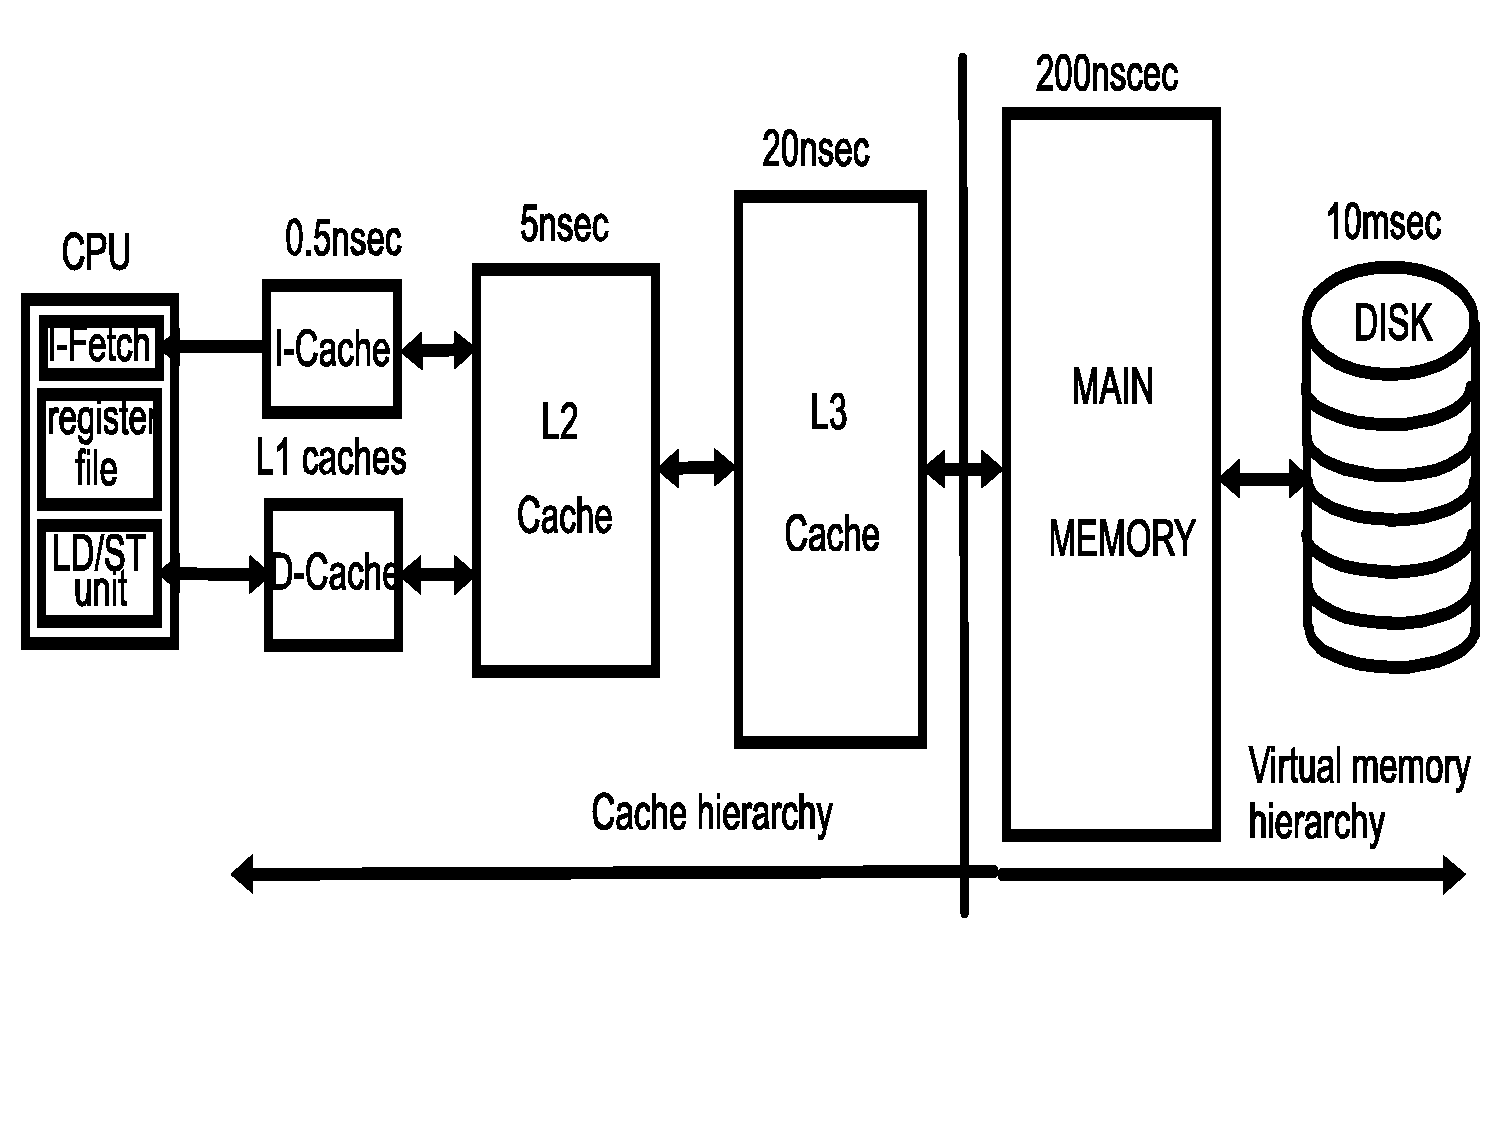
\includegraphics[width=44ex]{Figures/FigsMemH/MemHierarchy}
\column{0.30\textwidth}
\emph{Memory goes at electronic speed}, \emp{Disk at mechanical speed.}
\end{columns}
\vspace{-5ex}

\emph{Locality Principle:}\pause
\begin{itemize}
    \begin{scriptsize}
    \item small set of addresses accessed at a time, 
            named \emph{working set}, $\Rightarrow$ low miss rate,
    \item when program transitions $\Rightarrow$ abrupt change of working sets 
            $\Rightarrow$ high miss rate,
    \item \emph{Temporal Locality:} a referenced item is likely to be accessed again soon,
    \item \emph{Spatial Locality:} items close-by a referenced item likely to be accessed soon,
    \item \emph{Spatial $\Rightarrow$ Temporal} at block/page level.
    \end{scriptsize} 
\end{itemize}
\end{frame}

\begin{frame}[fragile,t]
\frametitle{Typical Memory Hierarchy}

\begin{columns}
\column{0.6\textwidth}
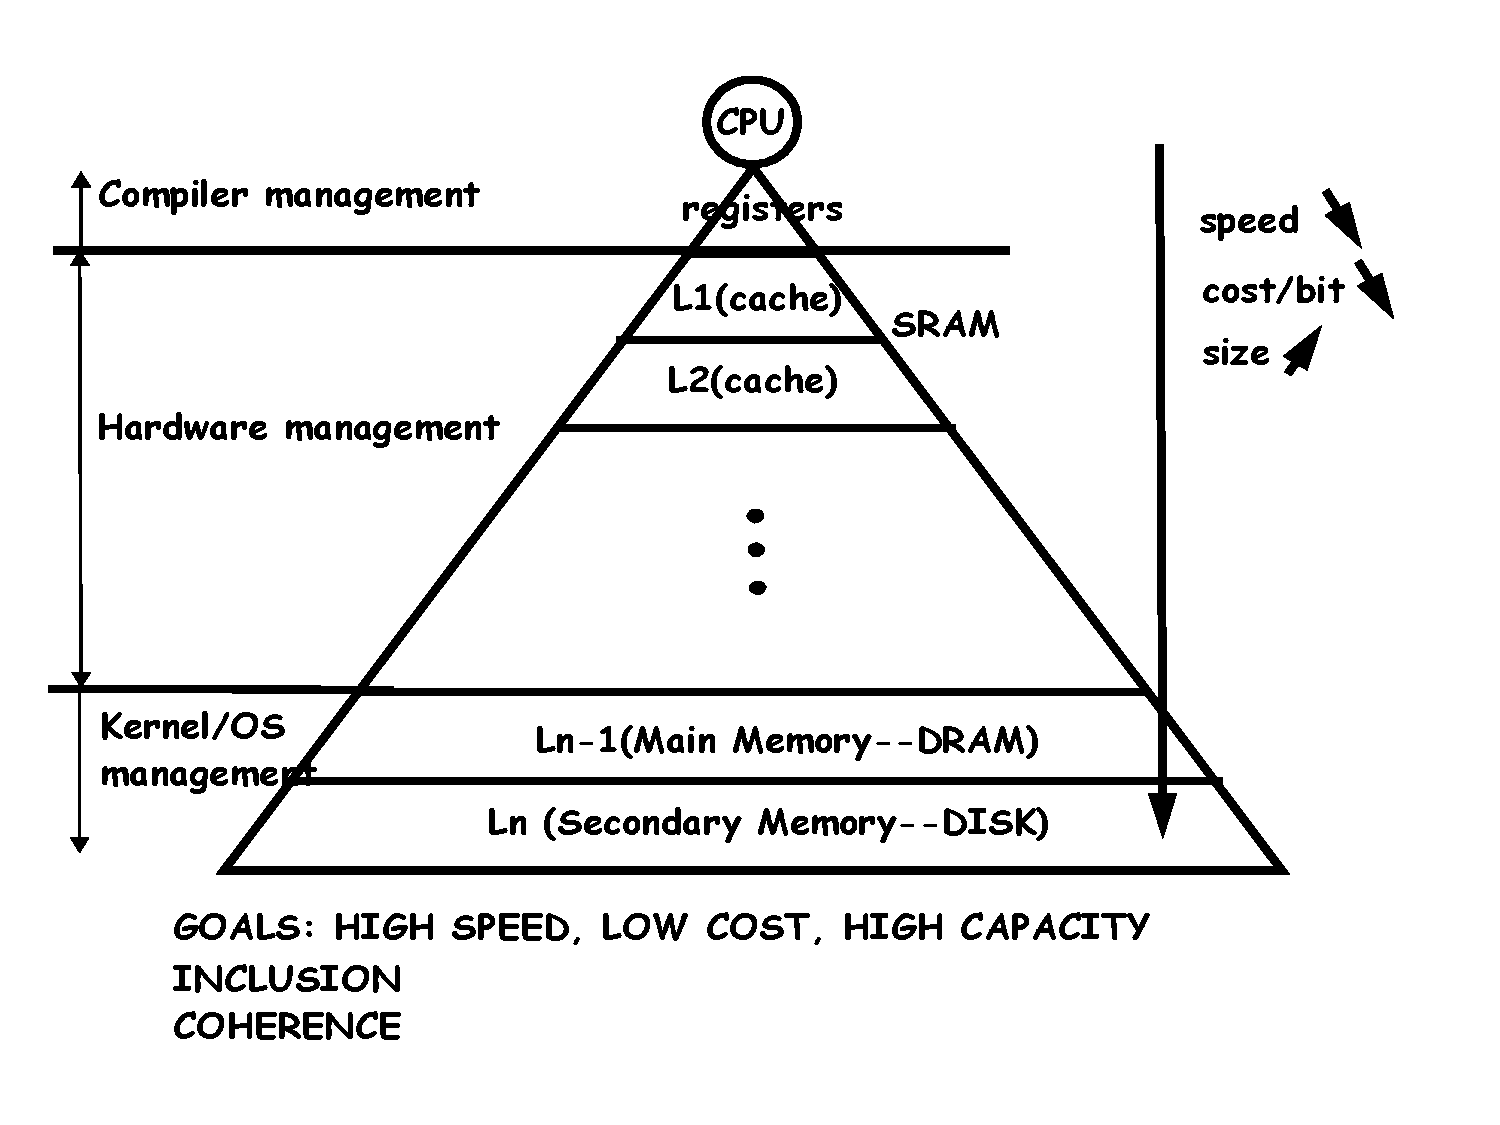
\includegraphics[width=44ex]{Figures/FigsMemH/Pyramid}
\column{0.37\textwidth}
\pause
\begin{scriptsize}
\begin{itemize}
\item \emph{Illusion of a monolithic memory of lowest cost, largest capacity \&
            fastest average access time.}\\
\smallskip
\item \emp{Larger caches are slower} because speed dominated by wire delays
    (do not scale with technology).
\end{itemize}
\end  {scriptsize}
\end{columns}

\begin{itemize}
\begin{scriptsize}
    \item \emp{Coherence} for single cores: instrs executed out of order \& speculatively, but
            the result is as if instrs executed one at a time in program order \& monolithic memory\pause 
            or ``a load must return the value of the previous store to the same address''.
    \item \emp{Inclusion:} Cache level {\tt j} includes {\tt i} ({\tt j > i}) $\Rightarrow$ locations at level {\tt i} are also cached \& has same or more restrictive rights than level {\tt j}. (Helps coherence.)\\
%Level-{\tt i} cache needs not be looked up if block not present at level {\tt j}.
\end{scriptsize}
\end{itemize}
\end{frame}

%%%%%%%%%%%%%%%%%%%%%%%%%%%%%%%%%%%%%%%%%%%%%%%%%%%
%%%%%%%%%%%%%%%%%%%%%%%%%%%%%%%%%%%%%%%%%%%%%%%%%%%
%%%%%%%%%%%%%%%%%%%%%%%%%%%%%%%%%%%%%%%%%%%%%%%%%%%
\section{Cache Design}

\begin{frame}[fragile]
	\tableofcontents[currentsection]
\end{frame}

\begin{frame}[fragile,t]
\frametitle{Cache Performance}

\begin{itemize}
\begin{scriptsize}
\item \emp{Average Memory Access Time} ({\tt AMAT}):\\
        {\tt AMAT $=$ hit time + miss rate $\times$ miss penalty}\bigskip

\item \emp{Miss Rate $\equiv$ 1.0 - Hit Rate} $\equiv$ \% of accesses not satisfied at highest level:\\
        {\tt Miss Rate $\equiv$ (\# misses in L1) / (\# processor references)}  \bigskip

\item Misses Per Instruction ({\tt MPI}):\\
        {\tt MPI $=$ (\# misses in L1) / (\# instructions)}\\
        \emph{Easier to use than Miss Rate:} {\tt CPI $=$ CPI$_0$ + MPI$\times$MissPenalty}\\\bigskip

\item \emp{Miss Penalty}: average delay per miss caused in the processor:\\
        If processor blocks on misses $\Rightarrow$ miss latency (time to bring a block from mem)\\
        In an OoO processor cannot be measured directly $\neq$ miss latency\\\bigskip
\item \emp{Miss Rate and Penalty} can be defined at every cache level. Normalized to:\\
            \# of processor references or\\
            \# of accesses from the lower level.
\end  {scriptsize}
\end{itemize}

\end{frame}

\subsection{Cache Mappings}

\begin{frame}[fragile,t]
\frametitle{Cache Mapping}
 
\begin{itemize}
    \item Cache behavior mostly dictated by: cache size and
    \item {\bf The mapping} of \emp{memory blocks} to \emph{cache lines}.\\
            (Each cache line hosts multiple mem blocks at different times.)
    \item {\em direct or set-associative or fully-associative mapping}.\smallskip
\end{itemize}
\begin{columns}
\column{0.45\textwidth}
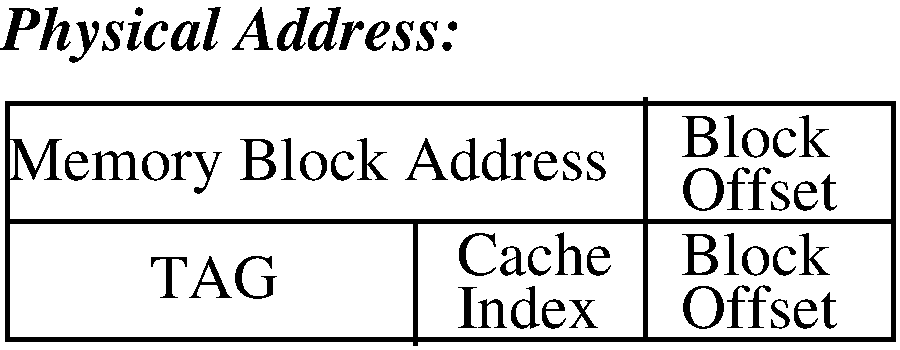
\includegraphics[width=25ex]{Figures/FigsMemH/CacheMapping}
\column{0.50\textwidth}
\begin{scriptsize}
Cache Acess Has Two Phases:
\begin{itemize}
    \item[cache index] use index bits to fetch {\tt tags} and data from the set,
    \item[tag check] check {\tt tag} to detect hit/miss (and status bits).
\end{itemize} 
\end  {scriptsize}
\end{columns}

\bigskip
Cache:
\begin{itemize}
    \item \emph{Data Memory}, i.e., the cached copy of the memory block + 
    \item \emp{Directory Memory}, one entry per cache line containing\\ 
            {\tt TAG} ({\tt ID}) \& status bits: valid, dirty, reference, cache coherence.\\\smallskip
\end  {itemize}

\end{frame}

\begin{frame}[fragile,t]
\frametitle{Direct-Mapped Cache}
 
{\em Cache Slicing:} a memory block mapped always in (the same) cache line, of index:
{\tt (Block Address) mod (\# of cache lines)}.\bigskip
\vspace{-3ex}
\begin{columns}
\column{0.65\textwidth}
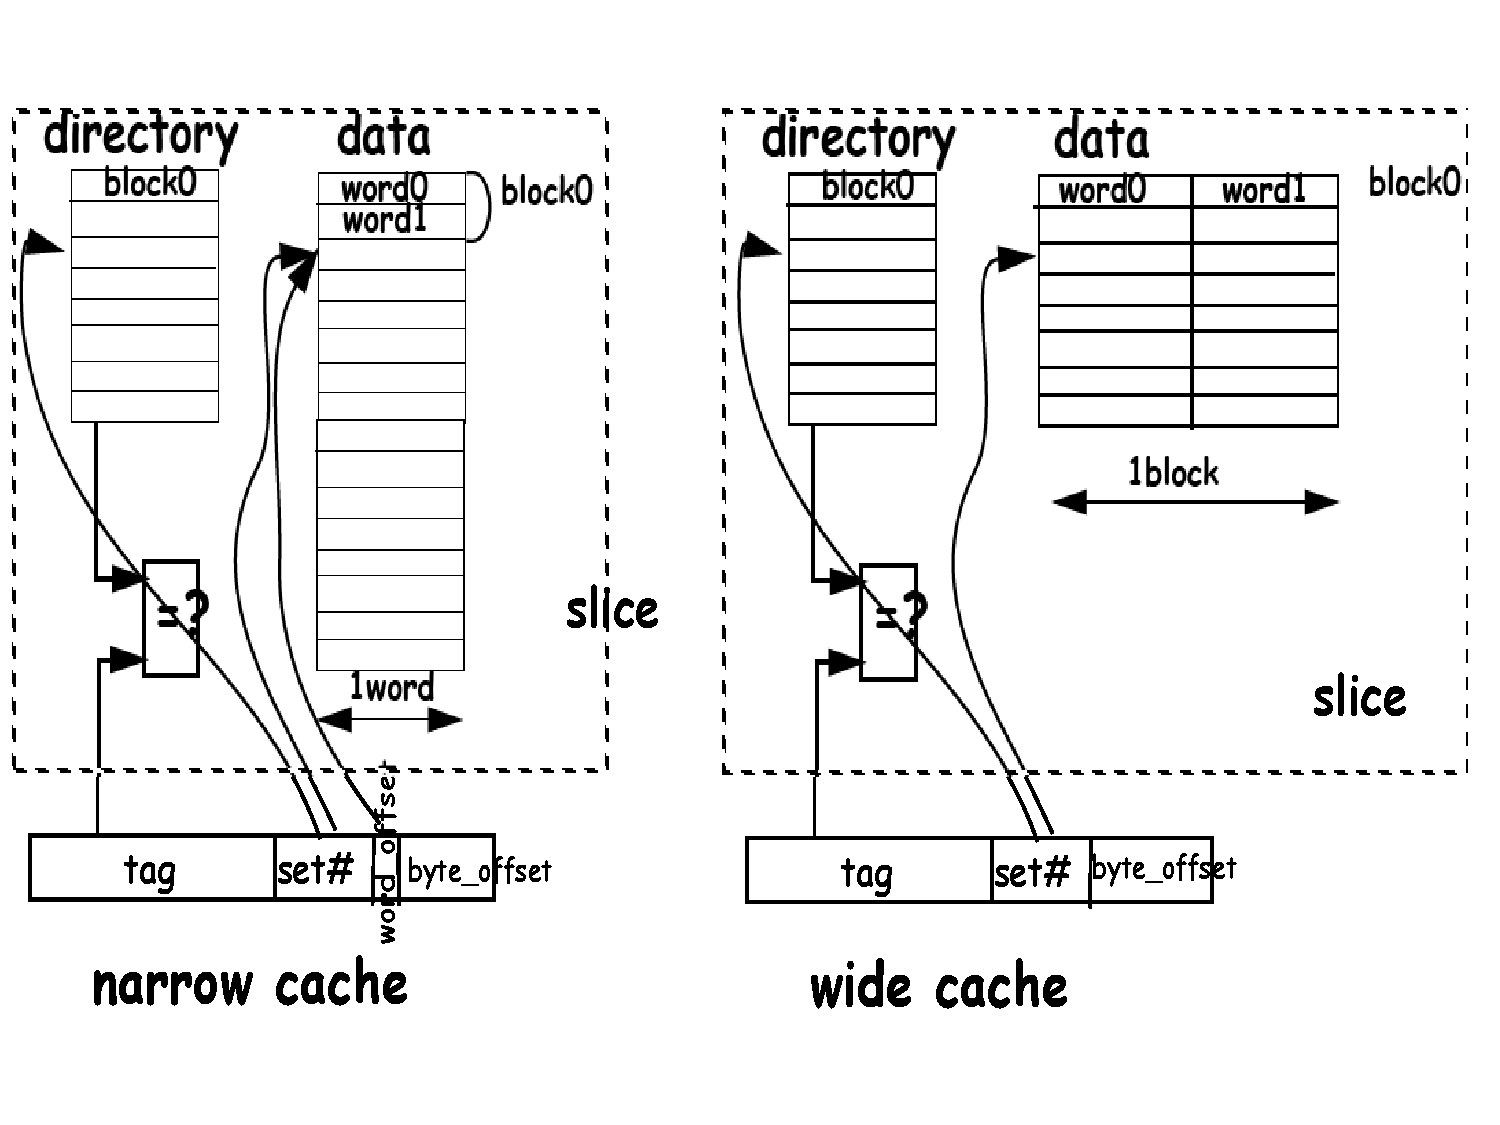
\includegraphics[width=44ex]{Figures/FigsMemH/CacheWide}
\column{0.32\textwidth}
\begin{scriptsize}
{\bf Two Phases:}\\
\emp{Index} + \emph{Tag Check}
\bigskip

\emp{Data-Entry Size:}\\ 
\begin{itemize}
    \item narrow (1 word) $\rightarrow$\\wide (1 cache line)
    \item[wide:] on a miss, the data is reloaded in one cycle of data mem.
    \item[narrow:] less complexity.
\end{itemize} 
\end  {scriptsize}
\end{columns}

\begin{itemize}
    \item[\emph{+}]  fast access time on a hit
    \item[\alert{-}] several blocks competing on the same line $\Rightarrow$ high miss rate 
\end  {itemize}

\end{frame}


\begin{frame}[fragile,t]
\frametitle{Set-Associative Cache}
 
Cache is partitioned into a set of lines:
\begin{itemize}
    \item \emp{access to each set is directly mapped}, but
    \item \emph{a block mapped to a set can reside anywhere in the set}!
\end  {itemize} 

\begin{itemize}
    \item[read] requires one cycle: all 3 directory and data entries fetched in {\tt ||},\\
                then the tag is compared in {\tt ||} with the tag bits of each slice\\
                a hit selects the corresponding word, all misses $\Rightarrow$ cache miss! 
    \item[write] requires at least two mem cycles (can be pipelined): one to check the hit or miss, 
                and then one to write into data memory. 
                 
\end  {itemize}


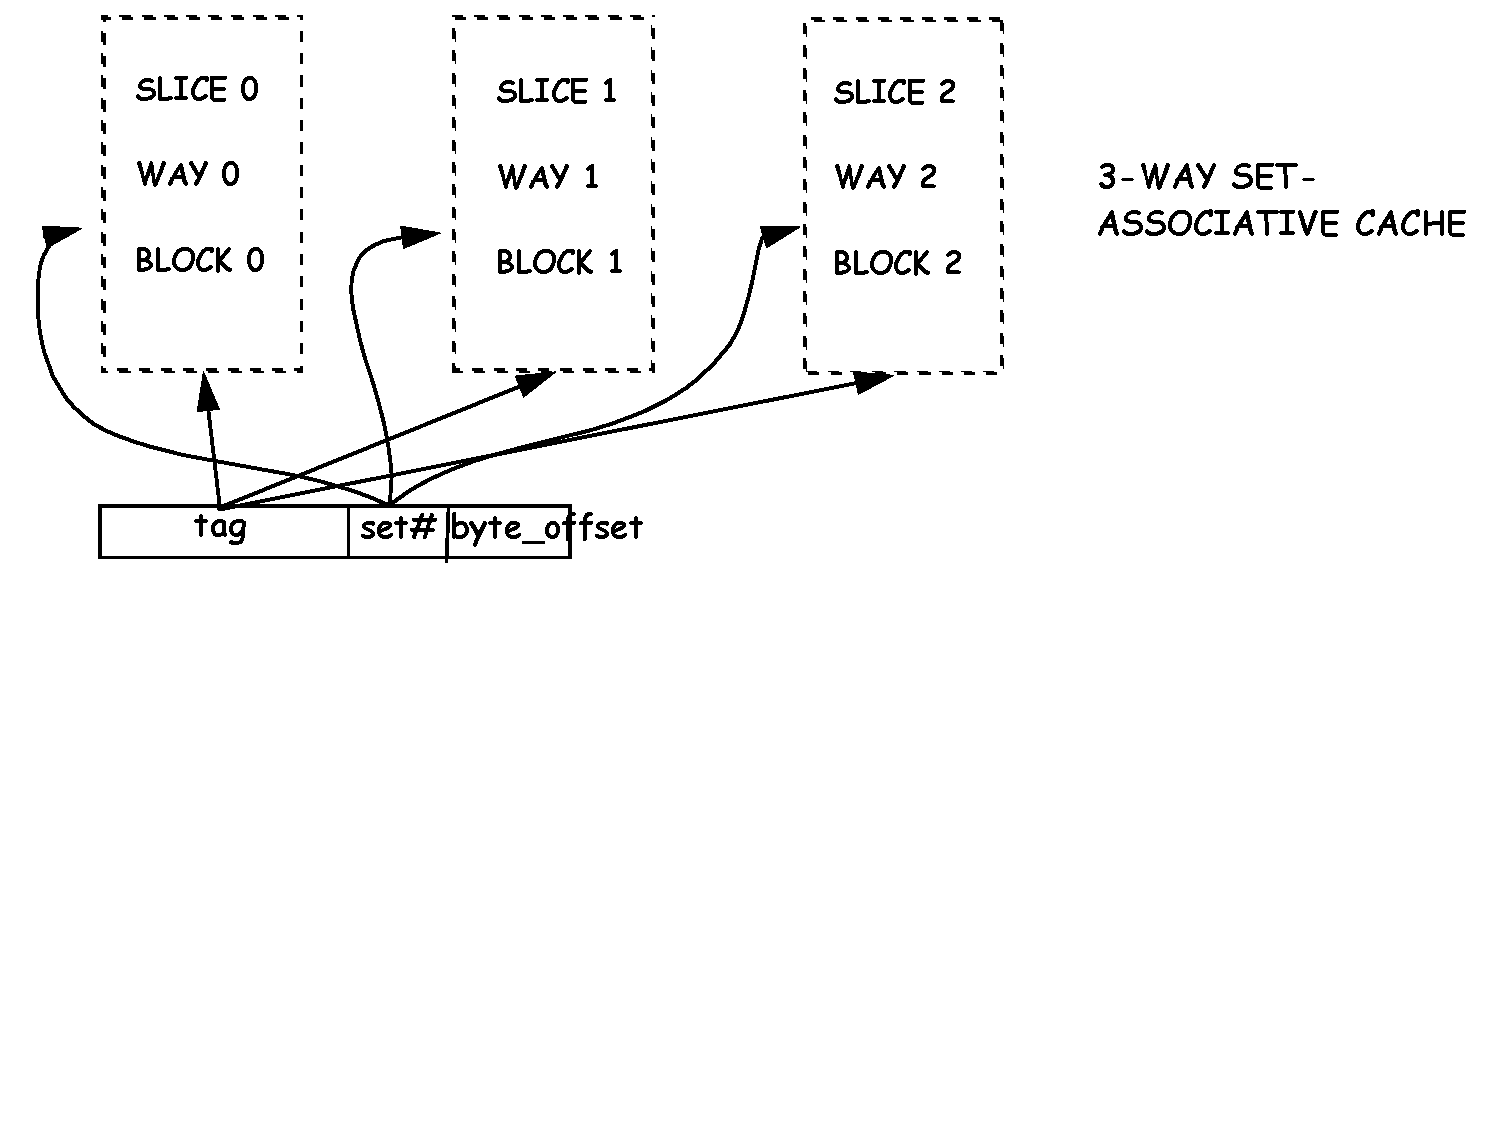
\includegraphics[width=55ex]{Figures/FigsMemH/SetAssoc}

\end{frame}


\begin{frame}[fragile,t]
\frametitle{Full-Associative Cache}
 
Very different structure than an all-way set-associative cache:\\
to find the block all directories must be checked in {\tt ||}!

\begin{columns}
\column{0.4\textwidth}
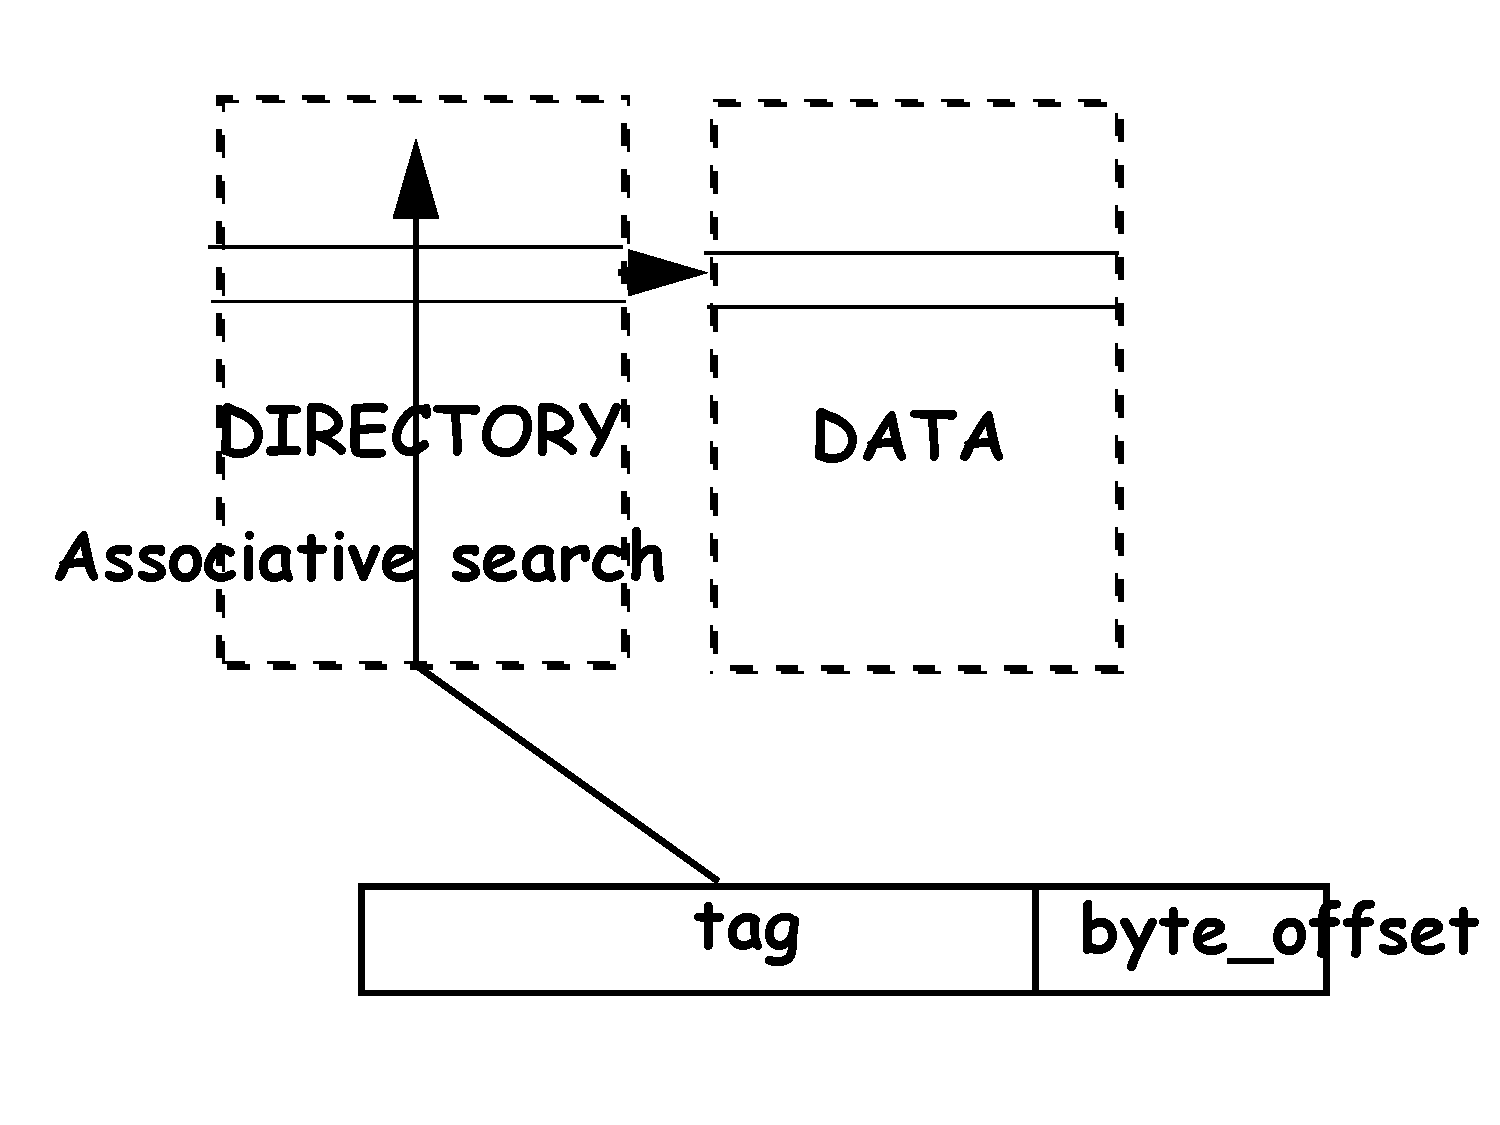
\includegraphics[width=33ex]{Figures/FigsMemH/FullAssoc}\pause
\column{0.55\textwidth}
%\begin{scriptsize}
Two Steps:
\begin{itemize}
    \item \emp{{\tt||} tag check} $\Rightarrow$ tag bus lines throughout the directory; 
            comparator associated with each dir entry, then
    \item  \emph{on match} the row line is activated and data returned.
    \item \emp{load \& store requires 2 cycles.}
\end  {itemize} 
%\end{scriptsize}
\end{columns}
\medskip

Content-Addressable Memory (CAM) \emp{slower \& less dense} than RAM.\\
(signal propag, comparison, etc.)\bigskip

Small Caches: fully associative because potential for conflict in hot sets
    is damaging to performance. 

\end{frame}

\subsection{Replacement \& Write (Back/Through) Policies}
\begin{frame}[fragile,t]
\frametitle{Replacement Policies (Selects a Victim Block)}

Random, Least Recently Used (LRU), FIFO, Pseudo-LRU:\\
    {\tt~~~~}maintain replacement bits.

\vspace{-2ex}
\begin{columns}
\column{0.7\textwidth}
\hspace{-5ex}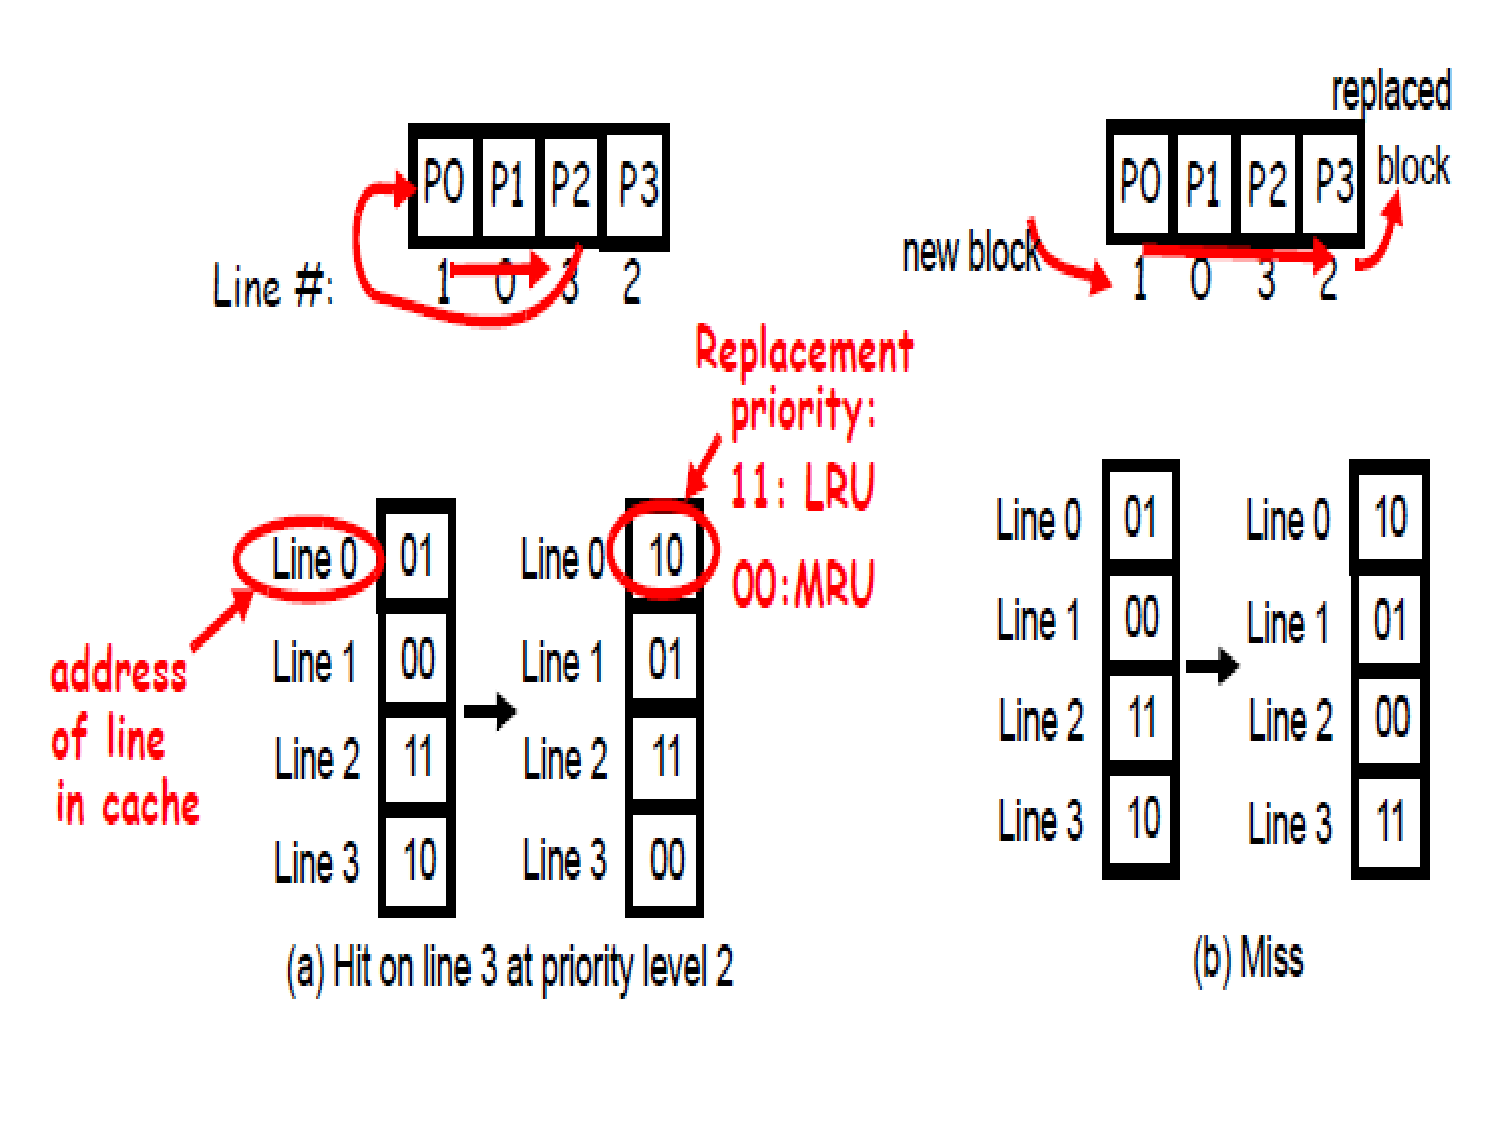
\includegraphics[width=50ex]{Figures/FigsMemH/LRU}\pause
\column{0.2\textwidth}
$\Leftarrow$ LRU Example:
\end{columns}
\vspace{-2ex}
\emp{Direct Mapper $\Rightarrow$ No Need.}\\
\emp{Set/Fully Associative $\Rightarrow$ Per-Set/Cache Replacement.}

\end{frame}


\begin{frame}[fragile,t]
\frametitle{Write Policies}

%\emp{Write Through} to next level on all writes
\begin{columns}
\column{0.51\textwidth}
\hspace{-4ex}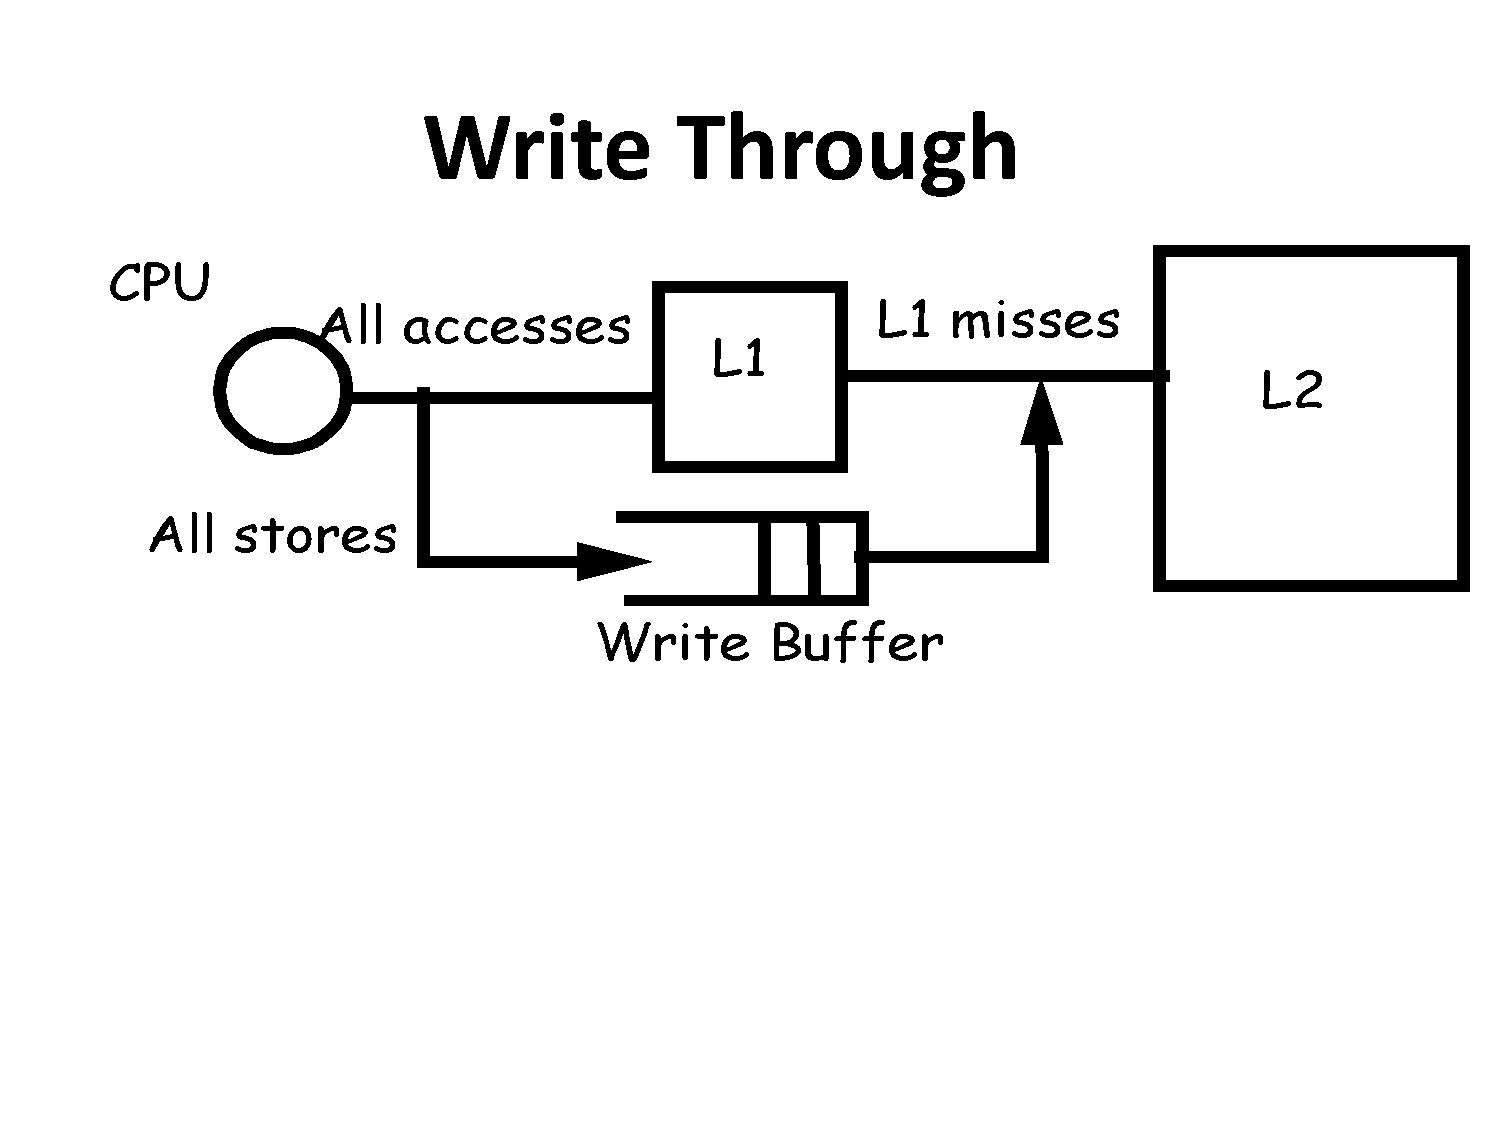
\includegraphics[width=40ex]{Figures/FigsMemH/WriteThrough}\pause
\column{0.46\textwidth}
\vspace{-8ex}
\begin{itemize}
\begin{scriptsize}
    \item {\bf write to next level on all writes}
    \item use a write buffer to avoid stalls;\\
            loads must check the buffer first!
    \item Used for small 1st-level caches: 
    \item \emph{simple, no inconsistency on levels}
    \item but \emp{large store traffic}
\end  {scriptsize}
\end  {itemize}
\end{columns}

\vspace{-8ex}
\begin{columns}
\column{0.44\textwidth}
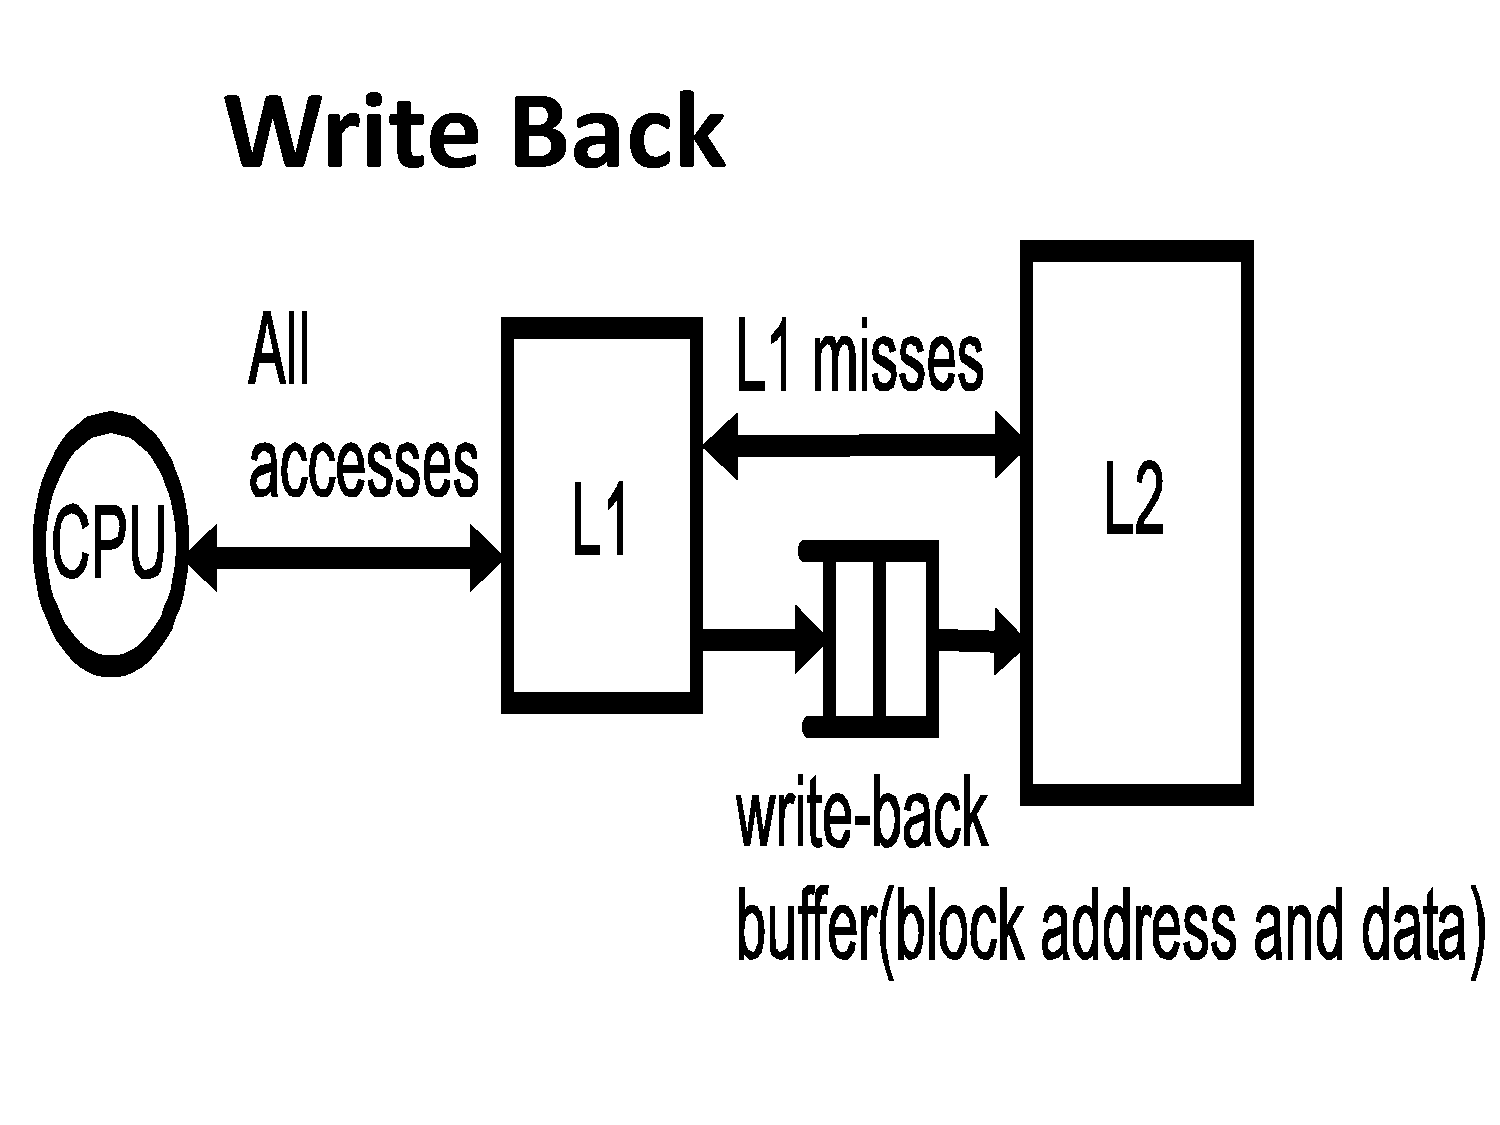
\includegraphics[width=35ex]{Figures/FigsMemH/WriteBack}\pause
\column{0.53\textwidth}
\vspace{-3ex}
\begin{itemize}
\begin{scriptsize}
    \item {\bf write to next level on replacement}
    \item uses a dirty bit ({\tt db}) \& write-back buffer\\
            block is loaded/modified $\Rightarrow$ {\tt db} reset/set\\
            block is evicted $\Rightarrow$ if {\tt db} set then written.
    \item \emph{write happens only on a miss}\smallskip

    \item IN BOTH CASES: a load checks the buffer first (consistency)!
    \item Write Miss: always allocate on write back; design choice in write through!
%    \item On a write miss: (i) Write-Back always allocates; (ii) design choice in write through. 
\end  {scriptsize}
\end  {itemize}\bigskip
\end{columns}
\end{frame}


\subsection{The Four Types of Cache Misses}
\begin{frame}[fragile,t]
\frametitle{Classification of Cache Misses}

The Four C's:
\begin{itemize}
\begin{scriptsize}
\item[Cold] (Compulsory) misses: first reference of a block,\smallskip

\item[Capacity] misses: insufficient space for data/code,\smallskip

\item[Conflict] misses: two memory blocks map to the same cache line,\smallskip

\item[Coherence] misses, e.g., another thread has modified the needed value.\bigskip
\end  {scriptsize}
\end{itemize}

How to measure them:\pause
\begin{itemize}
\begin{scriptsize}
\item[Cold:] simulate infinite cache size,\smallskip

\item[Capacity:] simulate fully-assoc cache and subtract cold misses\smallskip

\item[Conflict:] simulate cache and subtract cold and capacity misses.\bigskip
\end  {scriptsize}
\end{itemize}

\end{frame}


\begin{frame}[fragile,t]
\frametitle{Multi-Level Cache Hierarchies}

\begin{columns}
\column{0.65\textwidth}
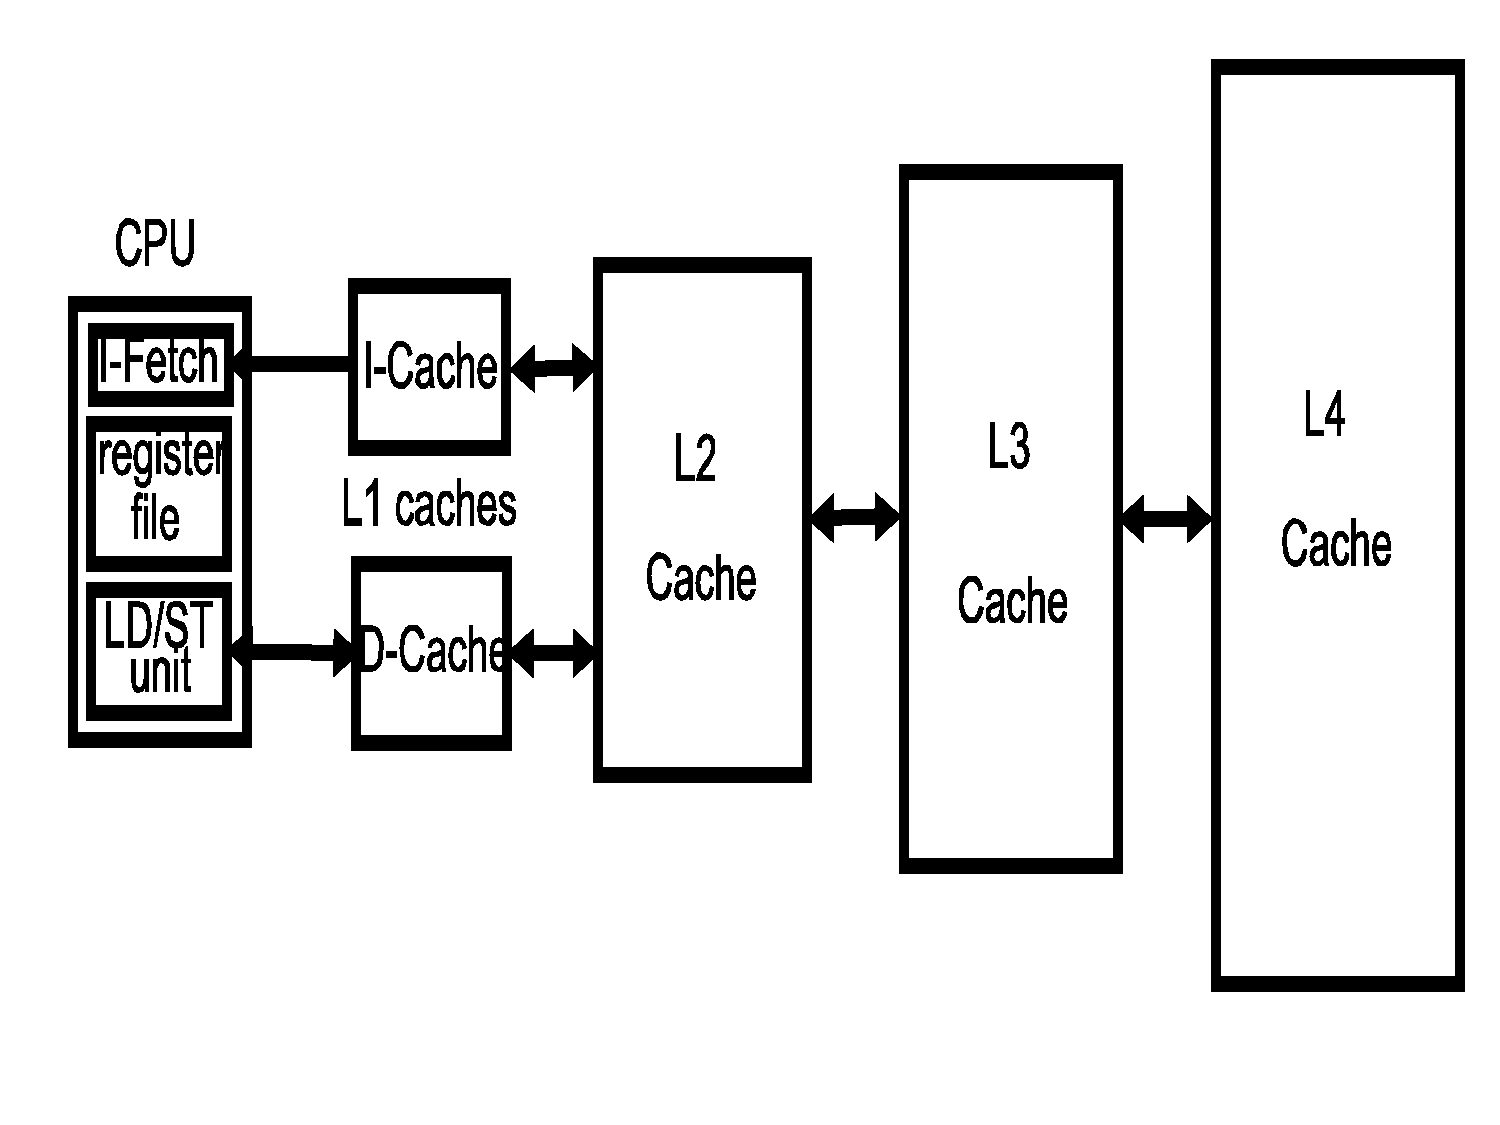
\includegraphics[width=35ex]{Figures/FigsMemH/MultiLevCache}
\column{0.3\textwidth}
1st and 2nd levels on chip; 3rd and 4th mostly off chip\smallskip
\end{columns}

We will assume \emph{Cache Inclusion}. A block
\begin{scriptsize}
\begin{itemize}
    \item misses in $L_i$ $\Rightarrow$ must be brought in all $L_j, j>i$.
    \item is replaced in $L_j$ $\Rightarrow$ must be removed in all $L_i, j>i$.
    \item \emp{replication} but \emph{good for coherence}.
\end  {itemize}
\end  {scriptsize}\bigskip

\emp{Cache Exclusion.} A block:
\begin{scriptsize}
\begin{itemize}
    \item is in $L_i$ $\Rightarrow$ then it is not in any other level.
    \item misses in $L_i$ $\Rightarrow$ all copies are removed from all levels $> i$.
    \item is replaced in $L_j$ $\Rightarrow$ allocated in $j+1$.
    \item \emph{size is the sum of all caches}, but \emp{horrible for coherence}.
\end  {itemize}
\end  {scriptsize}\bigskip

\end{frame}


\begin{frame}[fragile,t]
\frametitle{Cache Parameters}

Large Caches: slower (wire delays), more complex, less capacity misses.\bigskip

Larger Block Size: 
\begin{itemize}
    \item exploits spatial locality, but
    \item if too big $\Rightarrow$ capacity misses $\uparrow$
    \item big blocks increase miss penalty.\bigskip
\end  {itemize}

Higher Set Associativity (SA): 
\begin{itemize}
    \item addresses conflict misses
    \item 8-16 ways SA as good as fully associative
    \item A 2-way SA cache of size $N$ has similar 
            miss rate with a direct mapped of size $2\times N$.
    \item Higher hit time.
\end  {itemize}
\end{frame}

\section{Improving Performance: Lockup-Free Cache and Prefetching}

\begin{frame}[fragile]
	\tableofcontents[currentsection]
\end{frame}


\begin{frame}[fragile,t]
\frametitle{Lockup-Free Caches}

\begin{columns}
\column{0.5\textwidth}
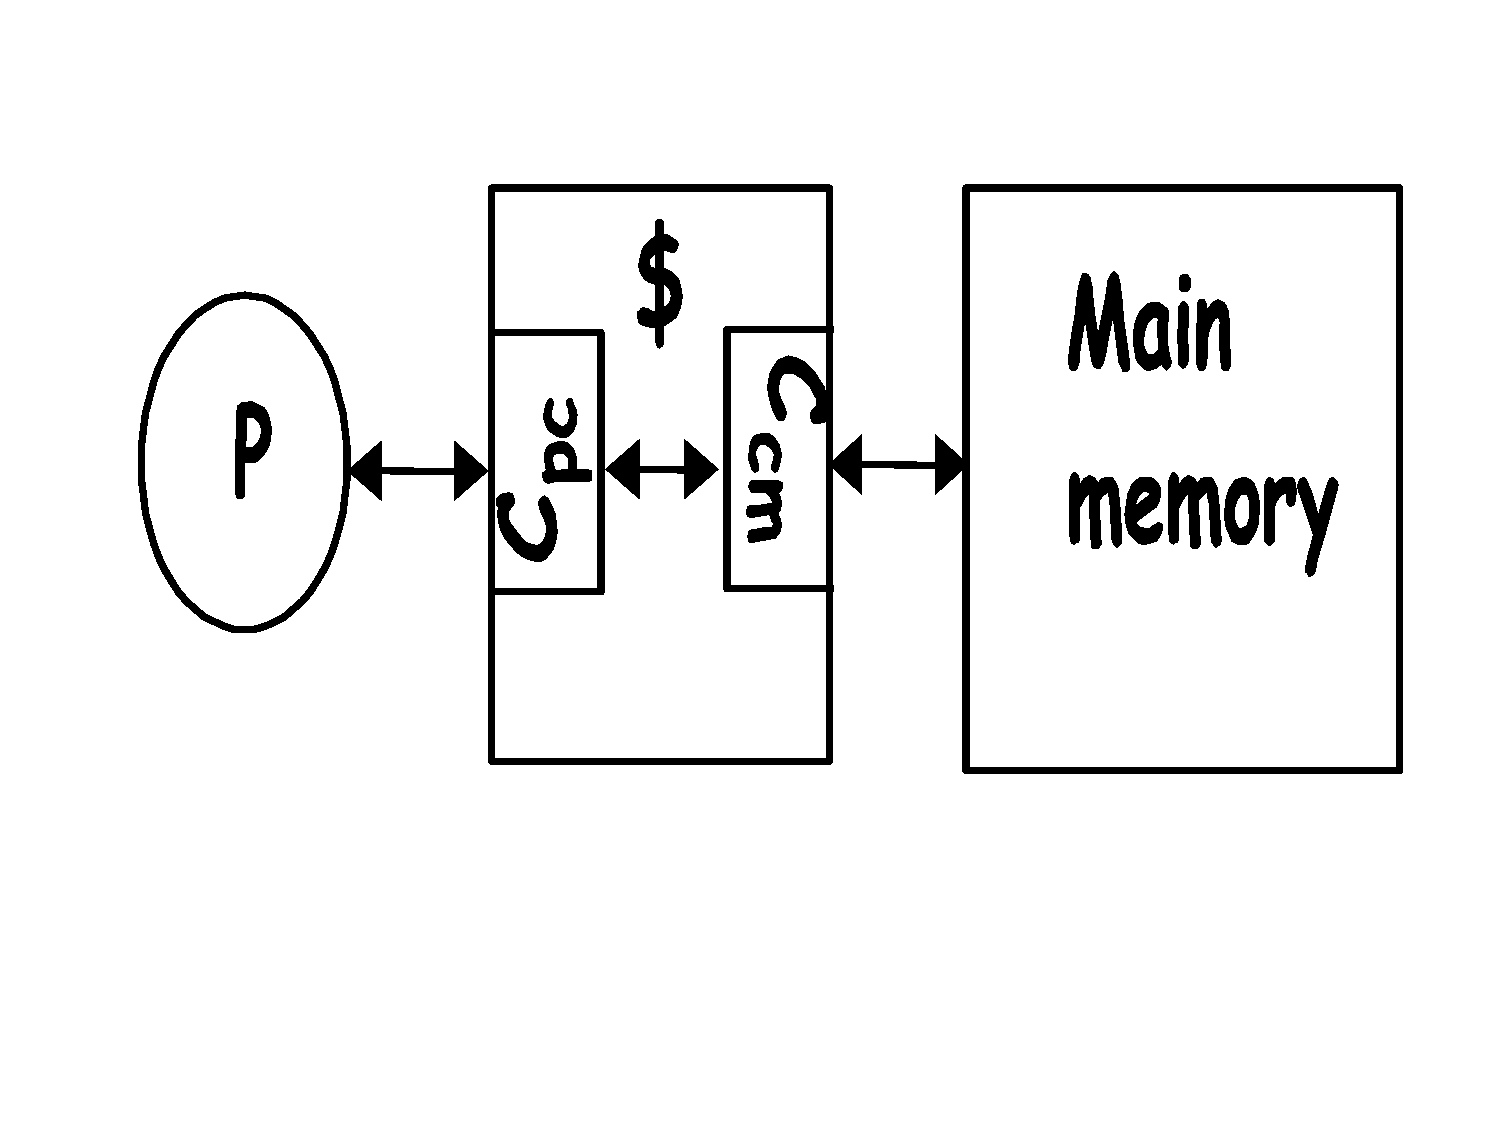
\includegraphics[width=35ex]{Figures/FigsMemH/CpcCcm}
\column{0.47\textwidth}
Cache is a Two-Ported Device:\\
Memory \& Processor.\smallskip

$C_{pc}:$ cache to processor interf\smallskip

$C_{cm}:$ cache to memory interface
\end{columns}
\vspace{-3ex}

\begin{itemize}
\begin{scriptsize}
    \item Needed to support Prefetching \& Dynamically-Scheduled OoO Single Proces 
            \& Core MultiThreading \& Multi Cores
    \item A Lockup-Free Cache does not block on a miss, but keeps accepting proc requests,
    \item hence, it allows concurrent processing of multiple hits/misses.
    \item Cache has to bookkeep all pending misses:
        \begin{itemize}
        \begin{scriptsize}
            \item Miss Status Handling Register ({\tt MSHR}) contains 
                    address of the pending miss $+$ destination block in cache $+$ 
                    destination register.
            \item {\tt MSHR} used to complete a miss and 
                    to avoid sending multiple miss requests per block.
                    \# of {\tt MSHR}s limits the \# of pending misses (at a time).
        \end{scriptsize} 
        \end  {itemize}
    \item Data dependencies eventually block the processor.
\end {scriptsize}
\end  {itemize}
\end{frame}

\begin{frame}[fragile,t]
\frametitle{Lockup-Free Caches (Continuation)}


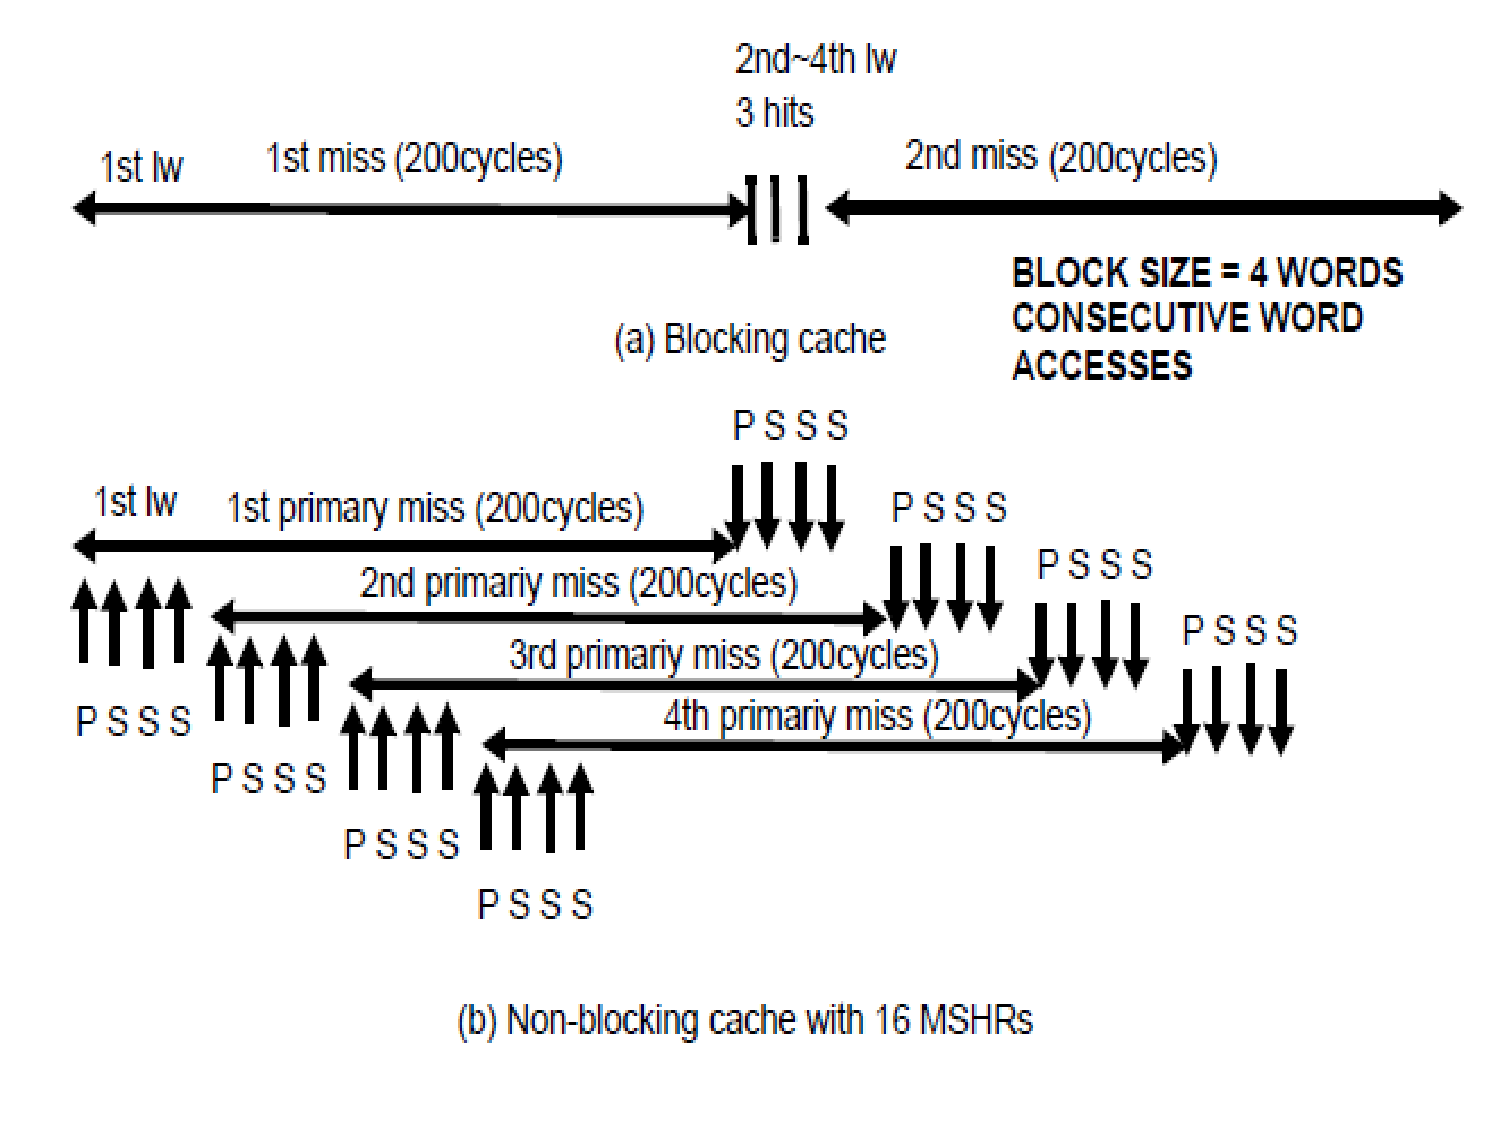
\includegraphics[width=44ex]{Figures/FigsMemH/PrimSecMiss}

\begin{itemize}
    \item Primary Miss (P) is the first miss to a block
    \item Secondary Miss (S) next accesses to same block {\scriptsize (due to pending P)} 
        \begin{itemize}
        \begin{scriptsize}
            \item Many more misses than Blocking Cache, which has only Ps.
            \item Needs {\tt MSHR}s for both P and S misses
            \item Misses are overlapped with computation and other misses.
        \end {scriptsize}
        \end  {itemize}
\end  {itemize}
\end{frame}


\begin{frame}[fragile,t]
\frametitle{Hardware Prefetching}

\begin{columns}
\column{0.4\textwidth}
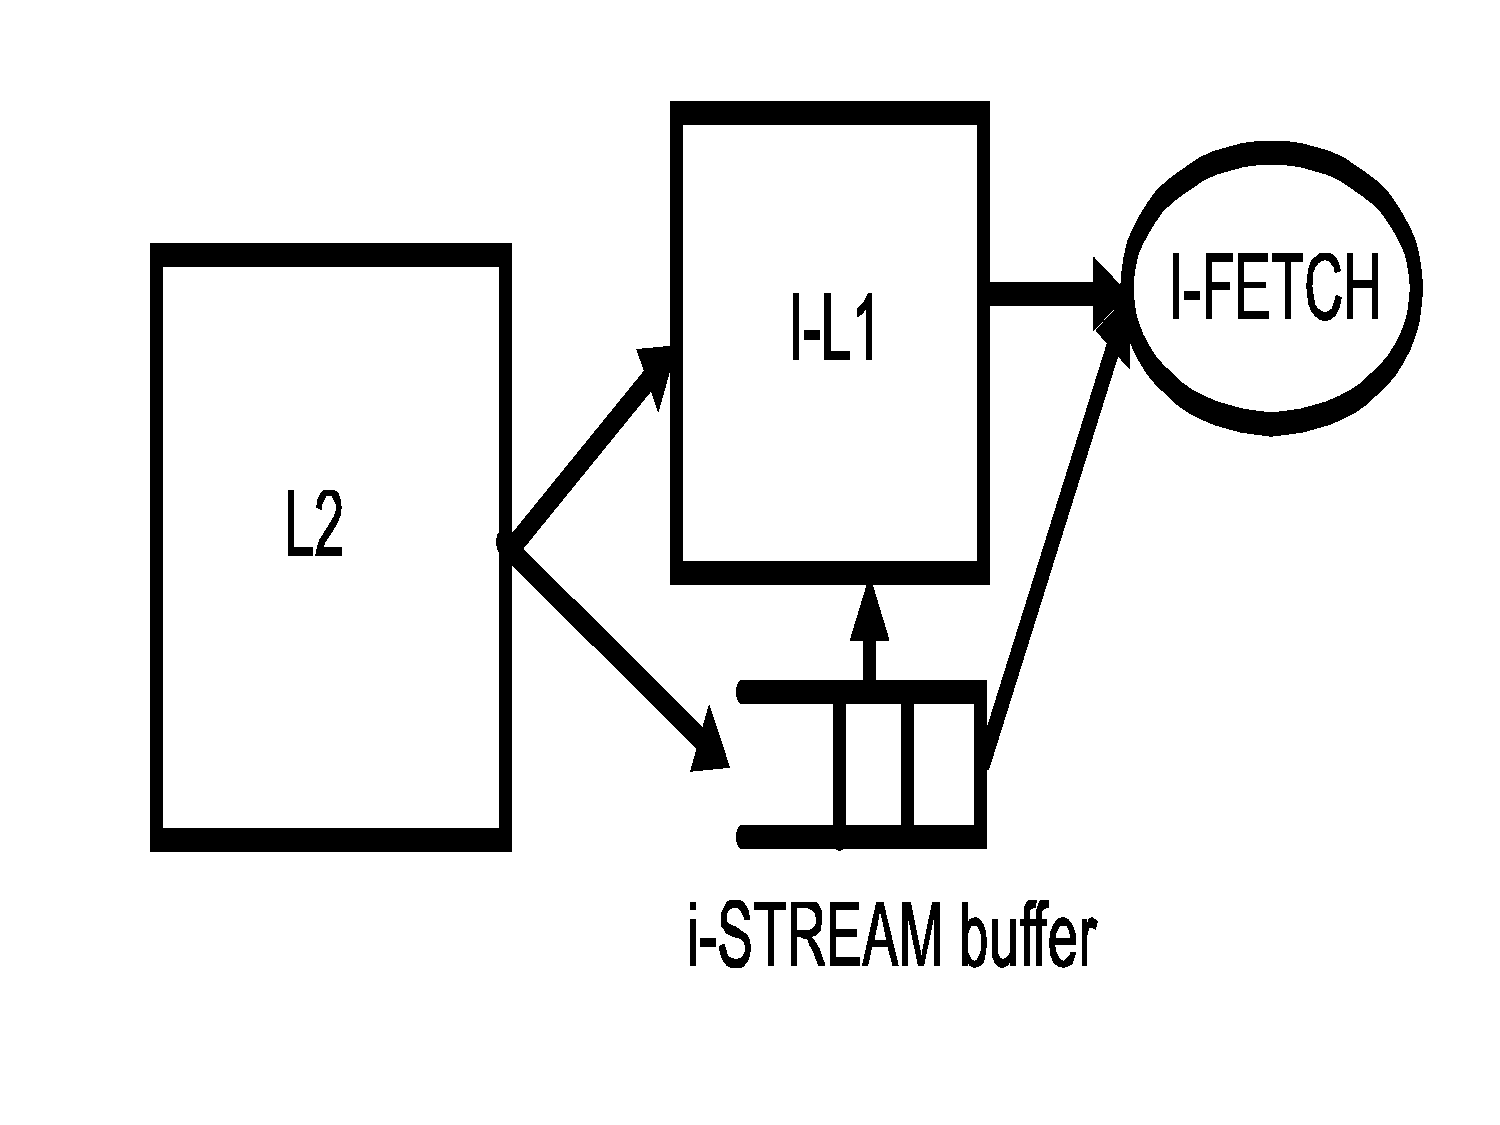
\includegraphics[width=27ex]{Figures/FigsMemH/SeqPrefetching}
\column{0.55\textwidth}
Sequential Prefetching Of Instrs:\smallskip
\begin{scriptsize}
I-Fetch Miss $\Rightarrow$ fetch 2 blocks instead of 1.\\\smallskip
2nd block stored in i-STREAM buffer:\\
(1) If I-STREAM hits $\Rightarrow$ block moved to L1\\
(2) Not accessed $\Rightarrow$ I-STREAM blocks overlaid.\\
(3) Prefetch Buffer avoids cache pollution.\\
(4) Applicable to data but less effective.
\end  {scriptsize}
\end{columns}

\begin{columns}
\column{0.45\textwidth}
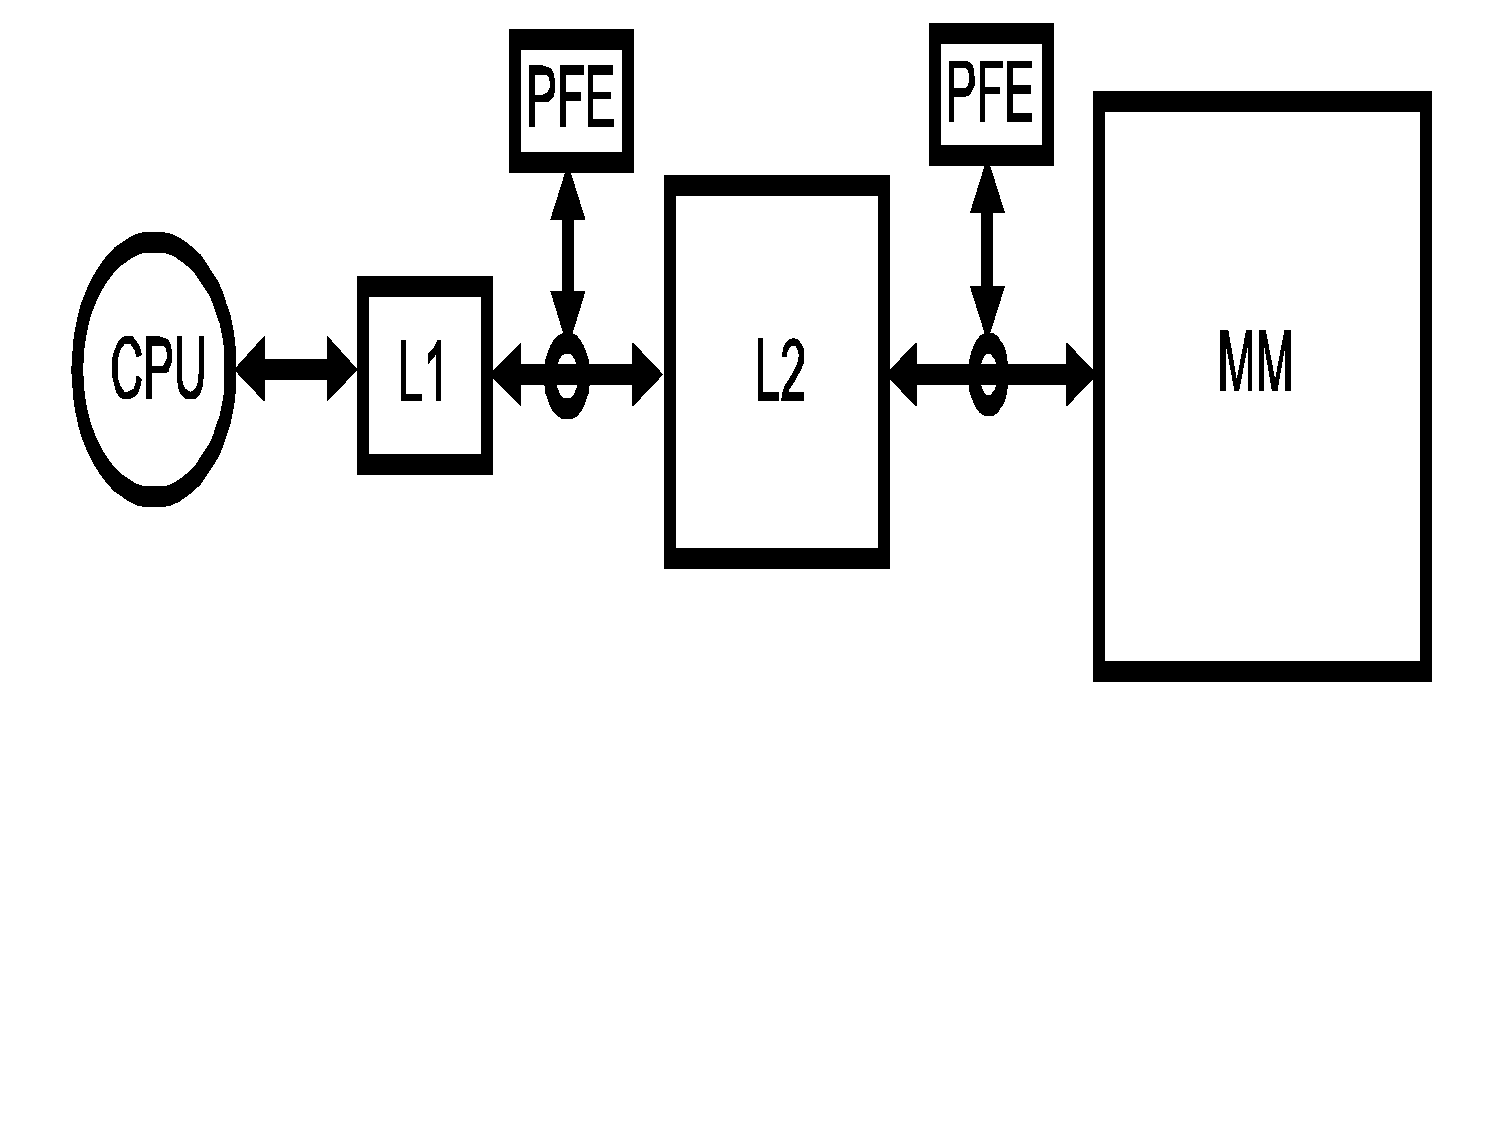
\includegraphics[width=33ex]{Figures/FigsMemH/HwdPrefetching}
\column{0.5\textwidth}
Hardware Prefetch Engines (PFE):\\\smallskip
\begin{scriptsize}
(1) detect strides in stream of missing\\ 
{\tt~~~}addresses by observing the bus then\\
{\tt~~~}start fetching ahead.\\
(2) naturally triggered by speculative exec:\\ 
(3) prefetch is harmless, i.e.,\\
{\tt~~~}exception $\Rightarrow$ prefetch dropped.\\
(4) but might polute caches.
\end  {scriptsize}
\end{columns}

\end{frame}


\begin{frame}[fragile,t]
\frametitle{Software Prefetching}

\begin{itemize}
    \item Prefetch instrs: non-blocking \& non-binding (load in-cache only)
    \item E.g., prefetch instructions may be inserted in the loop's body 
            to prefetch data needed by future iterations:
\end  {itemize}

\begin{block}{HL Code{\tt~~~~~~~~~~~}MIPS Code}\vspace{-2ex}
\begin{columns}
\column{0.18\textwidth}
\begin{colorcode}[fontsize=\scriptsize]
for(i=1000;i>0;i--)
  A[i]=A[i]+s
\end{colorcode} 
\column{0.40\textwidth}
\begin{colorcode}[fontsize=\scriptsize]
Loop: L.D   F2, 0(R1)
      PREF    -24(R1)
      ADD.D F4, F2, F0
      S.D   F4, 0(R1)
      SUBI  R1, R1, #8
      SUBI  R2, R2, #1
      BNEZ  R2, Loop
\end{colorcode} 
\column{0.35\textwidth}
{\tt PREF    -24(R1)}\\
prefetches the elements of {\tt A} 3 iterations ahead.
\end{columns}
\end{block}

\begin{itemize}
    \item Works for both load and stores, but
    \item data must be prefetched at perfect time:\\
            not too early (cache polution), not too late (not in cache),
    \item Instructional overhead \& requires non-blocking cache,
    \item Done for arrays, but also for pointer accesses.
\end  {itemize}
\end{frame}

\begin{frame}[fragile,t]
\frametitle{Faster Hit Times}

Princeton vs Harvard Cache:
\begin{itemize}
    \item Princeton: unified instr/data cache $\Rightarrow$ can use whole cache 
    \item Harvard: split instr/data cache $\Rightarrow$ optimized for access type.
    \item Pipelined Machine: FstLC Harvard \& SndLC Princeton.\bigskip
\end  {itemize}

Pipeline Cache Accesses:
\begin{itemize}
    \item Especially useful for stores:
    \item Pipeline Tag Check and Data Store (2 mem cycles)
    \item Separate Read/Write Ports to cache, optimized for each
    \item Also useful for I-Caches and Load in D-Caches
    \item $\uparrow$ pipeline length, but must split cache accesses into stages!
\end  {itemize}
\end{frame}


\begin{frame}[fragile,t]
\frametitle{What Should First Level Cache (FLC) Be?}
\pause

Keep the cache simple and fast:\smallskip
\begin{itemize}
    \item Favors direct-mapped cache:
        \begin{itemize}
            \item less multiplexing
            \item overlap of tag and use of data.
        \end{itemize}\smallskip
    \item Interestingly, the size of FLC tends to decrease and
            associativity goes up as FLCs try to keep up with CPU.
\end  {itemize}

\begin{scriptsize}
\begin{tabular}{ll}
\hline
Processor    &  L1 Data Cache\\\hline
Alpha 21164  &  8KB, direct mapped\\\hline
Alpha 21364  &  64KB, 2-way\\\hline
MPC 750  &  32KB, 8-way, PLRU\\\hline
PA 8500  &  1MB, 4-way, PLRU\\\hline
Classic Pentium  &  16KB, 4-way, LRU\\\hline
Pentium-II  &  16KB, 4-way, PLRU\\\hline
Pentium-III  &  16KB, 4-way, PLRU\\\hline
Pentium-IV  &  8KB, 4-way, PLRU\\\hline
MIPS R10K/12K  &  32KB, 2-way, LRU\\\hline
UltraSparc-IIi  &  16KB, direct mapped\\\hline
UltraSparc-III  &  64KB, 4-way, random\\\hline
\end{tabular}
\end{scriptsize}
\end{frame}

\section{Architectural Support for Virtual Memory}

\begin{frame}[fragile]
	\tableofcontents[currentsection]
\end{frame}

\begin{frame}[fragile,t]
\frametitle{Why Virtual Memory?}

Allows applications to be bigger than Main Memory.\smallskip

Multiple Process Management:\smallskip
\begin{itemize}
    \item Each processor gets its own chunk of memory:
    \item Protection against each other,
    \item Protection against themselves,
    \item Application and CPU run in virtual space,
    \item Virtual-to-Physical Space Mapping invisible to application,
\end  {itemize}

%\bigskip
%Management between Main Memory (MM) and Disk:\\
%Miss in MM $\Rightarrow$ Page Fault
\end{frame}

\begin{frame}[fragile,t]
\frametitle{Virtual Address Mapping}
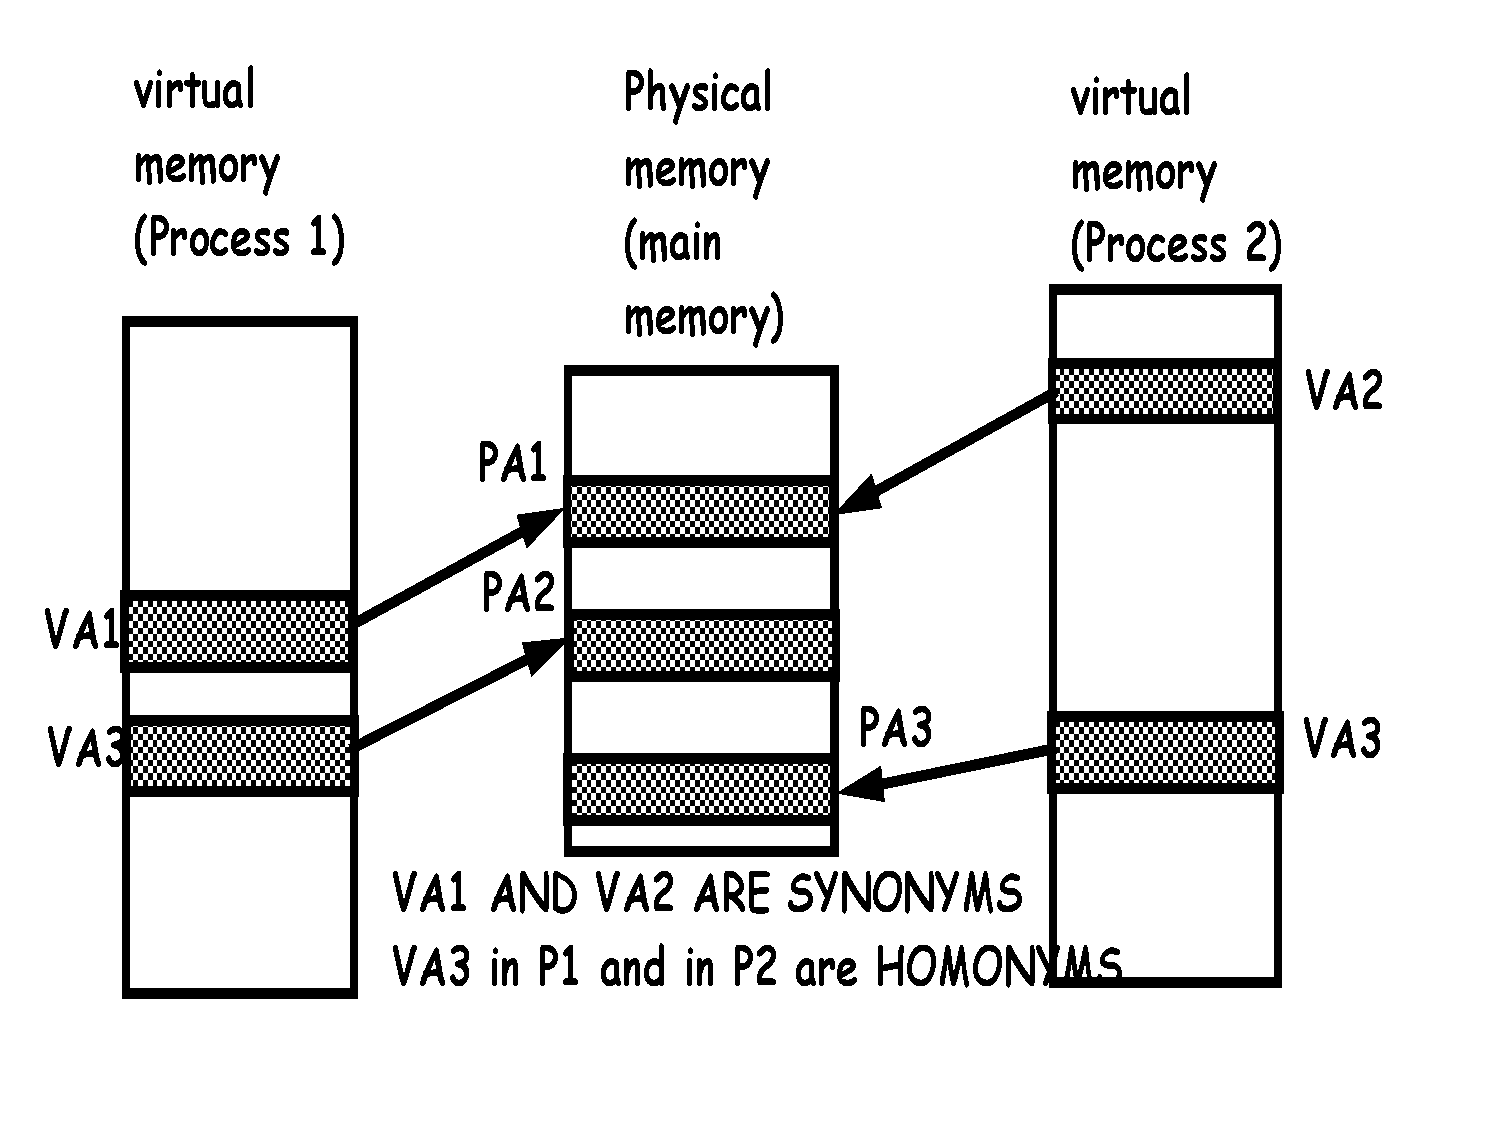
\includegraphics[width=55ex]{Figures/FigsMemH/PageSynHom}

\end{frame}

\begin{frame}[fragile,t]
\frametitle{Paged Virtual Memory}

\begin{itemize}
    \item Virtual address space divided into pages,\bigskip
    \item Physical address space divided into page frames,\bigskip
    \item Page Missing in Main Memory (MM) $\Rightarrow$ Page Fault
        \begin{itemize}
        %\begin{scriptsize}
            \item Pages not in MM are on disk: swapped-in/swapped-out,
            \item or have never been allocated.
            \item New page may be placed anywhere in MM (fully-associative)
        %\end {scriptsize}
        \end  {itemize}\bigskip
    \item Dynamic Address Translation:
        \begin{itemize}
        %\begin{scriptsize}
            \item Effective address is virtual, but
            \item must be translated to physical for every access.
            \item Virtual-to-physical address translation through page table in MM!
        %\end {scriptsize}
        \end  {itemize}
\end  {itemize}

\end{frame}


\begin{frame}[fragile,t]
\frametitle{Page Table}

\begin{columns}
\column{0.55\textwidth}
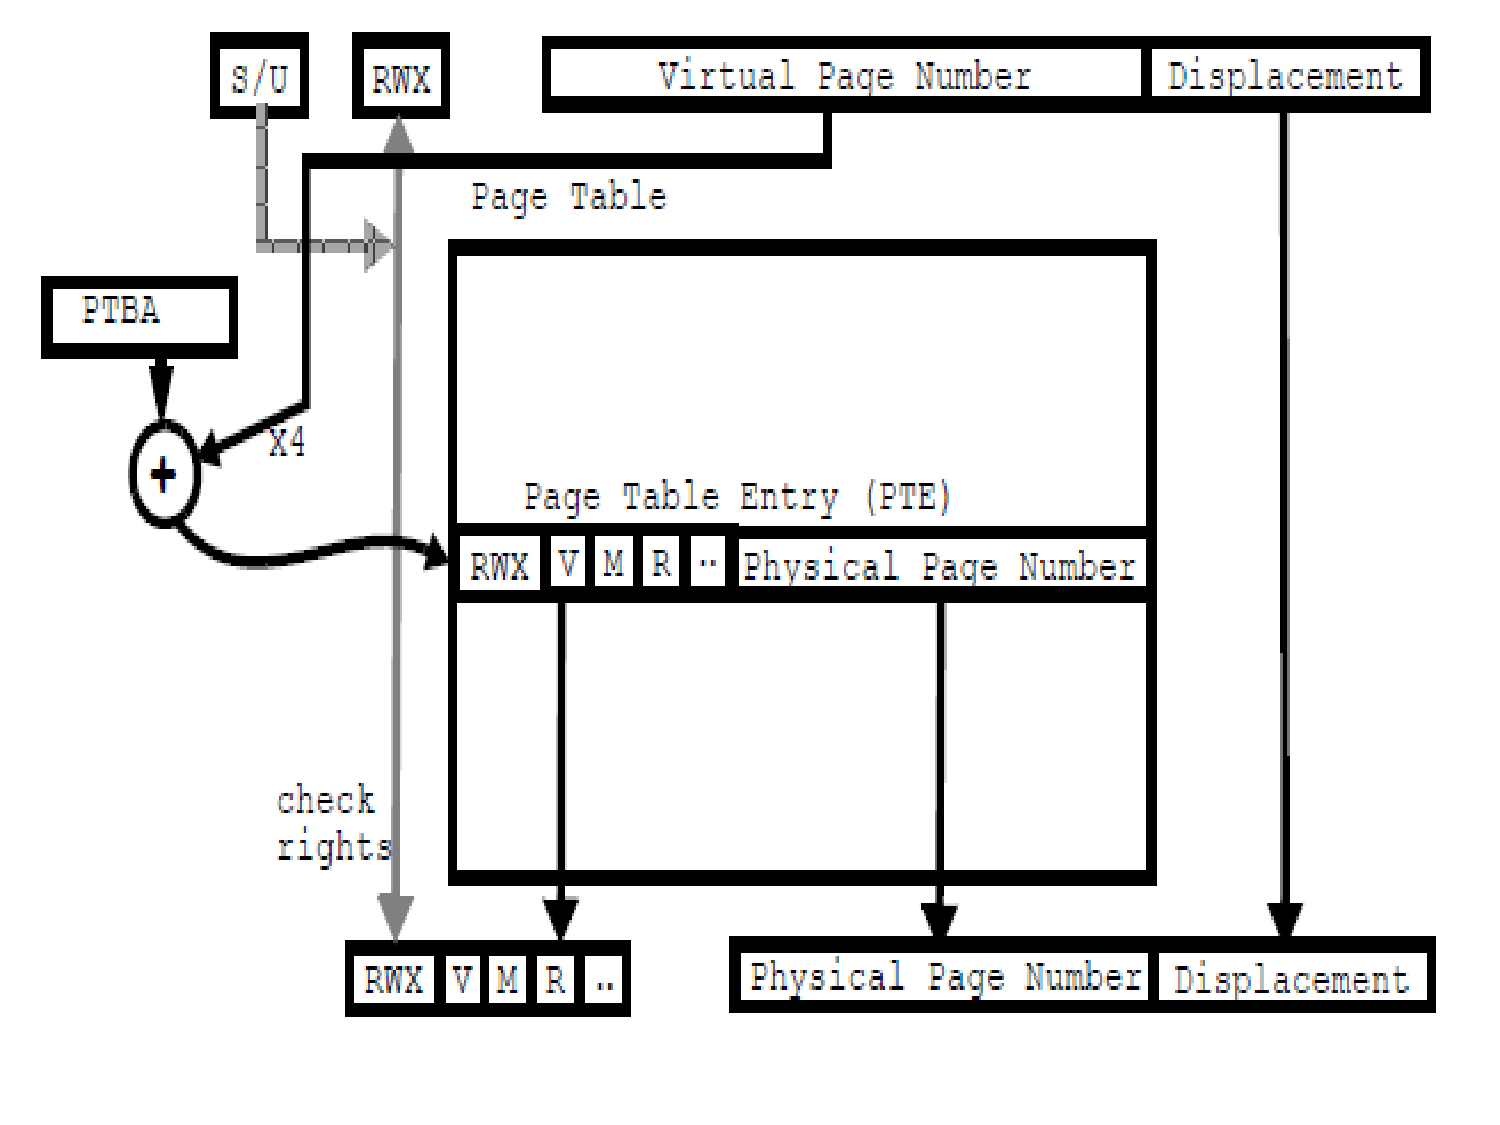
\includegraphics[width=40ex]{Figures/FigsMemH/PageTable}
\column{0.40\textwidth}
Translates Addresses \& Enforces Protection\smallskip

Page Replacement: FIFO--LRU--MFU
\end{columns}

Approximate LRU:
\begin{itemize}
\item Reference Bit (R) per page is periodically reset by OS.
\item Page Cached: hard vs soft page faults.
\end{itemize}\bigskip

Write-Back Strategy using Modify Bit (M);\\
M and R easily maintained by OS.

\end{frame}


\begin{frame}[fragile,t]
\frametitle{Hierarchical Page Table}

\begin{columns}
\column{0.55\textwidth}
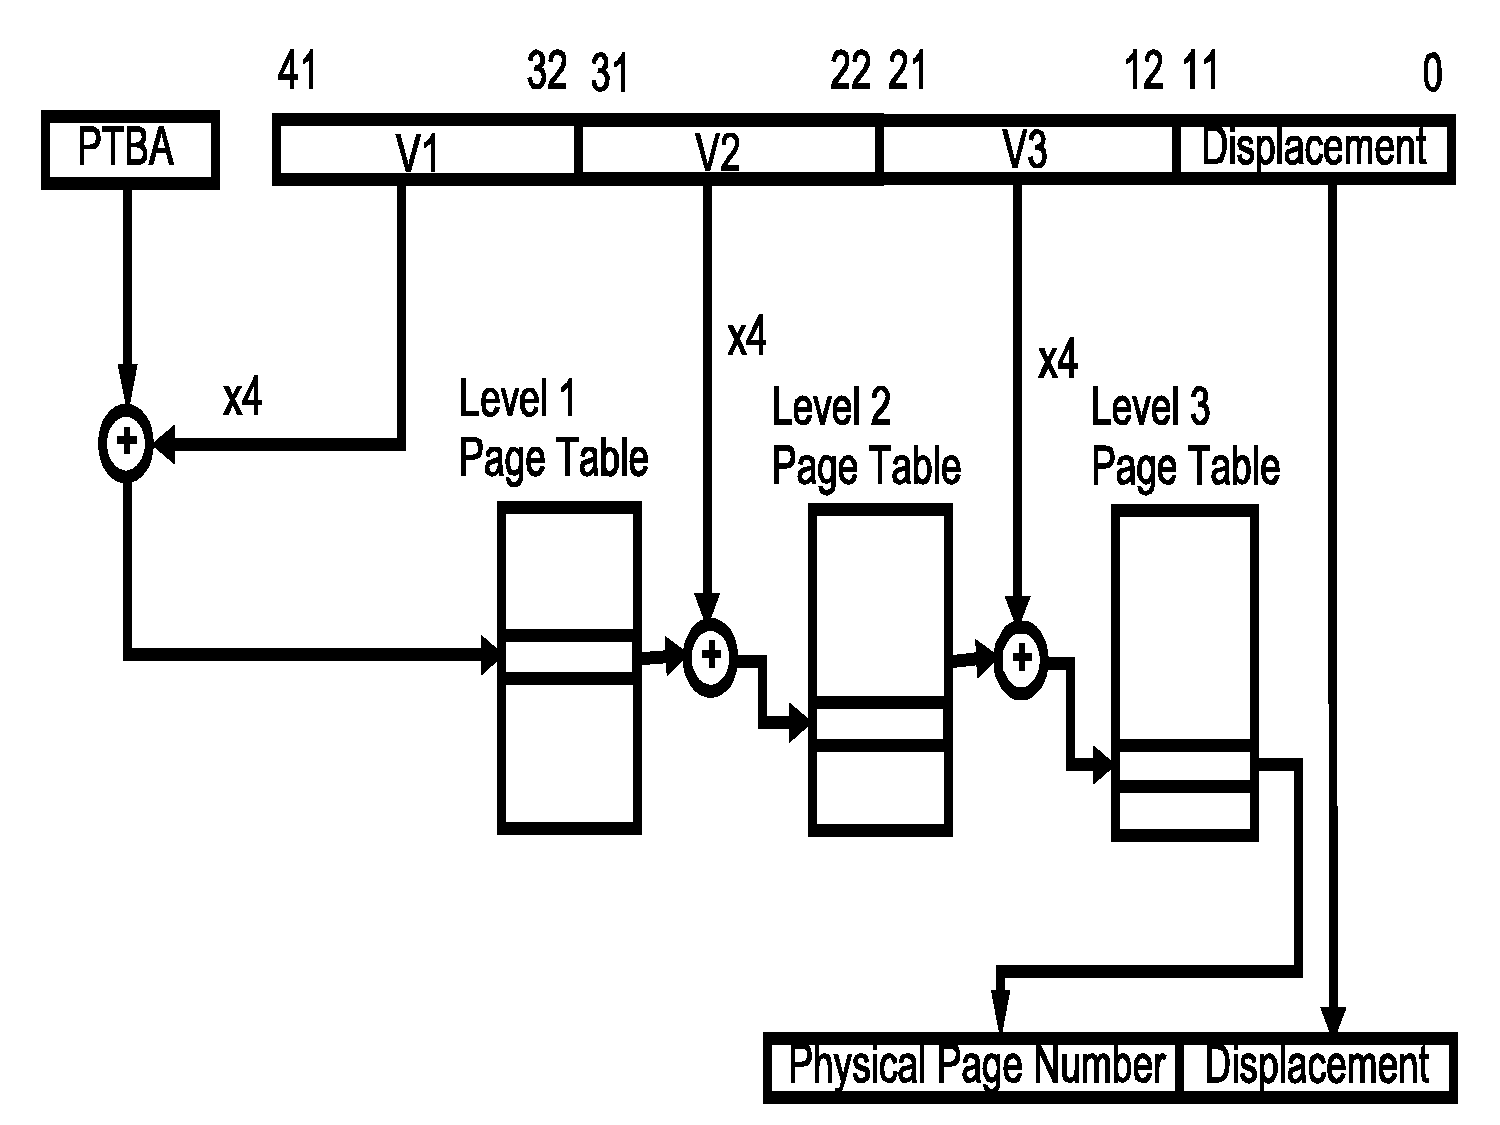
\includegraphics[width=40ex]{Figures/FigsMemH/HierarchPageTable}
\column{0.40\textwidth}
Supports SuperPages (How?)\smallskip


\end{columns}

Multiple DRAM access per memory translation:
\begin{itemize}
\item cached $\Rightarrow$ multiple cache accesses.
\item Solution: special cache dedicated to translations (TLB)
\end{itemize}\bigskip

\end{frame}

\begin{frame}[fragile,t]
\frametitle{Translation Lookahead Buffer (TLB)}

\begin{columns}
\column{0.55\textwidth}
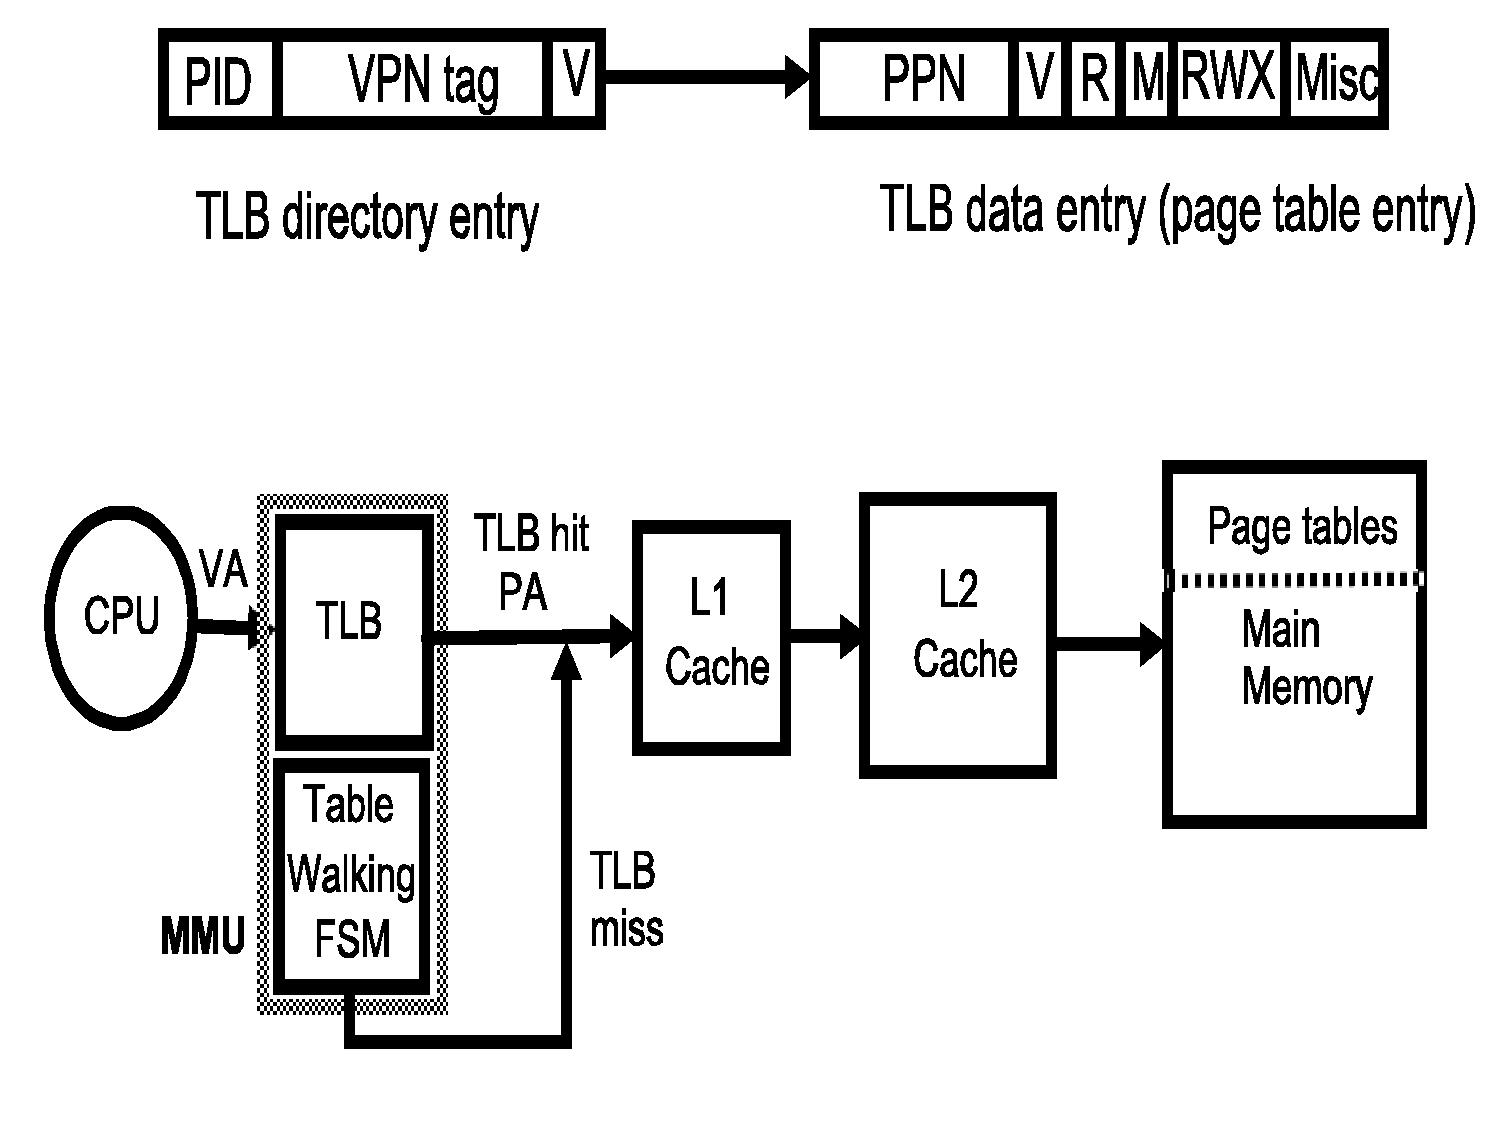
\includegraphics[width=40ex]{Figures/FigsMemH/TLB}
\column{0.40\textwidth}
Page Table Entries Are Cached in TLB:\\\smallskip
\begin{scriptsize}
TLB: DM/SA/FA cache accessed with VPN,\\
PID added to deal with homonyms.
\end{scriptsize}
\end{columns}

\begin{itemize}
\item TLBs $<<$ caches because of coverage.
\item iTLB and dTLB
\item TLB misses treated by ``table walking'' in 
\item Hardware MMU or software (trap handler).
\end{itemize}\bigskip

\end{frame}

\begin{frame}[fragile,t]
\frametitle{Optimizing TLB Access}

TLB is on the critical memory-access path:
\begin{itemize}
    \item pipeline: IF split into IF$_{TLB}$ \& IF$_{cache}$, same for ME stage
    \item access TLB in parallel with cache
        \begin{itemize}
            \item \emph{possible because of the two-step access}, but still
            \item \emp{L1 size is limited to 1 page per way of associativity. Why?}
        \end {itemize}
\end  {itemize}


\begin{columns}
\column{0.55\textwidth}
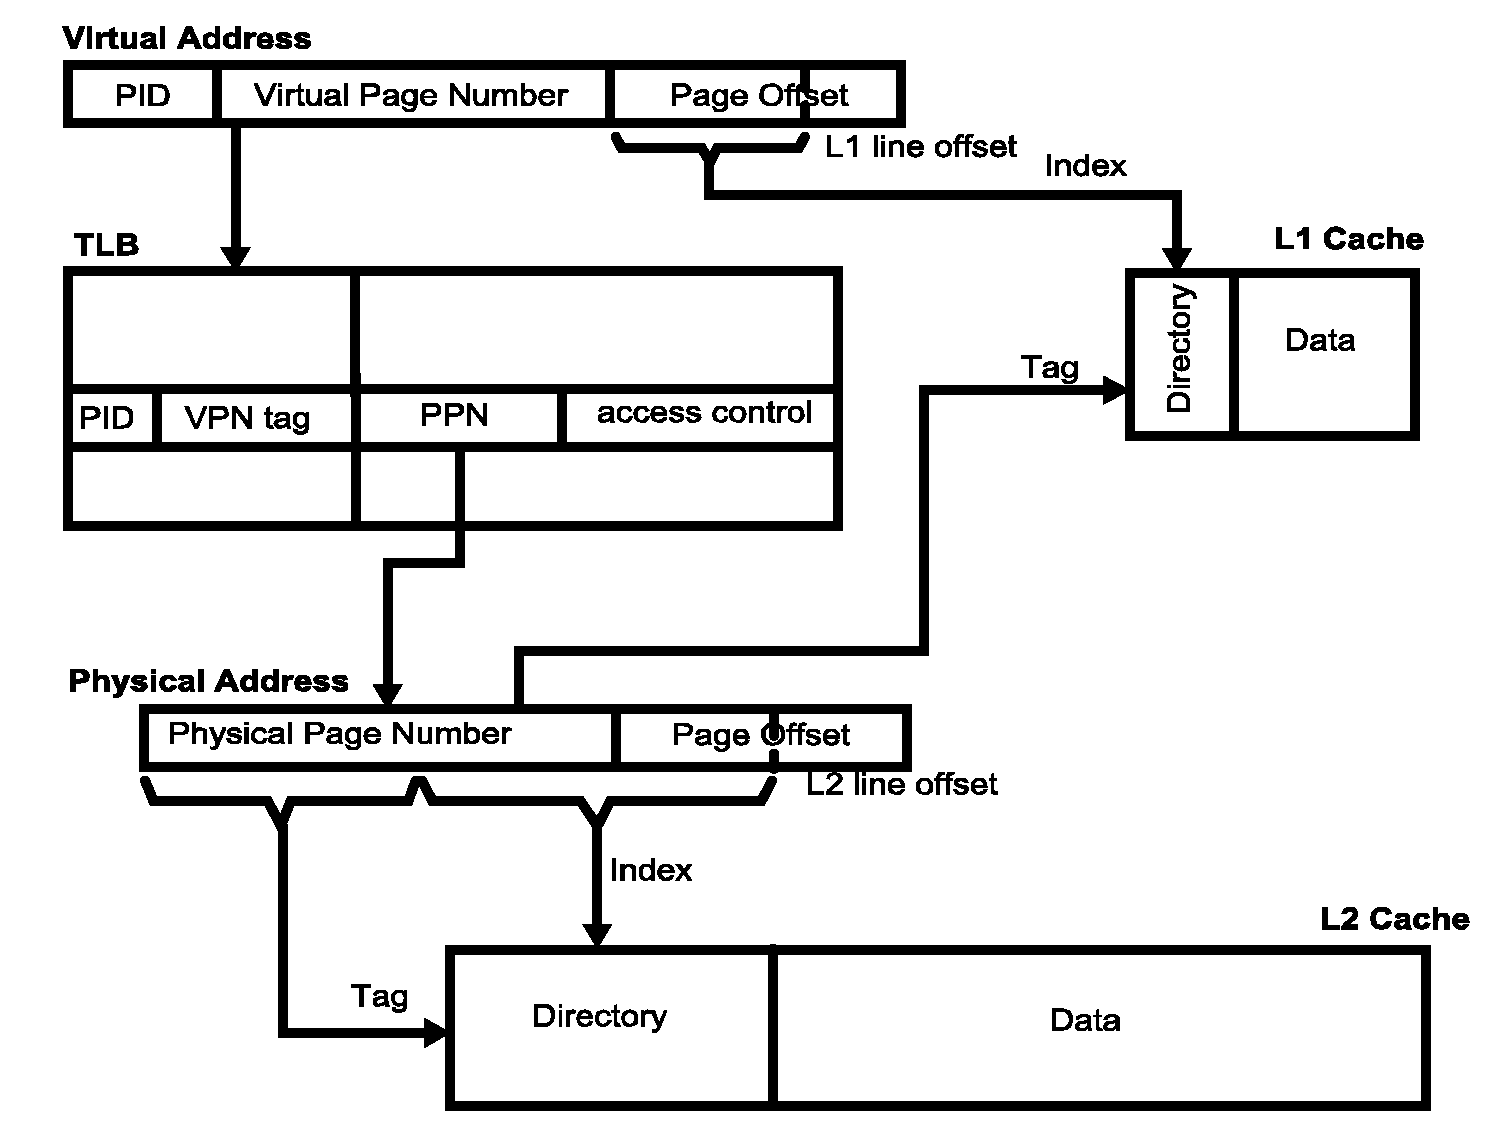
\includegraphics[width=40ex]{Figures/FigsMemH/TLBtransl}
\column{0.40\textwidth}
Need to use only bits in Page Offset to index in Directory.\\\bigskip

Otherwise: one block might be placed in two sets (due to synonyms).
\end{columns}

{\scriptsize Moving TLB after L1 cache, by indexing on the 
 virtual address $\Rightarrow$ many other problems!}

\end{frame}

%%%%%%%%%%%%%%%%%%%%%%%%%%%%%%%%%%%%%%%%%%%%%%%%%%%%%%
%%%%%%%%%%%%%%%%%%%%%%%%%%%%%%%%%%%%%%%%%%%%%%%%%%%%%%
%%%%%%%%%%%%%%%%%%%%%%%%%%%%%%%%%%%%%%%%%%%%%%%%%%%%%%
\section{Cache Coherence in Bus-Based Shared-Memory Multiprocessors}
\begin{frame}[fragile]
	\tableofcontents[currentsection]
\end{frame}

\begin{frame}[fragile,t]
\frametitle{Organization of Bus-Based Shared-Memory SMPs}

Design space of cache coherence for small scale SMPs 
assuming a broadcast-based interconnect, such as a bus.

\begin{columns}\hspace{-10ex}
\column{0.6\textwidth}
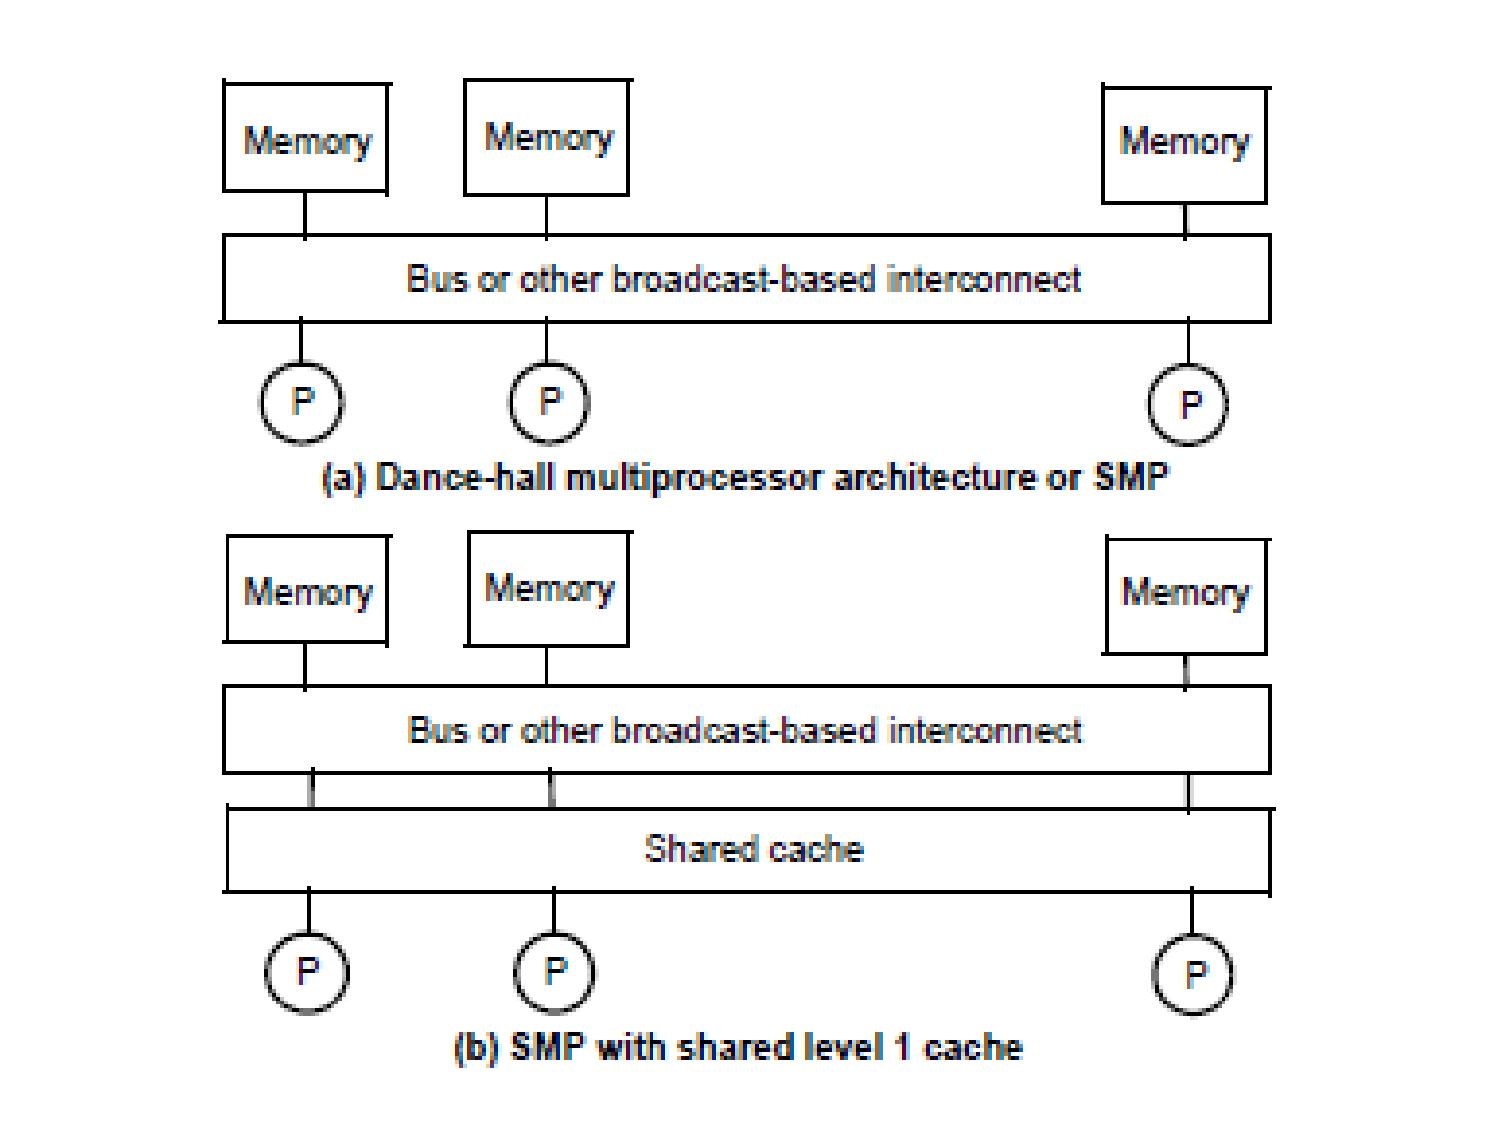
\includegraphics[width=50ex]{Figures/FigsInfCoherence/DanceHall}
\column{0.5\textwidth}\pause
        \begin{itemize}
        \begin{scriptsize}
            \item[\emp{(a)}] \emp{Dance-Hall}: implicit coherency\\but not realistic!
            \item Cache hierarchy vital for SMPs:
            \item hides memory \& interconnect latency,
            \item saves mem \& interconnect bandwidth.
        \end {scriptsize}
        \end  {itemize}
\bigskip
        \begin{itemize}
        \begin{scriptsize}
            \item[\emp{(b)}] \emp{Shared Cache} between processor \& interconnect:
            \item[\emph{+}] constructive sharing of cache resources.
            \item[\emp{--}] interconnect latency added to the critical 
                             mem access path $\Rightarrow$\\effective when very few processors.
        \end {scriptsize}
        \end  {itemize}
\end{columns}

\end{frame}

\begin{frame}[fragile,t]
\frametitle{Organization of Bus-Based Shared-Memory SMPs}

Design space of cache coherence for small scale SMPs 
assuming a broadcast-based interconnect, such as a bus.

\begin{columns}\hspace{-10ex}
\column{0.6\textwidth}
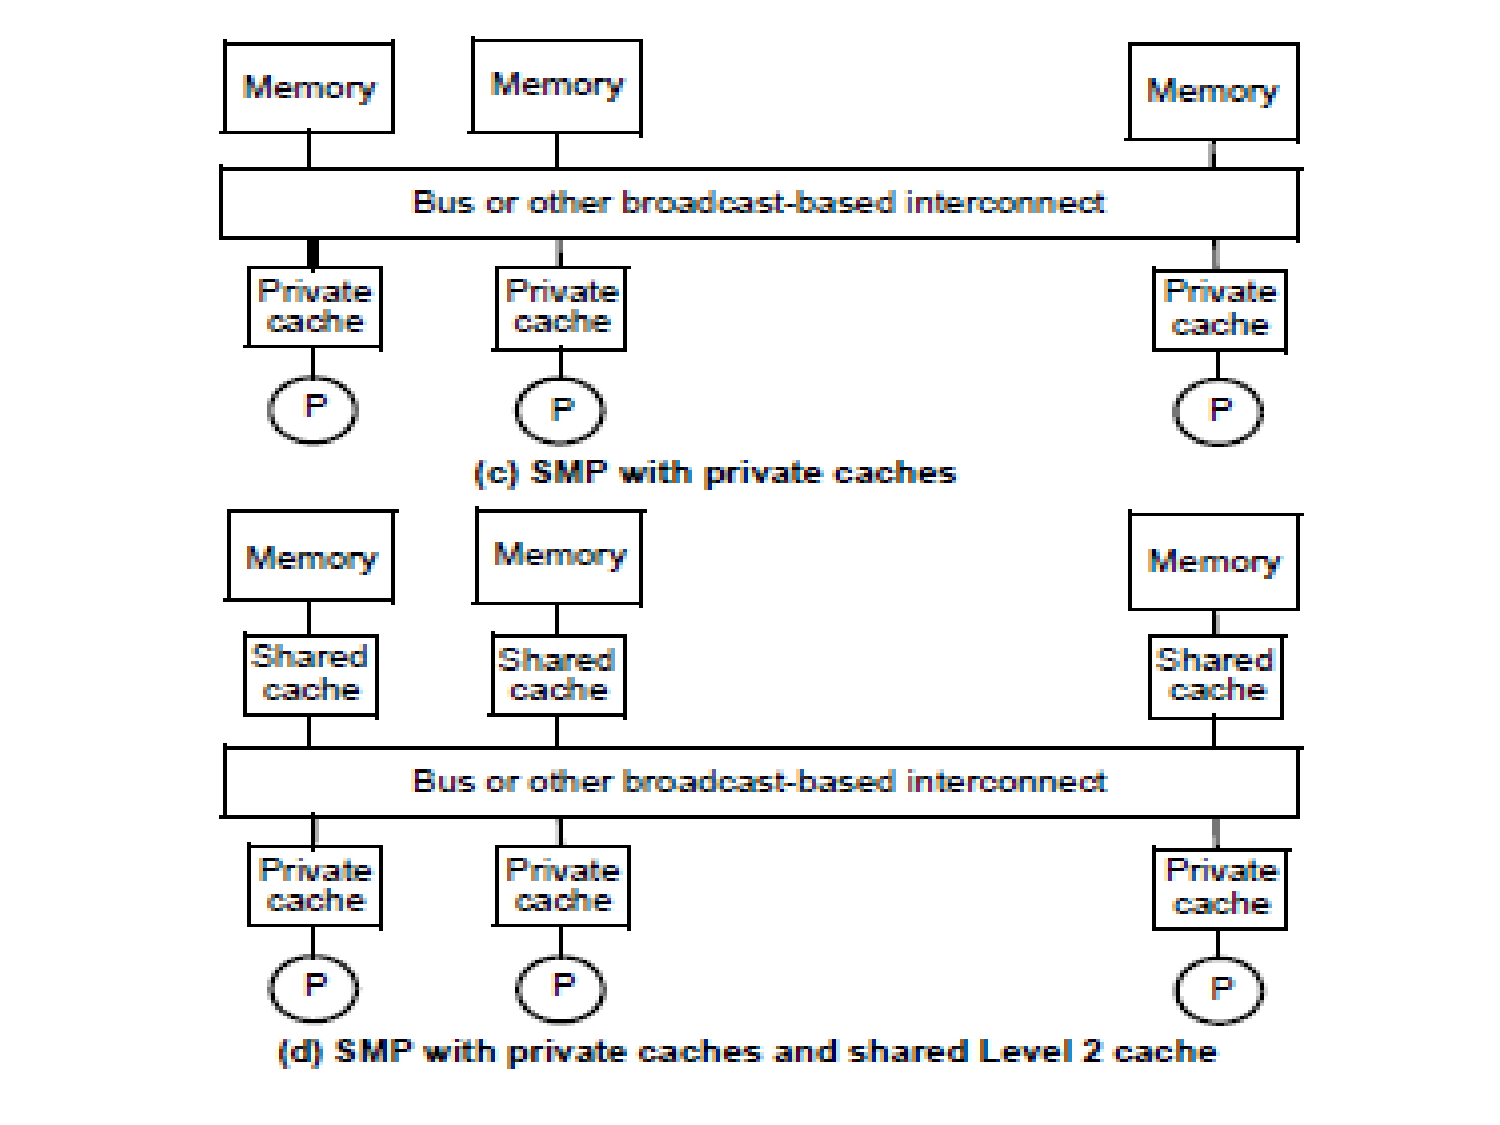
\includegraphics[width=50ex]{Figures/FigsInfCoherence/PrivCachSMP}
\column{0.5\textwidth}\pause
        \emp{(c) Private Cache on Proc Side}:
\bigskip
\bigskip
\bigskip

        \emph{(d) Hybrid Private-Shared Cache}:
        \begin{itemize}
        \begin{scriptsize}
            \item \emp{Private Cache} between processor \& interconnect:
            \item 2nd level cache (SLC) reduces memory access latency gap
                    between 1st level cache (FLC) and memory
            \item used in most commercially available processors.
        \end {scriptsize}
        \end  {itemize}
\end{columns}

\end{frame}

\begin{frame}[fragile,t]
\frametitle{Informal Definition of Cache Coherence}

\pause
\begin{definition}[Sequential Cache Coherence]
A load must return the value of the latest store 
in process order to the same address. (Simple, but check the write buffers.)
\end{definition}

\begin{definition}[Cache Coherence in Multiprocessors]
A cache system is cache coherent {\em iff} all processors, 
at any time, have a consistent view of the last 
globally written value to each location.
\end{definition}

\medskip

\alert{Coherence Problem: pervasive \& performance critical}
\begin{scriptsize}
\begin{itemize}
    \item sharing of data, implicit communication, 
    \item thread migration, software not informed $\Rightarrow$ hardware must solve the problem.
\end  {itemize}
\end {scriptsize}

\end{frame}


\begin{frame}[fragile,t]
\frametitle{Locking, Barrier, Point-to-Point Synchronization}

\begin{block}{Barrier and {\tt~~~~~~~~~~~~~~~~~~} Point-to-Point Synchronization}
\begin{columns}
\column{0.21\textwidth}
\begin{colorcode}[fontsize=\scriptsize]
\mymath{T\myindx{1}}
...
BAR := BAR + 1 
while( BAR < 2 ) ;
...
\end{colorcode} 
\column{0.21\textwidth}
\begin{colorcode}[fontsize=\scriptsize]
\mymath{T\myindx{1}}
...
BAR := BAR + 1 
while( BAR < 2 ) ;
...
\end{colorcode} 
\column{0.25\textwidth}
\begin{colorcode}[fontsize=\scriptsize]
\mymath{T\myindx{1}}


while( FLAG == 0 ) ;
print A
\end{colorcode} 
\column{0.18\textwidth}
\begin{colorcode}[fontsize=\scriptsize]
\mymath{T\myindx{2}}
A    := 1;
FLAG := 1;


\end{colorcode} 
\end{columns}
\end{block}
\medskip

\emp{Point-to-Point}: no need for critical section; producer-consumer sync.
\medskip

\emp{Barrier}: all threads have to reach it before executing beyond it.
\begin{itemize}
    \item \alert{need critical section to increment {\tt BAR}} + \emph{read/reset {\tt BAR} fine}.
    \item but even assuming the writes to bar do not interleave, i.e., atomic,
            with the current cache design:\pause
    \begin{itemize}
    \item[write back:] P1 and P2 write {\tt M}, then barrier, then both
        read {\tt M} $\Rightarrow$\\
        if cache line not evicted, both read their private-cache value.\smallskip
    \item[write through:] P1 writes {\tt M} (mem updated), then P2 writes {\tt M}, barrier 
        $\Rightarrow$\\P1 will read an inconsistent value next from its private cache.
    \end  {itemize}
\end  {itemize}

\alert{Need Coherence!}

\end{frame}

\subsection{Simple Protocol for Write-Through Caches}

\begin{frame}[fragile,t]
\frametitle{Simple Protocol For Write-Through Caches}

Simplifying Assumptions:
\begin{scriptsize}
\begin{itemize}
    \item blocking, write-through, write-allocate, single-level private cache as in (c) 
    \item when granted access, cache controller owns the bus until transaction completes.
\end  {itemize}
\end {scriptsize}
\smallskip

\begin{columns}
\column{0.5\textwidth}
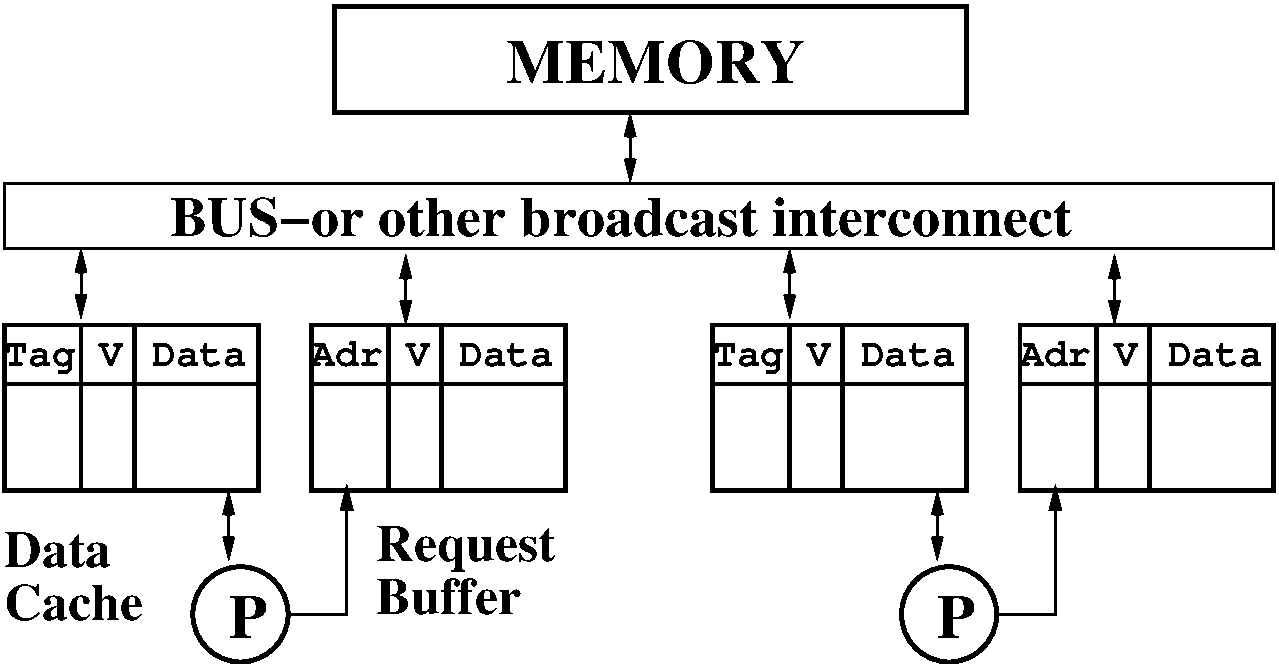
\includegraphics[width=35ex]{Figures/FigsInfCoherence/SMPreqbuff}
\column{0.45\textwidth}\pause
Local cache updated last:\\
\emp{``last globally written value''
cannot be released until all
other procs can see the new value}.
\end{columns} 

\smallskip
%\begin{scriptsize}
\begin{itemize}
    \item[Rd Miss] inserted in (request) buffer, V(alid) bit set.
    When bus acquired $\Rightarrow$ {\tt BusRd} request placed on bus \& returns copy of mem block.\pause

    \item[Wr Hit:] value and address inserted in buffer. \pause When acquired, 
    {\tt BusWrite} request on bus $\Rightarrow$ updates memory AND \alert{invalidates all
    remote copies} (clears V). \emp{Local cache updated just before releasing bus.}

    \item[Wr Miss] like Wr Hit, but {\tt BusRdX} on bus (also brings block from mem).
    For no-write-allocate: like WR Hit, but local cache not updated.

\end  {itemize}
%\end {scriptsize}

\end{frame}

\begin{frame}[fragile,t]
\frametitle{Specify Behavior via Finite State Machine (FSM)}

%%Assumptions: no-allocate on store miss, all store and loads propagate on bus,
%% store may update or invalidate caches.

Each cache represented by a FST:
\begin{itemize}
    \item Imagine P identical FSM working together (one per cache), 
    \item Actually, FSM shows the cache behavior w.r.t. a memory block.
    \item 2 states: Valid or Invalid (not in cache), requires 1 bit (V)
\end  {itemize}
\bigskip

For example a write (hit) in valid state remains in valid, but
triggers a {\tt BusWrite} which may cause other caches to transition
to invalid. 

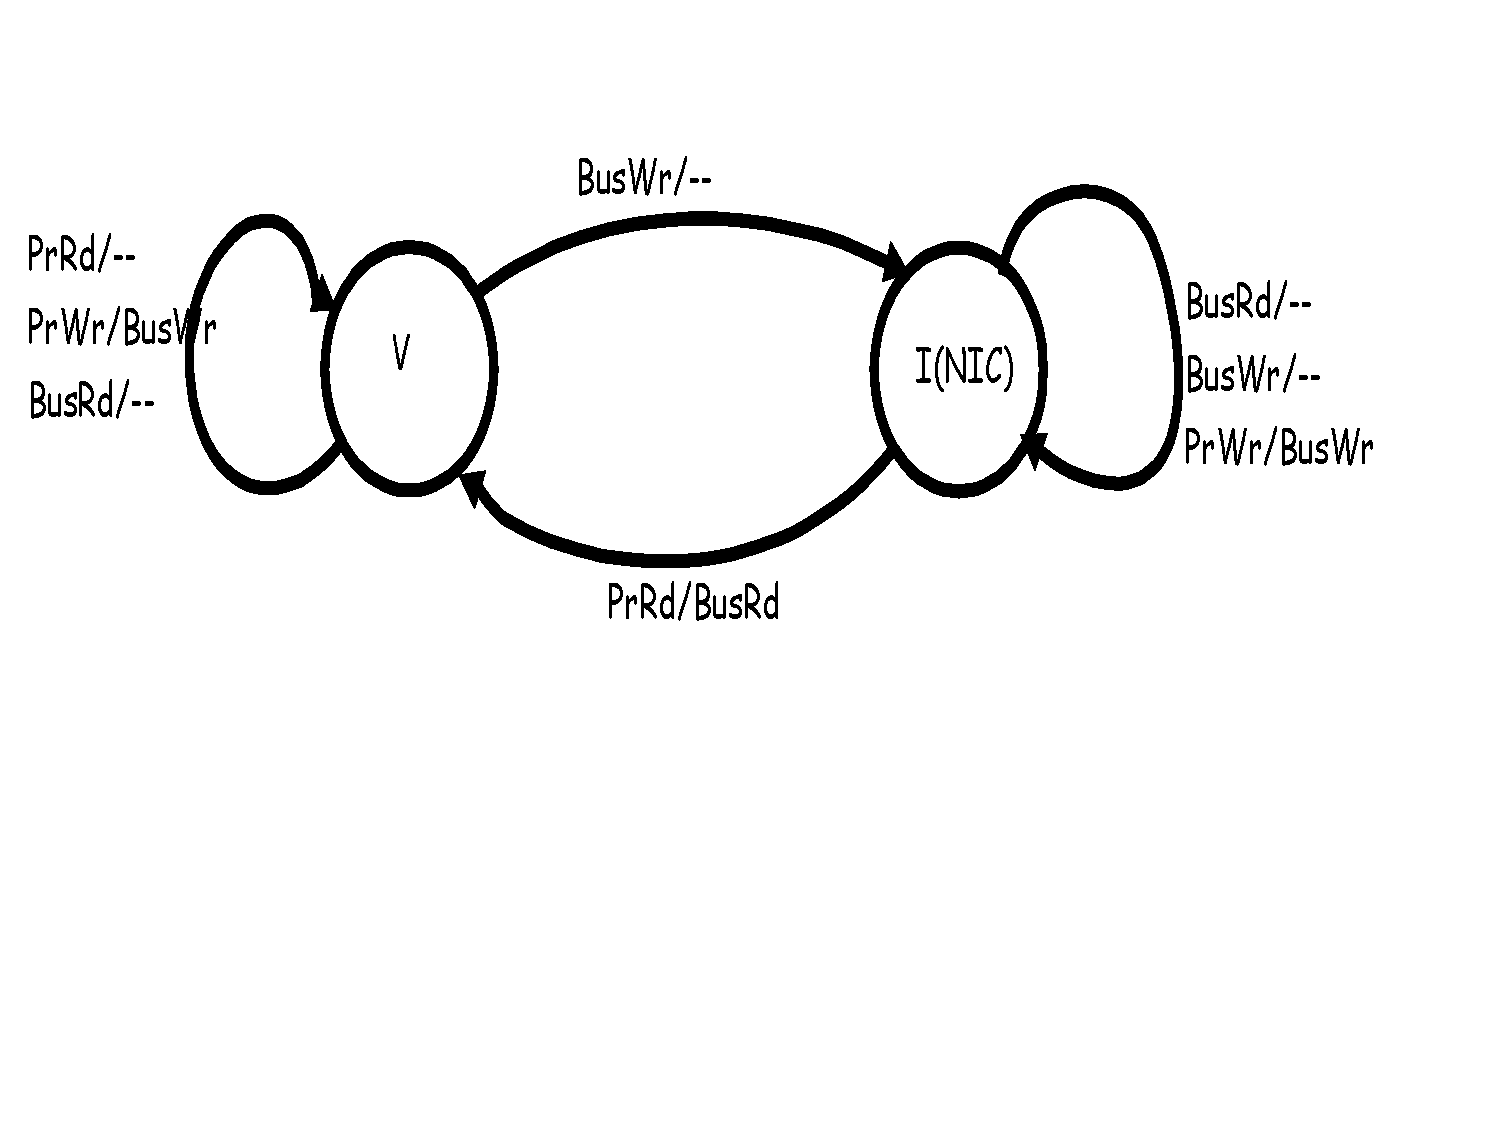
\includegraphics[width=59ex]{Figures/FigsInfCoherence/SimpleCohProt}

\end{frame}



\begin{frame}[fragile,t]
\frametitle{Copy Invalidation By Bus Snooping}


%\begin{scriptsize}
\begin{itemize}
    \item Bus interface can monitor (snoop) traffic \& 
    \item if tag matches $\Rightarrow$ invalidate (local) cache entry (clear V).
\end  {itemize}
%\end {scriptsize}
\smallskip

\begin{columns}
\column{0.5\textwidth}
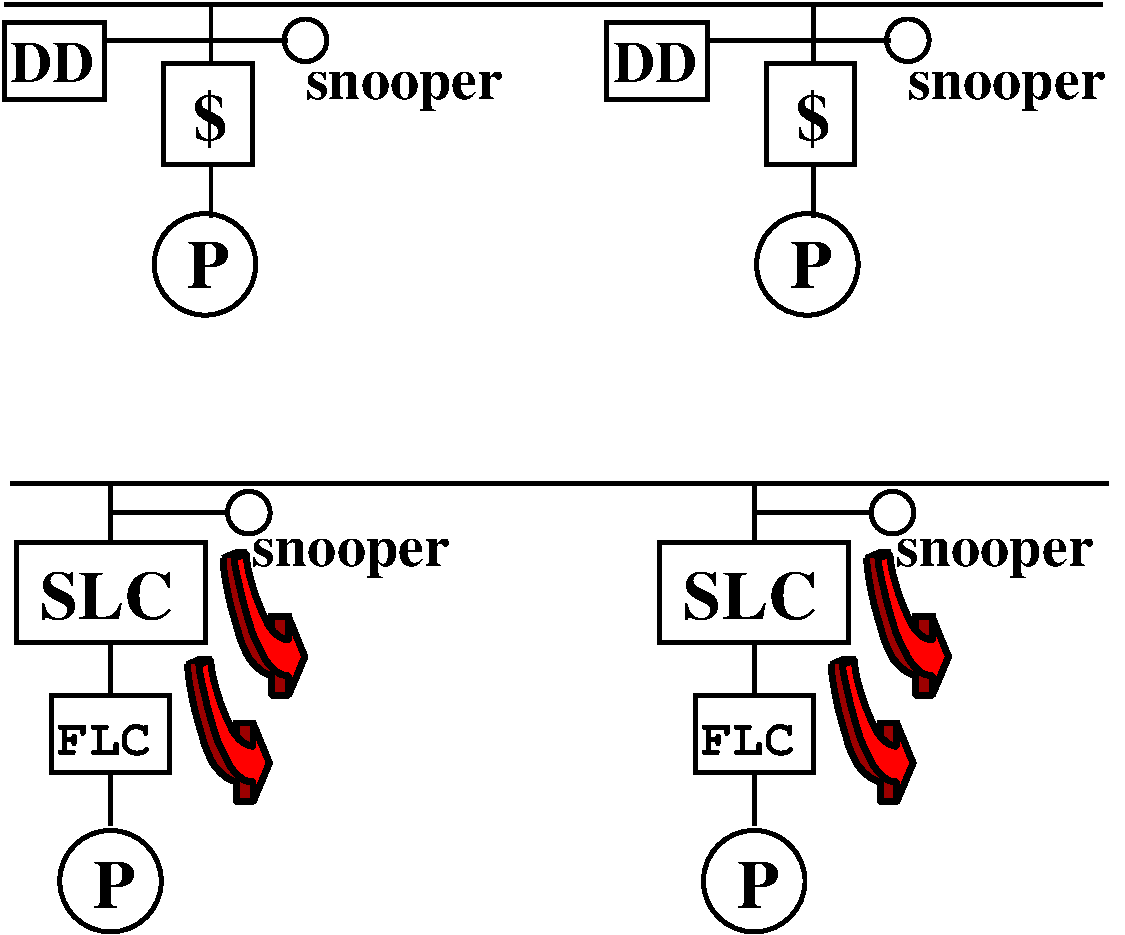
\includegraphics[width=35ex]{Figures/FigsInfCoherence/SnoopingEg}
\column{0.45\textwidth}\pause
\emp{Dual Directory (DD)} is a copy of cache directory,
kept consistent on updates (rare).

DD filters out bus requests to avoid conflicts with CPU.

\bigskip
Inclusion $\Rightarrow$ \emp{SLC} contains bit indicating whether block is in FLC,
and is used to \emp{filter out transactions from FLC}
(since SLC far less busy than FLC) 
\end{columns} 

\smallskip
%\begin{scriptsize}
%\begin{itemize}
%\end  {itemize}
%\end {scriptsize}

\end{frame}

\begin{frame}[fragile,t]
\frametitle{Example of Subtle Issue}

\begin{columns}
\column{0.48\textwidth}
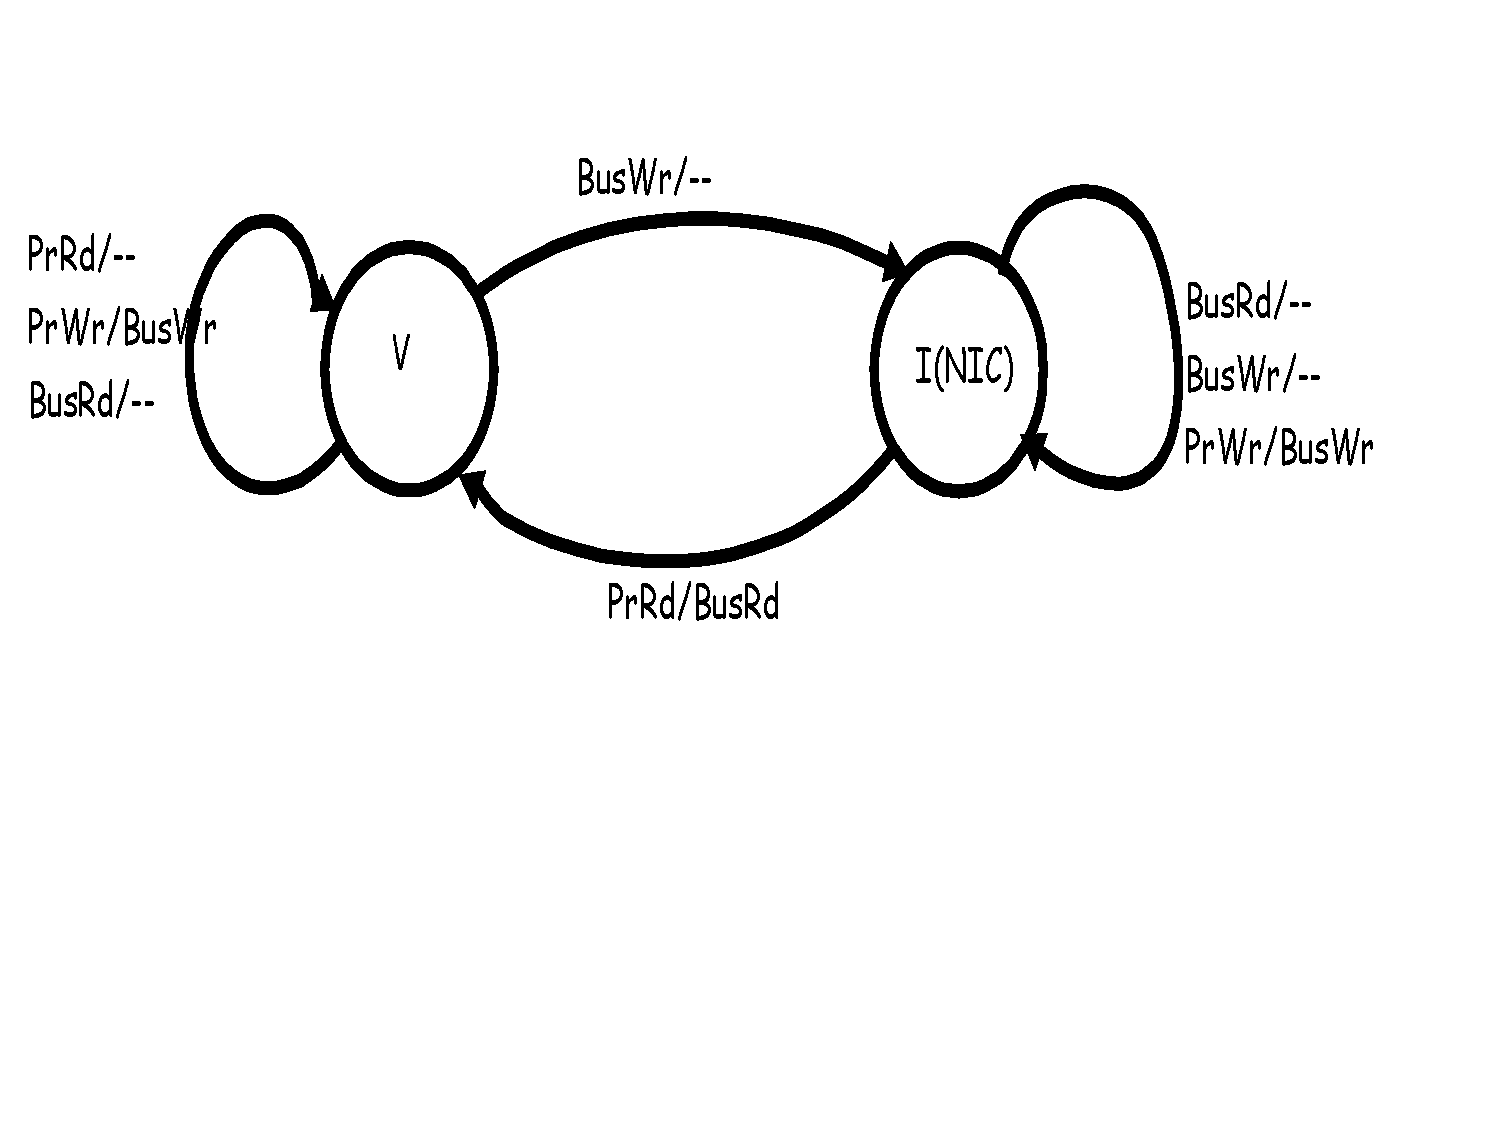
\includegraphics[width=35ex]{Figures/FigsInfCoherence/SimpleCohProt}
\column{0.48\textwidth}
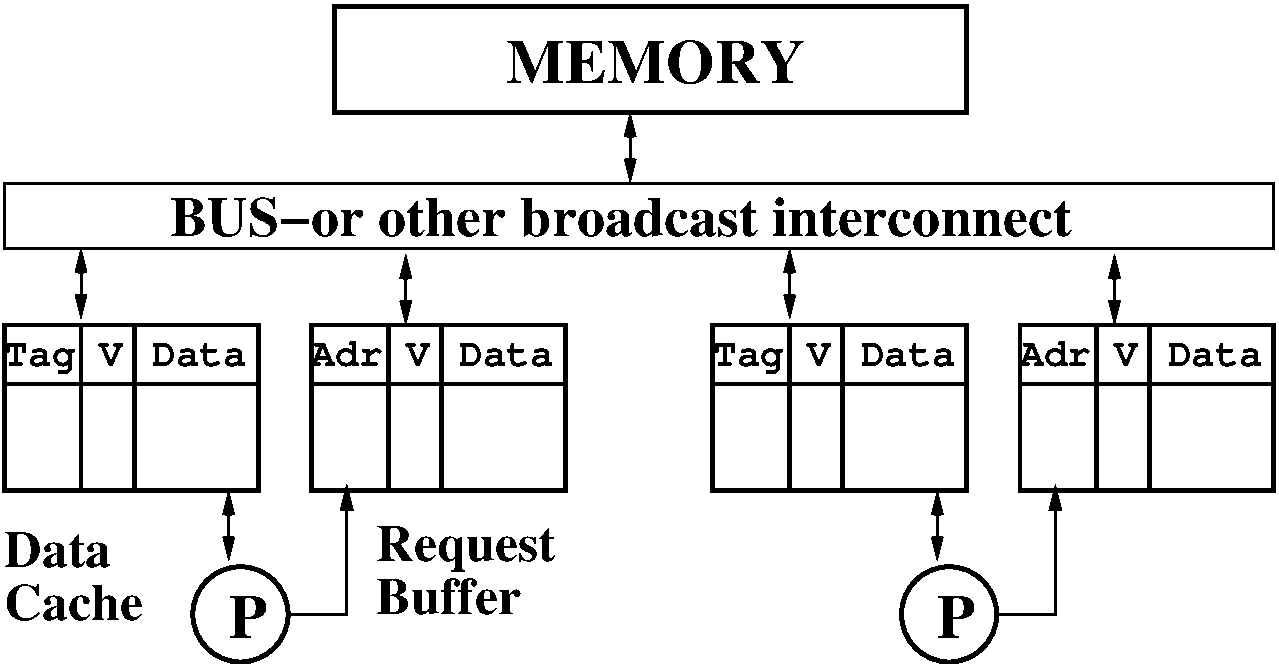
\includegraphics[width=30ex]{Figures/FigsInfCoherence/SMPreqbuff}
\end{columns}
\vspace{-3ex}
FST specifies the \emp{high-level} behavior of cache as a whole.\\
\emp{The use of request buffer is not safe, and will be fixed later.}
%\begin{scriptsize}
\begin{itemize}
    \item P1 and P2 issue \emp{write hits} to block A. 
    \item Assume P1 acquire bus while P2 waits in buffer. \alert{What happens?}\pause
    \item P1 issues a \emp{\tt BusWrite}, which invalidates the P2's cache $\Rightarrow$
    \item When P2 acquires bus, it has to check V bit in cache, and send a \emp{\tt BusRdX},
            rather than {\tt BusWrite} request.
\end{itemize}

\end{frame}


\subsection{Design Space: MSI, MESI, MOESI Protocols}

\begin{frame}[fragile,t]
\frametitle{MSI Protocol for Write Back Caches}

Simple Protocol suffers performance bottlenecks:
\begin{itemize}
    \item \alert{All writes launch bus transactions.}\pause
    \item \emph{Key Insight}: most blocks accessed exclusively
            by one processor $\Rightarrow$ accesses to non-shared 
            block cannot interfere with other caches!
\end{itemize} 


\begin{columns}\hspace{-7ex}
\column{0.43\textwidth}
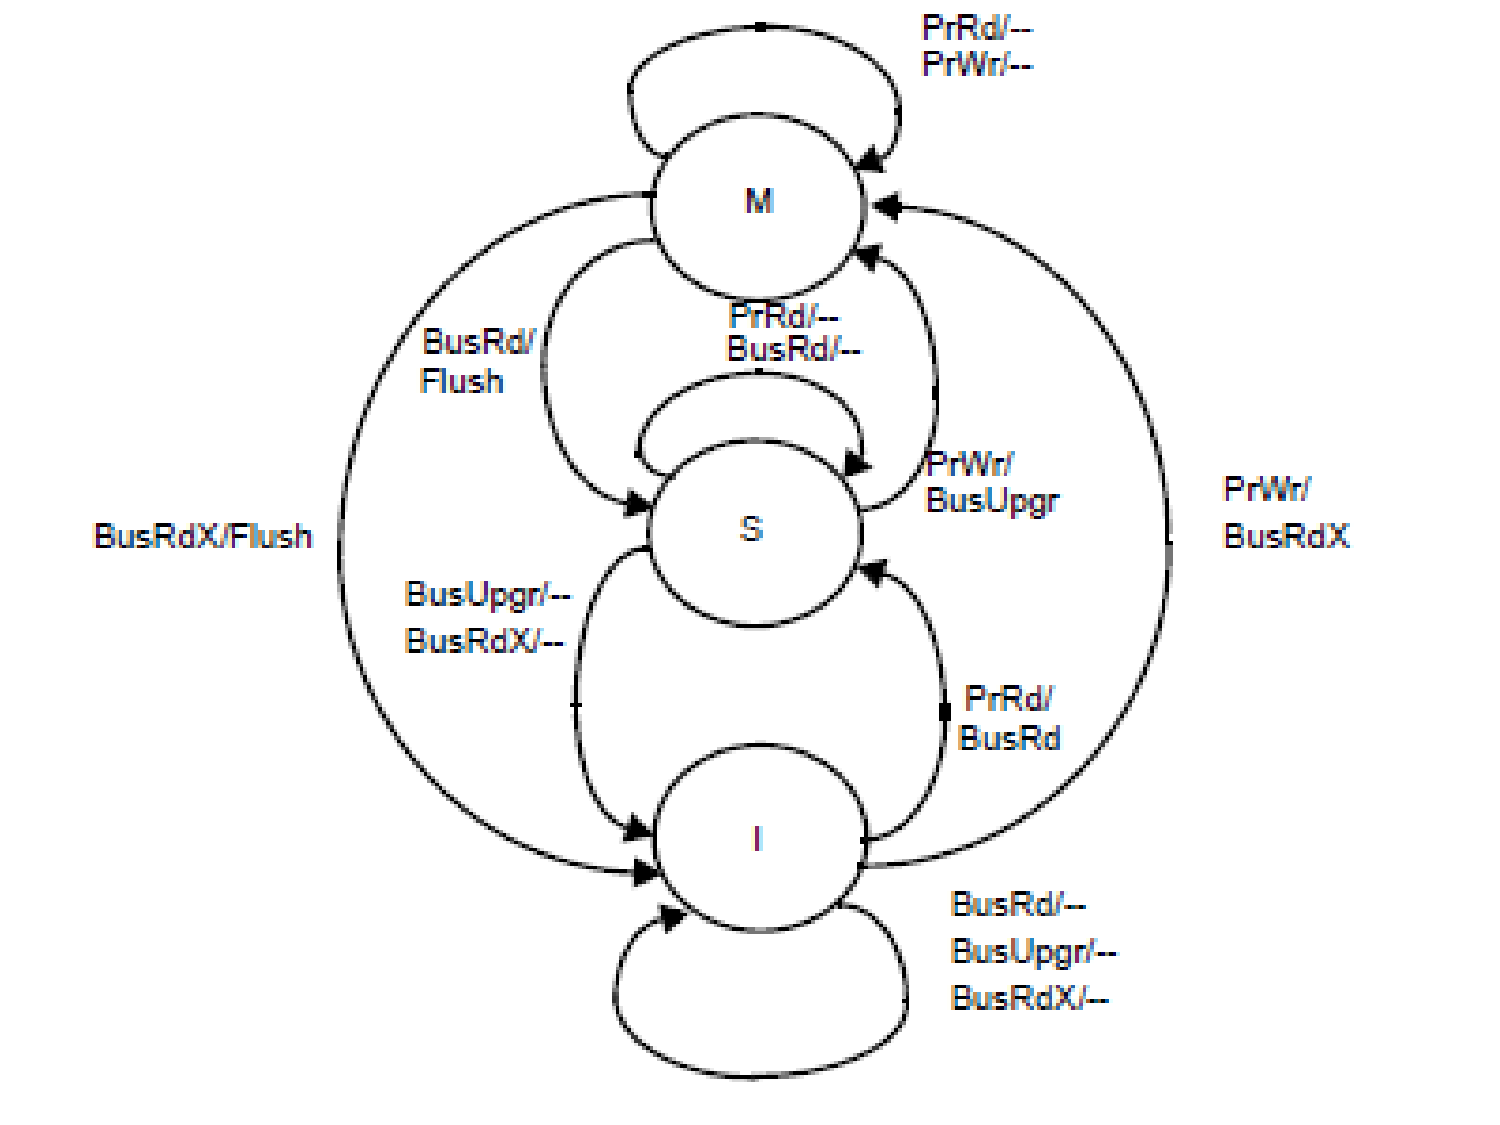
\includegraphics[width=40ex]{Figures/FigsInfCoherence/MSI}\pause
\column{0.55\textwidth}
\begin{scriptsize}
\begin{itemize}
    \item State V split into M(odified) \& S(hared):\smallskip
    \item[M] local copy is the only up-to-date one,\\
            read \& writes performed locally!\\
            (Extra state bit M for write-back cache.)\smallskip
    \item[S] several remote copies available \& all copies in S and memory are up-to-date!\\
             Reads operate locally, but a write must invalidate 
            all remote copies (via {\tt BusUpgr}).\smallskip
    \item[I] local copy invalid or not in cache.\\
                \emp{Who provides the value on a read miss?}\\
                    \emp{If exists}, {\bf necessarily} by a remote copy in M;\\ 
                    Operation named {\tt Flush}: forward block\\ 
                    copy to requester \& also update memory.\\
                    \emp{Otherwise}, either by a copy in S or mem.
\end{itemize}
\end{scriptsize}
\end{columns}

\end{frame}


\begin{frame}[fragile,t]
\frametitle{MSI Protocol: Examples}

\begin{itemize}
    \item \emph{\tt BusRd} requests a copy with no intent to modify.
    \item \emph{\tt BusRdX} requests a copy with intent to modify (and invalidates remote copies).
    \item \emph{\tt BusUpgr} invalidate remote copies.  
    \item \emph{\tt Flush} forward copy to requester \& update memory.
\end{itemize} 


\begin{columns}\hspace{-7ex}
\column{0.43\textwidth}
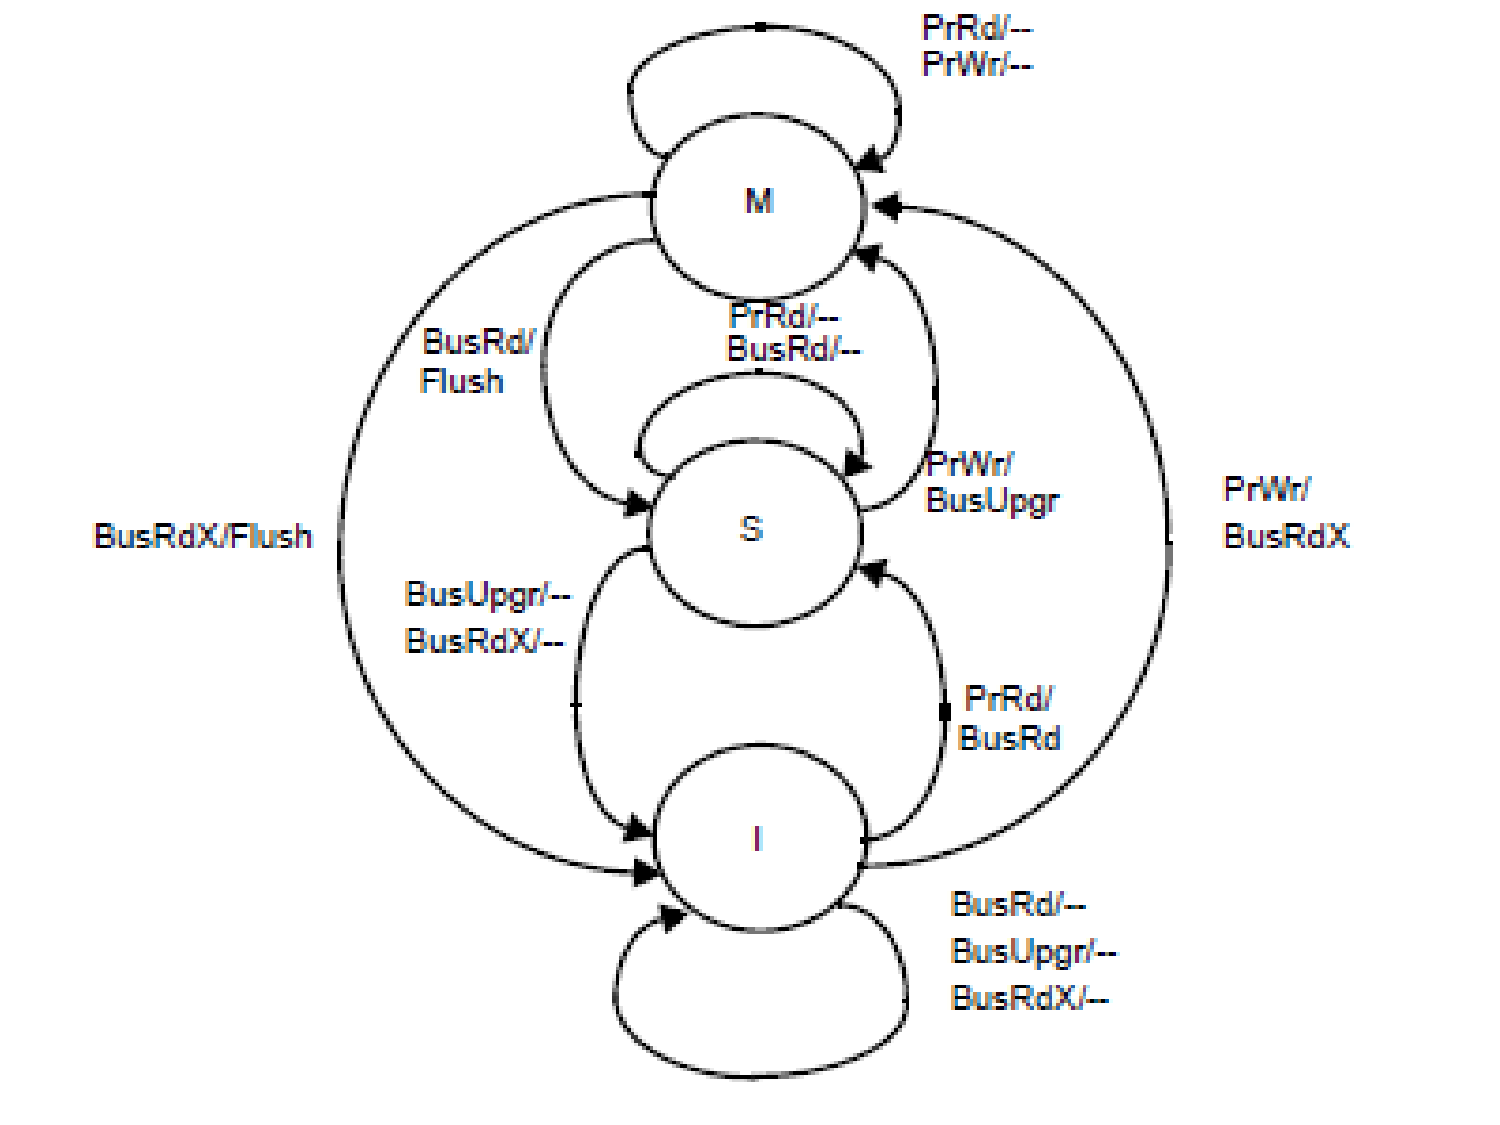
\includegraphics[width=40ex]{Figures/FigsInfCoherence/MSI}
\column{0.55\textwidth}
\begin{scriptsize}
\begin{itemize}
    \item[1] \emph{Assume block A not in any cache:}
    \item P reads A: 
    \item P writes A:  
    \item Next reads \& writes of P:\medskip

    \item[2] \emph{Assume only $P_i$ and $P_j$ have S copies.}
    \item[$P_i$ writes] {\tt~~}\\
                        {\tt~~}
    \item[$P_j$ reads.] {\tt~~}\\
                        {\tt~~}\\
                        {\tt~~}
    \item[$P_k$ reads.] {\tt~~}\\
                        {\tt~~}\\ 
                        {\tt~~}\\
\end{itemize}
\end{scriptsize}
\end{columns}

\end{frame}

\begin{frame}[fragile,t]
\frametitle{MSI Protocol: Examples}

\begin{itemize}
    \item \emph{\tt BusRd(X)} requests copy with (no) intent to modify.
    \item \emph{\tt BusUpgr} invalidate remote copies.  
    \item \emph{\tt Flush} forward copy to requester \& update memory.
\end{itemize} 


\begin{columns}\hspace{-7ex}
\column{0.43\textwidth}
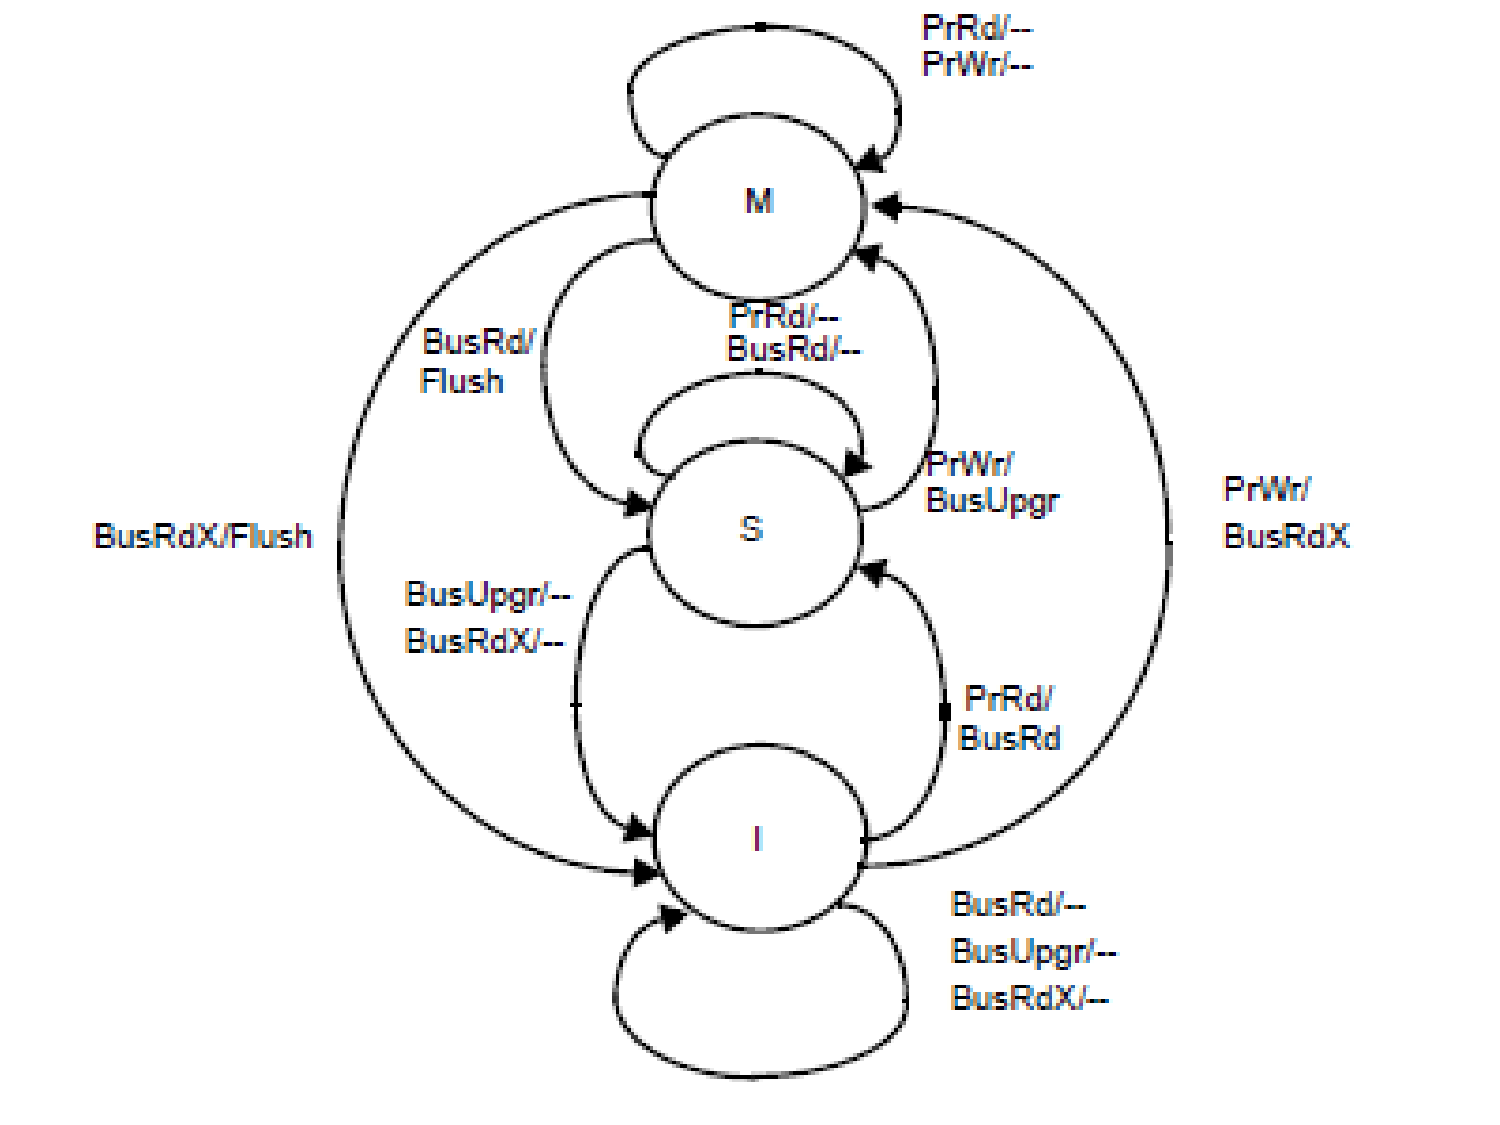
\includegraphics[width=40ex]{Figures/FigsInfCoherence/MSI}
\column{0.55\textwidth}
\begin{scriptsize}
\begin{itemize}
    \item[1] \emph{Assume block A not in any cache:}
    \item P reads A: I $\rightarrow$ S
    \item P writes A: S $\rightarrow$ M and launches {\tt BusUpgrd} to invalidate remote copies,  
    \item Next reads \& writes of P: execute locally.\medskip

    \item[2] \emph{Assume only $P_i$ and $P_j$ have S copies:}
    \item[$P_i$ writes] $P_i$: S $\rightarrow$ M and launches {\tt BusUpgr},\\
                        on which $P_j$: S $\rightarrow$ I
    \item[$P_j$ reads.]  $P_j$: I $\rightarrow$ S and launches {\tt BusRd},\\
                         on which $P_i$: M $\rightarrow$ S and flushes its\\
                        (only up-to-date) copy to $P_j$ and memory.
    \item[$P_k$ reads.] $P_k$: I $\rightarrow$ S and launches {\tt BusRd},\\
                        and the value is brought from memory.\\ 
                        All copies are in state S.
\end{itemize}
\end{scriptsize}
\end{columns}

\end{frame}


\begin{frame}[fragile,t]
\frametitle{MSI: Hardware Structures}

\begin{columns}\hspace{-5ex}
\column{0.6\textwidth}
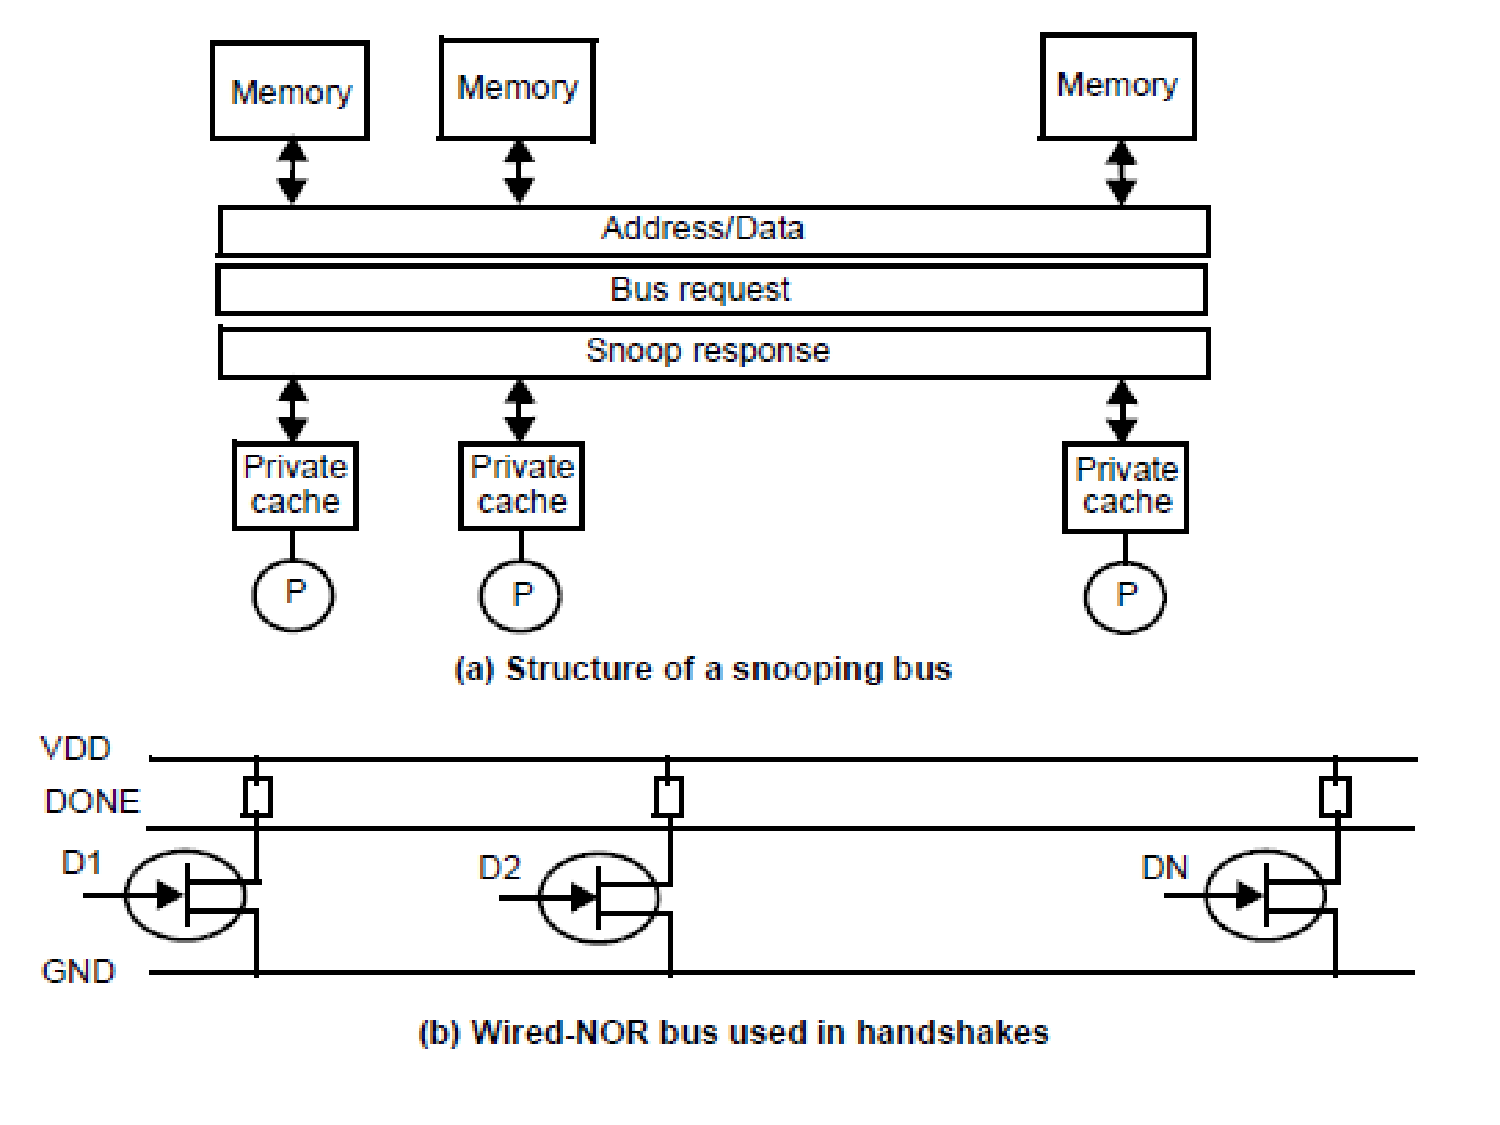
\includegraphics[width=47ex]{Figures/FigsInfCoherence/SnoopingBus}
\column{0.45\textwidth}
\vspace{-3ex}
\begin{scriptsize}
\begin{itemize}
    \item Transaction starts by supplying \emp{address/data} and a \emp{request}.
    \item and triggers a \emp{snoop action}, e.g., invalidate tag, and \emp{reply},
            e.g., when have all completed it?
    \item \emp{Synchronous} reply:  
    \item \emp{Asynchronous} by handshake (b):\\{{\tt NOR(D1,..,Dn)$\Rightarrow$ DONE}}, i.e.,\\
    \item \emp{Fetch from Remote or Memory?}
\end{itemize}
\end{scriptsize}
\end{columns}

\end{frame}

\begin{frame}[fragile,t]
\frametitle{MSI: Hardware Structures}

\begin{columns}\hspace{-5ex}
\column{0.6\textwidth}
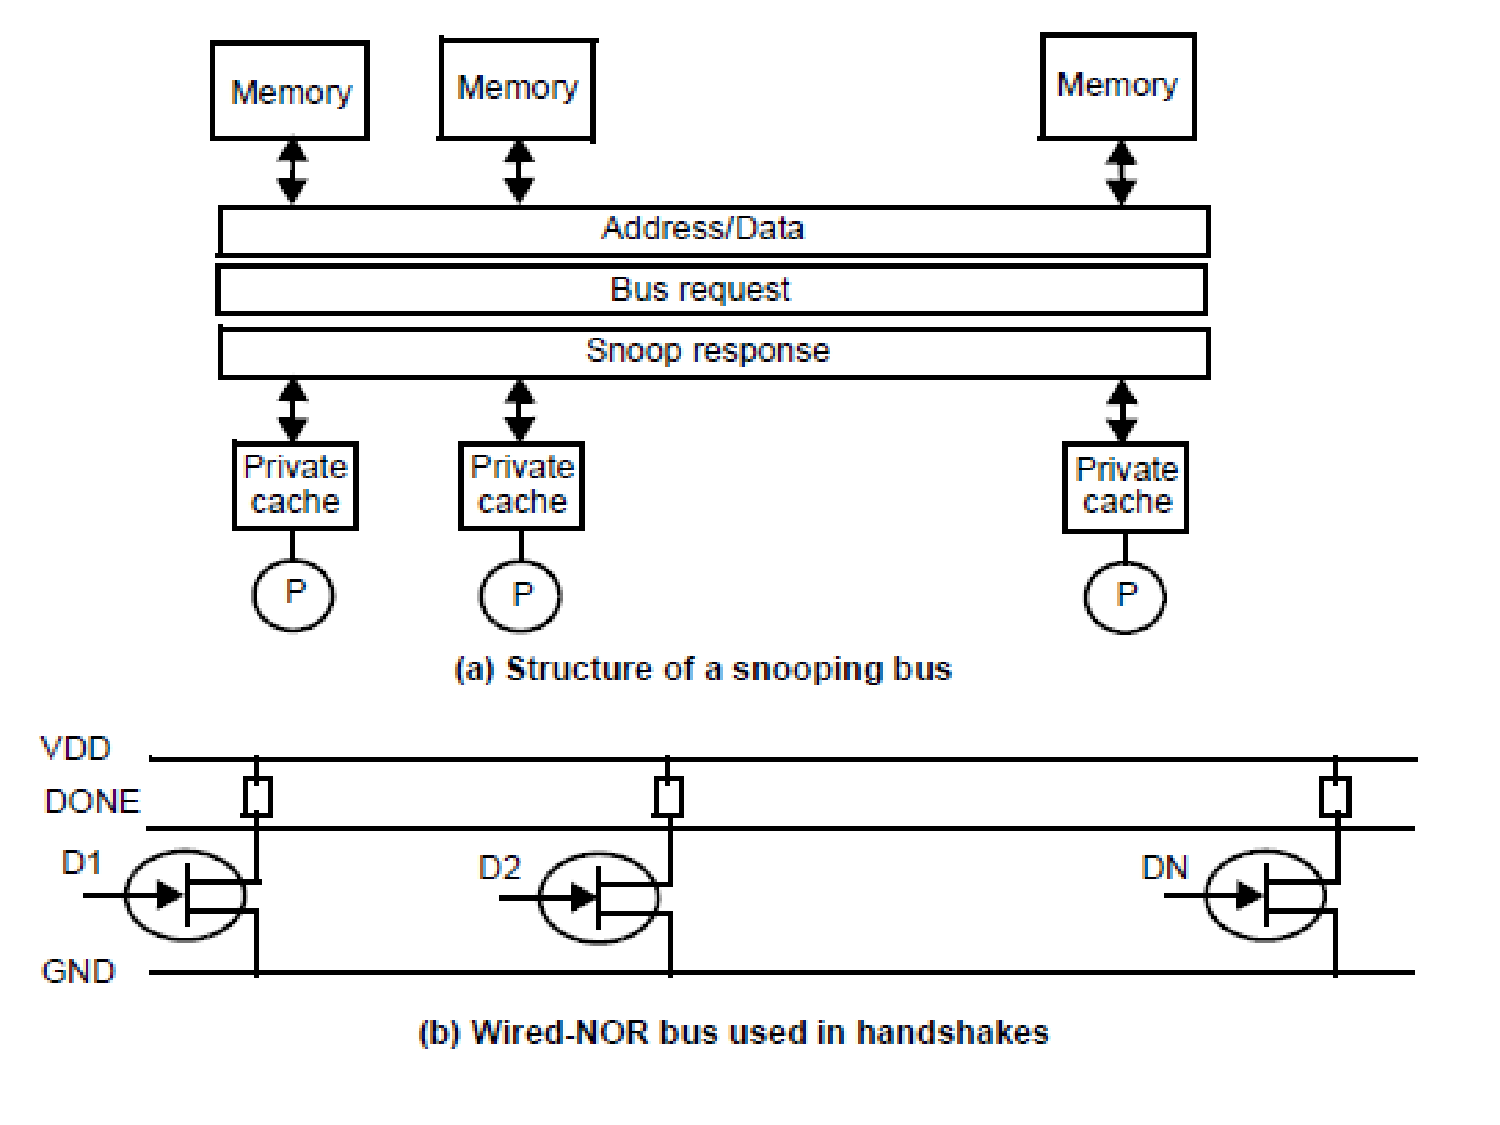
\includegraphics[width=47ex]{Figures/FigsInfCoherence/SnoopingBus}
\column{0.45\textwidth}
\vspace{-3ex}
\begin{scriptsize}
\begin{itemize}
    \item Transaction starts by supplying \emp{address/data} and a \emp{request}.
    \item and triggers a \emp{snoop action}, e.g., invalidate tag, and \emp{reply},
            e.g., when have all completed it?
    \item \emp{Synchronous} reply: establishes an upper-bound latency that 
            factors in conflicts $\Rightarrow$ use DualDirectory. 
    \item \emp{Asynchronous} by handshake (b):\\{{\tt NOR(D1,..,Dn)$\Rightarrow$ DONE}}, i.e.,\\
            {\tt If} any {\tt Di} is 1 {\tt Then} {\tt DONE} driven to ground 0
            {\tt Else} to supply volt 1. 
    \item \emp{Fetch from Remote or Memory?}\\
            $\overline{\mbox{\tt REMOTE}}${\tt=NOR(M1,..,Mn)}, where {\tt Mi} 
            is 1 when block in cache {\tt i} is in state M. Similar handshake.
\end{itemize}
\end{scriptsize}
\end{columns}

\begin{itemize}
    \item Initiate memory access in PARALLEL with snoop action, but memory responds 
        only after $\overline{\mbox{\tt REMOTE}}$ is known as 1.
    \item To reduce miss latency when it triggers replacement of M block $\Rightarrow$
            move block to \emp{victim buffer, which also supports snooping}.
\end{itemize} 

\end{frame}

\begin{frame}[fragile,t]
\frametitle{MESI Protocol for Write Back Caches}

MSI: read miss followed by write require TWO bus accesses.\smallskip

\emp{E(xclusive)} State entered on a read miss, when block is only in mem.\\
Uses a \emp{S(hared) bus line} to detect whether the copy will be unique.


\begin{columns}\hspace{-7ex}
\column{0.65\textwidth}
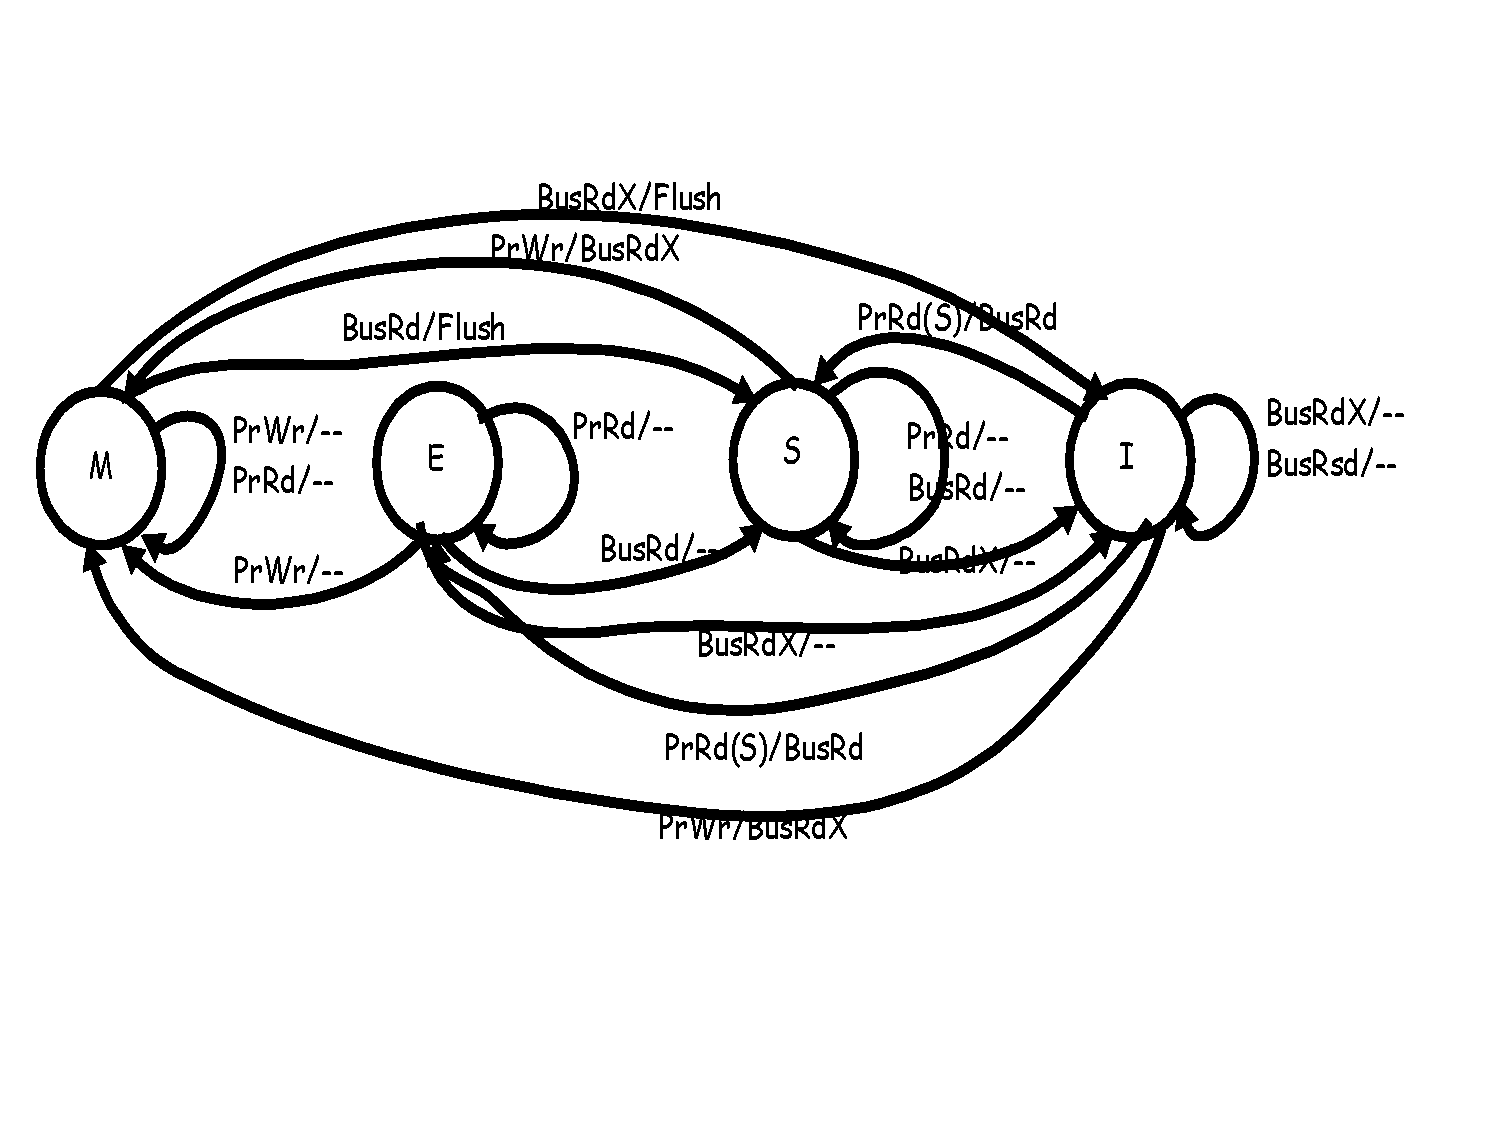
\includegraphics[width=55ex]{Figures/FigsInfCoherence/MESI}\pause
\column{0.38\textwidth}
\vspace{-3ex}
%\begin{scriptsize}
\begin{itemize}
    \item A read miss transitions from I to S if shared line is 1, and to E otherwise.
    \item If a block in E is updated ({\tt PrWr}) then E$\rightarrow$M without {\tt BusUpgr}.
    \item Could use {\tt BusUpgr} in transition S $\rightarrow$ M. 
\end{itemize}
%\end{scriptsize}
\end{columns}

\end{frame}

\begin{frame}[fragile,t]
\frametitle{MOESI: A General Class of Protocols}

MOESI adds a notion of ownership:
\begin{itemize}
    \item memory is eventually updated by owner (not at every write)
    \item allows cache-to-cache transfers between owner and requester
            (even when access was not exclusive).
\end  {itemize}


\begin{columns}\hspace{-5ex}
\column{0.65\textwidth}
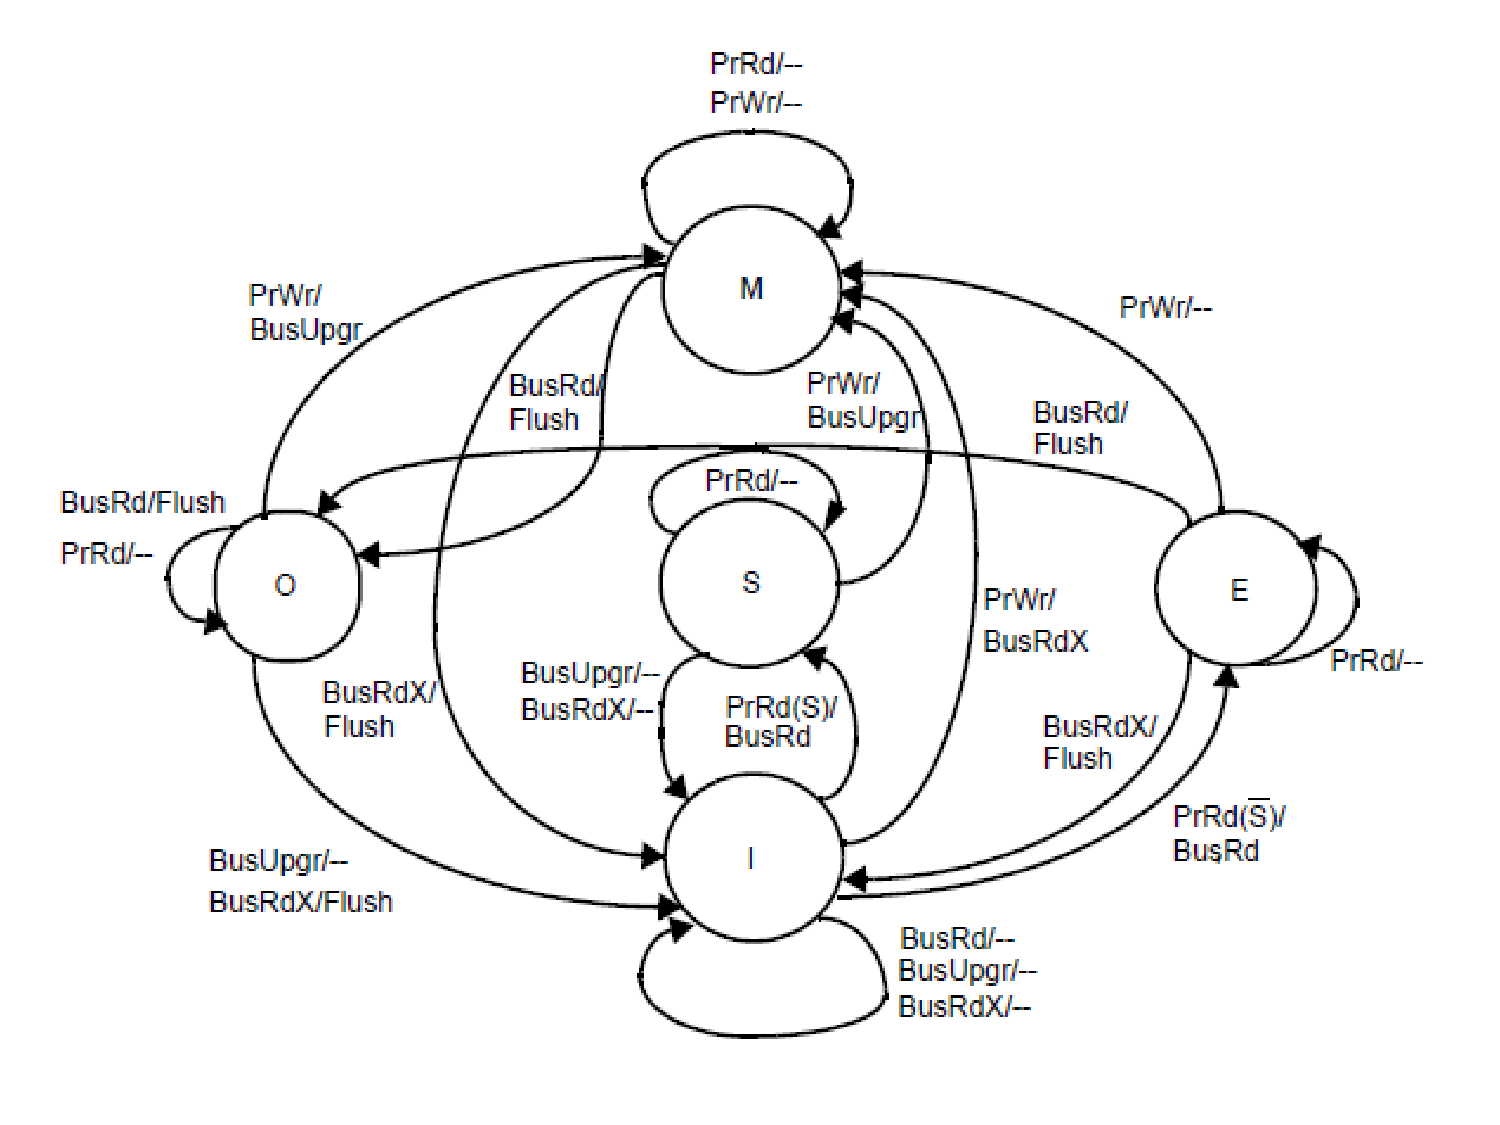
\includegraphics[width=45ex]{Figures/FigsInfCoherence/MOESI}
\column{0.38\textwidth}
%\begin{scriptsize}
\emp{Ownership transfered to another cache or memory when
block is invalidated or replaced!}
%\end{scriptsize}
\end{columns}

\end{frame}

\subsection{Cache Protocol Optimizations}
\begin{frame}[fragile,t]
\frametitle{Cache Protocol Optimizations}

\emph{Producer-Consumer Sharing via Read Snarfing (Broadcast):}
\begin{scriptsize}
\begin{itemize}
    \item {R$_i$/W$_i$} read/write of block A by processor {\tt i}. All caches have a copy of A.
    \item Sequence: {\tt W$_1$,R$_2$,R$_3$,..,R$_n$, W$_1$,R$_2$,R$_3$,..,R$_n$, ...}\pause
    \item \emp{results in an invalidation followed by $n-1$ read misses, all using the bus.}
    \item \emph{Optimized by letting the first read miss bring A into all caches.}
\end  {itemize}
\end{scriptsize}
\bigskip

\begin{block}{Migratory Sharing refers to data accessed in critical sections}
\begin{columns}
\column{0.22\textwidth}
\begin{colorcode}[fontsize=\scriptsize]
LOCK(LV);
    sum+=mysum;
UNLOCK(LV);
\end{colorcode} 
\column{0.75\textwidth}
\begin{scriptsize}
{\tt BusRd$_1$,BusUpgr$_1$, BusRd$_2$,BusUpgr$_2$, BusRd$_3$,BusUpgr$_3$, ...}\\
\emp{// $\downarrow$ Coherence miss then invalidation: combine Read \& Upgrade: $\downarrow$}\\
{\tt BusRdX$_1$, BusRdX$_2$, BusRdX$_2$, ...}
\end{scriptsize}
\end{columns}
\end{block}

Requires slight modificantions to MOESI, e.g., need to detect such sequences
and switch the optimization on/off.
\bigskip

\emph{Update-Based Protocols}: if every write is consumed by a different processor,
it is better to update eagerly all remote copies instead of invalidating them.
\emp{Optimizes latency and bandwidth.}

\end{frame}

\begin{frame}[fragile,t]
\frametitle{Write Back: MSI Update Protocol}

Dragon Multiprocessor (Xerox PARC 1980):\\
Same states as MOESI, but Invalid omitted to simplify.

\begin{columns}\hspace{-7ex}
\column{0.43\textwidth}
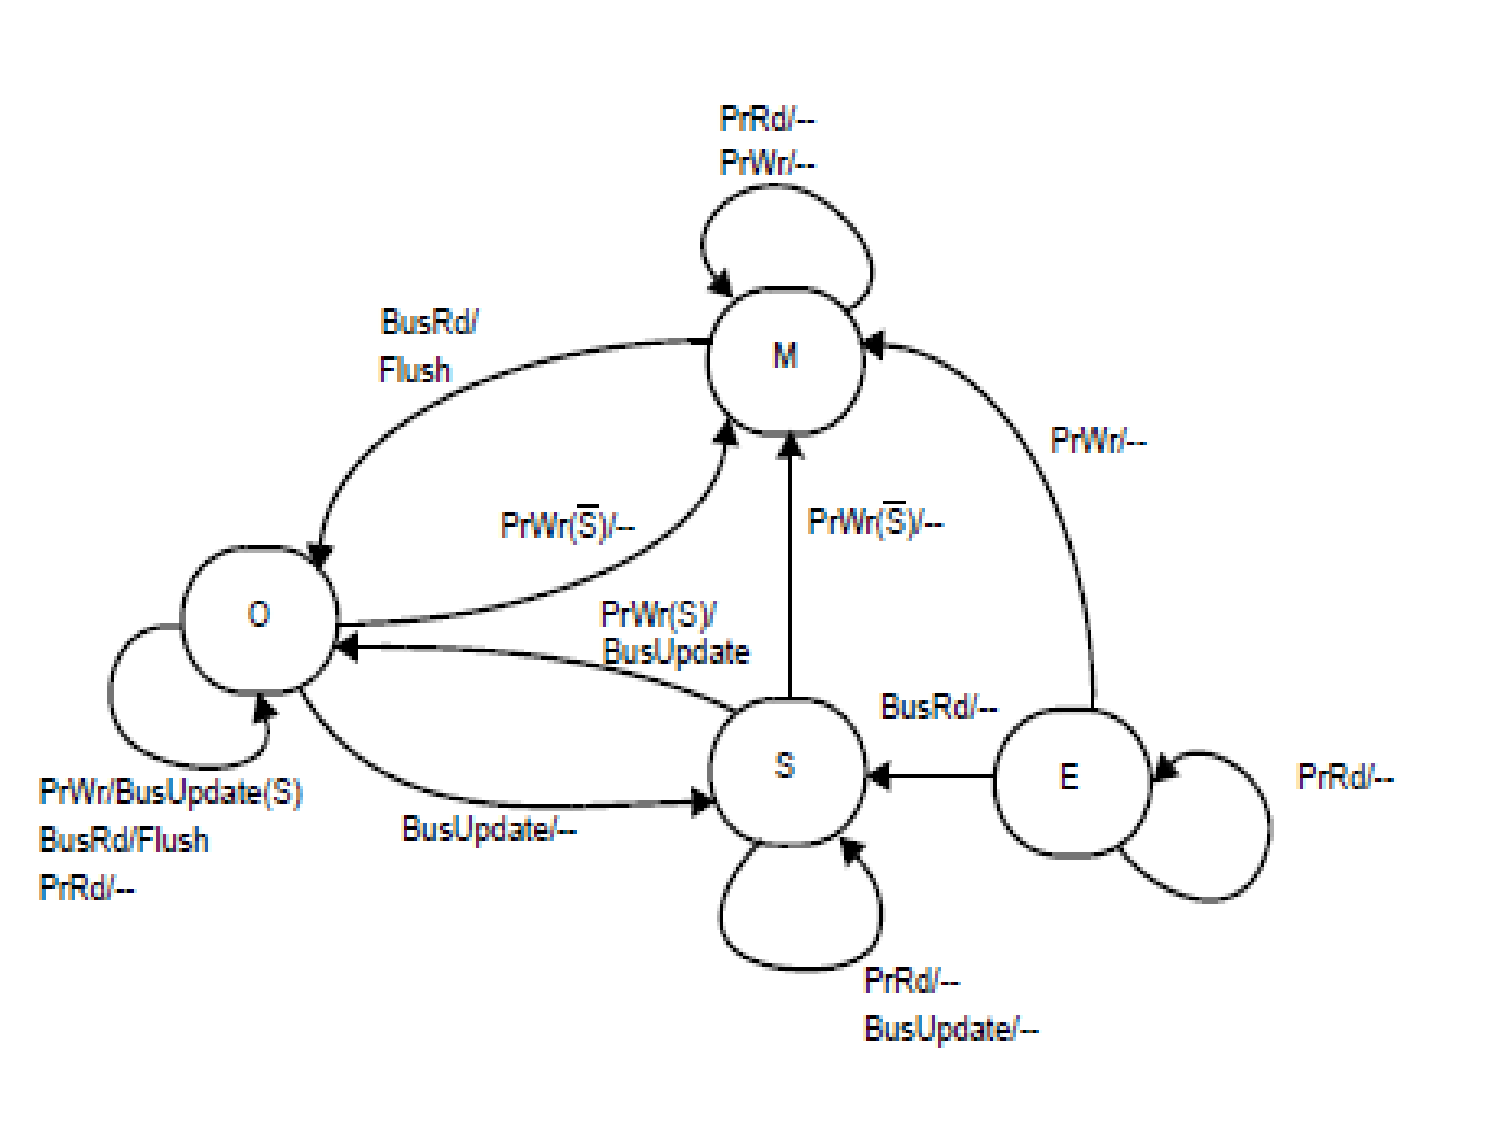
\includegraphics[width=40ex]{Figures/FigsInfCoherence/MSIupdate}\pause
\column{0.55\textwidth}
\begin{scriptsize}
\begin{itemize}
    \item[Shared] multiple copies, memory is clean. 
    \item[Modified] one copy, memory is stale, etc.
    \item[Transactions] BusRd requests a copy, BusUpdate updates remote copies.
    \item[S bus line] indicates whether remote copies exist.\bigskip
    \item[RdMiss] If no other cached copies, block loaded from mem in E,
                   Otherwise in S.\\
    \item[WrHit] If no other copies E$\rightarrow$M without using bus.\\
                 \emp{Else (Shared line 1) all copies are updated via 
                    {\tt BusUpdate}, and the update is propagated from owner.}  
\end{itemize}
\end{scriptsize}
\end{columns}
\bigskip
Under which program behavior is invalidation or update protocol best?

\end{frame}

\begin{frame}[fragile,t]
\frametitle{Comparison Invalidate vs Update Protocol}

\emp{Write-Run} of an access sequence to the same block is
the set of consecutive writes of the same processor before 
encountering a read/write of another processor.\\
\smallskip
Example: Write Run Length of {\tt R$_1$,W$_1$,R$_1$,W$_1$, W$_2$,R$_2$} is 2.
\bigskip

Bandwidth ({\tt B}) for a Write-Run of length N:
\begin{description}
    \item[INVALIDATE] {\tt B(UPGRADE) + B(READ MISS)}
    \item[UPDATE]     {\tt N $\times$ B(UPDATE)}
\end{description}

Assuming {\tt B(UPGRADE) $\equiv$ B(UPDATE)} then\\
\emp{Update outperforms Invalidate (i.e., uses less bandwidth) when}\\\pause
\emp{{\tt N < 1 + B(READ MISS)/B(UPDATE)}}
\medskip

This becomes: \emp{\tt N $<$ 1 + s}, where {\tt s} is the \# of words in a cache line, 
(because the update protocol updates only one word.)
\end{frame}

%%%%%%%%%%%%%%%%%%%%%%%%%%%%%%%%%%%%%%%%%%%
\subsection{Multiphase Cache Protocols}

\begin{frame}[fragile,t]
\frametitle{Multi-Phase Snoopy Cache Protocols}

\begin{columns}\hspace{-8ex}
\column{0.70\textwidth}
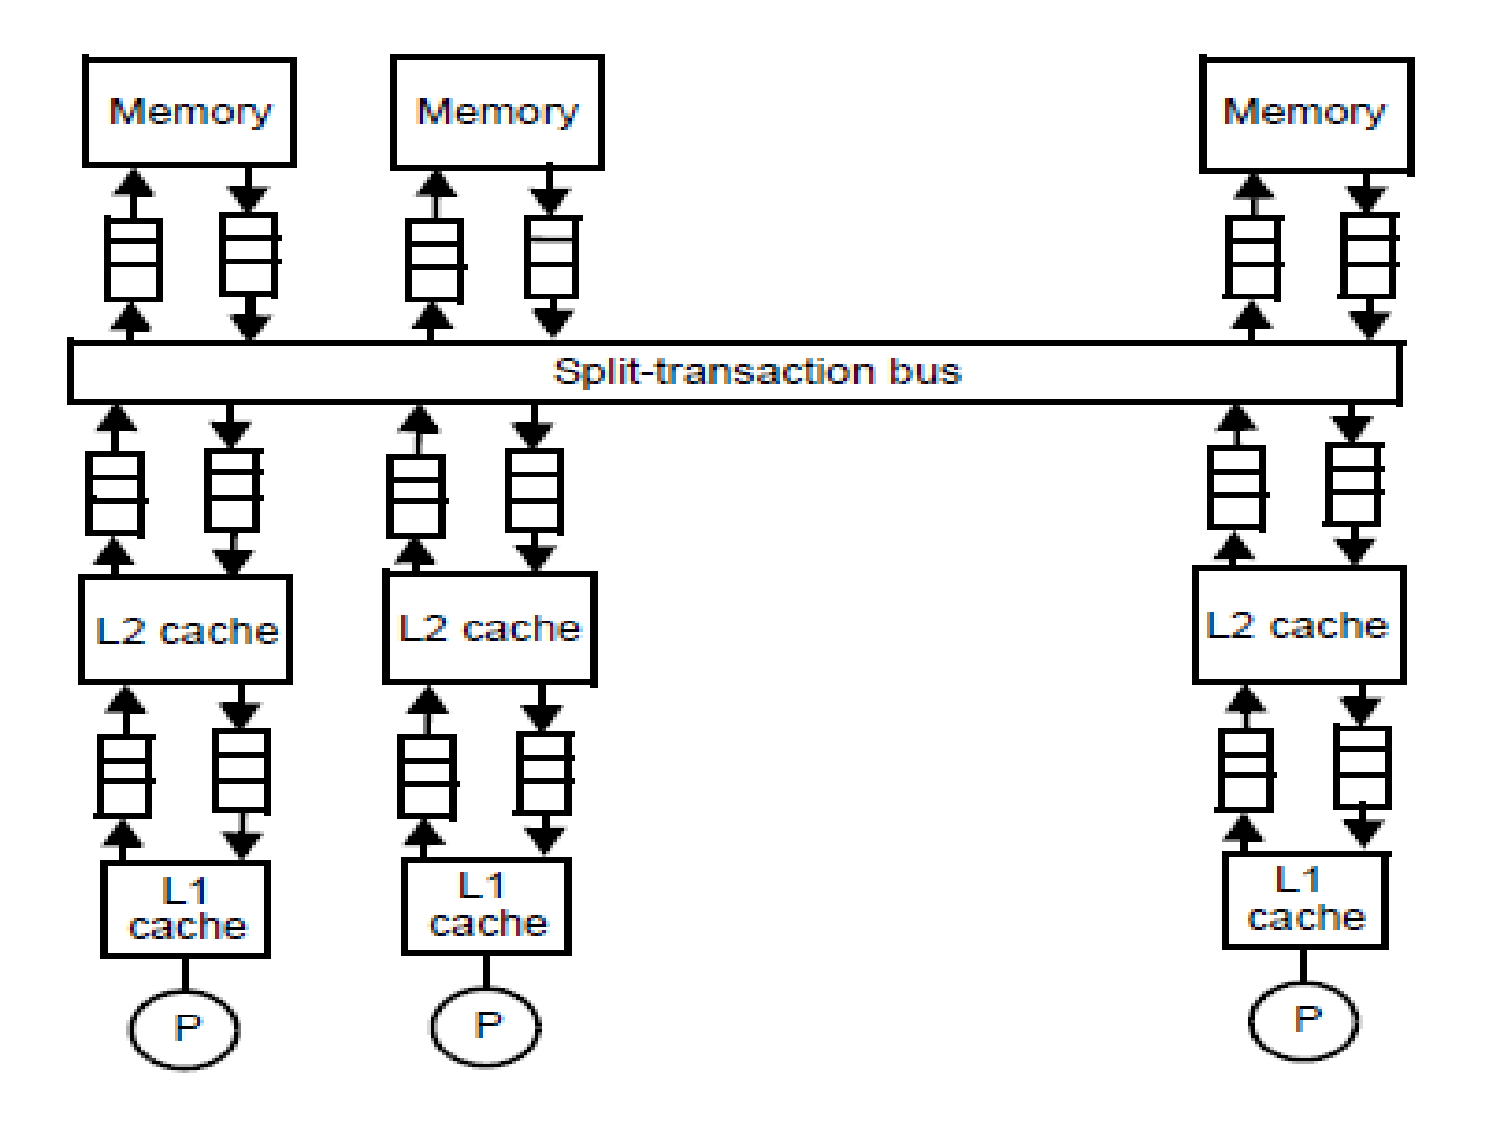
\includegraphics[width=50ex]{Figures/FigsInfCoherence/MultiLevCache}\pause
\column{0.28\textwidth}
\begin{scriptsize}
So far we have assumed:
\begin{itemize}
    \item single level of private cache, 
    \item and atomic pipelined buses.
\end{itemize}
\bigskip
\emp{A More Realistic Model:}
\begin{itemize}
    \item \emp{multi-level private cache hierarchy}
    \item \emp{a split transaction (pipelined) bus}\\
            {\em request \& response phases}
\end{itemize}
\end{scriptsize}
\end{columns}
\bigskip

Different caches/memory cannot consume requests at the same rate.
\emp{FIFO requests buffers} smooth out differences, and \emp{have a profound 
impact on the protocol design!}

\end{frame}

%\begin{frame}[fragile,t]
%\frametitle{REMEMBER Subtle Issue Slide?}
%
%\begin{columns}
%\column{0.48\textwidth}
%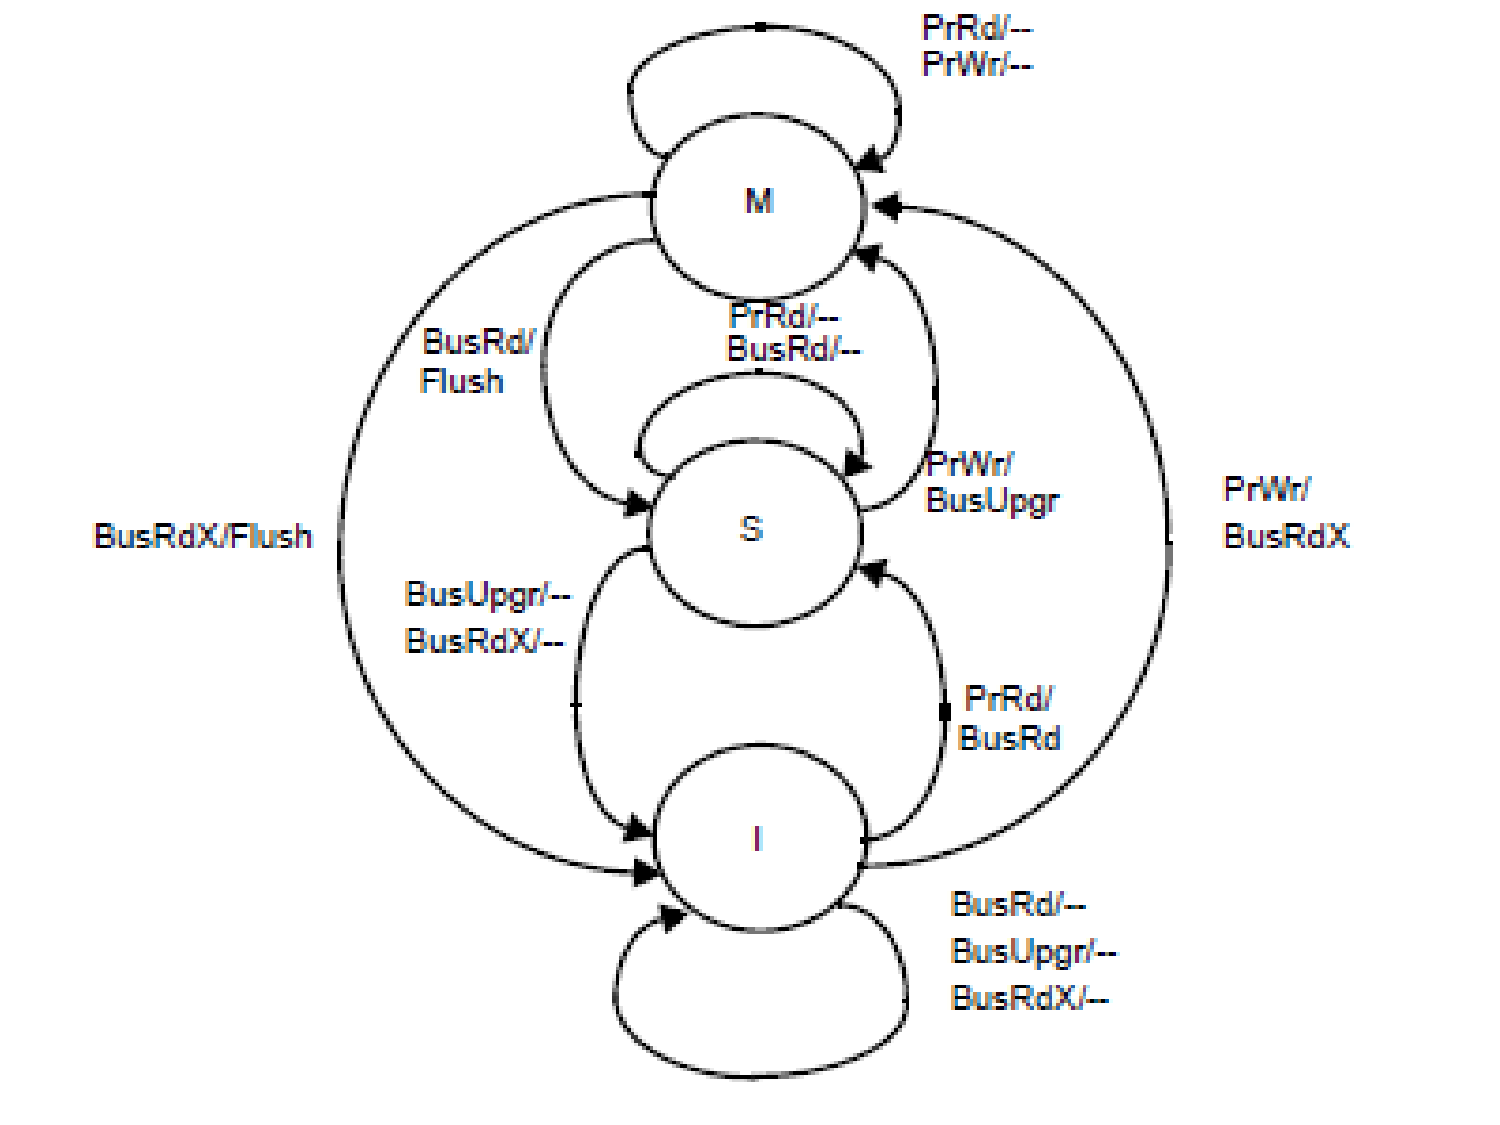
\includegraphics[width=35ex]{Figures/FigsInfCoherence/MSI}
%\column{0.48\textwidth}
%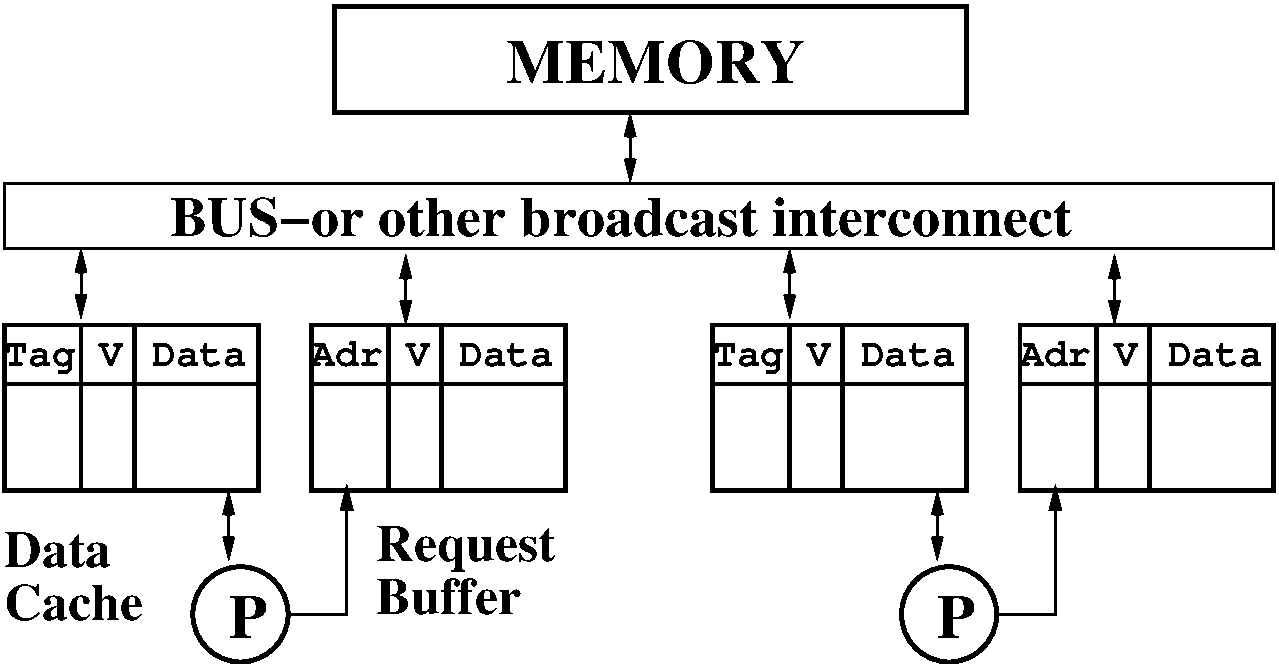
\includegraphics[width=30ex]{Figures/FigsInfCoherence/SMPreqbuff}
%\end{columns}
%
%\alert{Even the atomic protocols with a single level cache are too high level
%to resolve races in the presence of requests buffers.} Example MSI:%\begin{scriptsize}
%\begin{itemize}
%    \item P1 and P2 queue \emp{two {\tt BusUpgr}} to block A in request buffer. 
%    \item Assume P1 acquire bus while P2 waits in buffer. \alert{What happens?}
%    \item P1's {\tt BusUpgr} should move P2 to Invalid state, hence
%    \item when P2 acquires bus, should send a \emp{\tt BusRdX} (not {\tt BusWrite}).
%\end{itemize}
%
%\end{frame}

\begin{frame}[fragile,t]
\frametitle{Atomic Transaction Disadvantages}
Example: bus clocked at 100MHz can transfer 3 parallel segments in one cycle: 
(1) a request, (2) an address and (3) 256-bits of data. Assume no caches and
that memory is banked and can supply a 32-byte cache block in 200 ns. 
\alert{What fraction of the time will the atomic bus be idle?}
\bigskip\pause

1 clock cycle: {\tt 1sec / freq = 10ns}.\\ 
Bus is idle: $200/220 = 91$\% of time.

\end{frame}


\begin{frame}[fragile,t]
\frametitle{Transient Non-Atomic Cache States for MSI}

\alert{Even the atomic protocols with a single level cache are too high level
to resolve races in the presence of requests buffers.}\medskip

Transient states SM, IM are needed to cope with 
non-atomic (multi-phase) transactions. \smallskip

\begin{columns}\hspace{-5ex}
\column{0.55\textwidth}
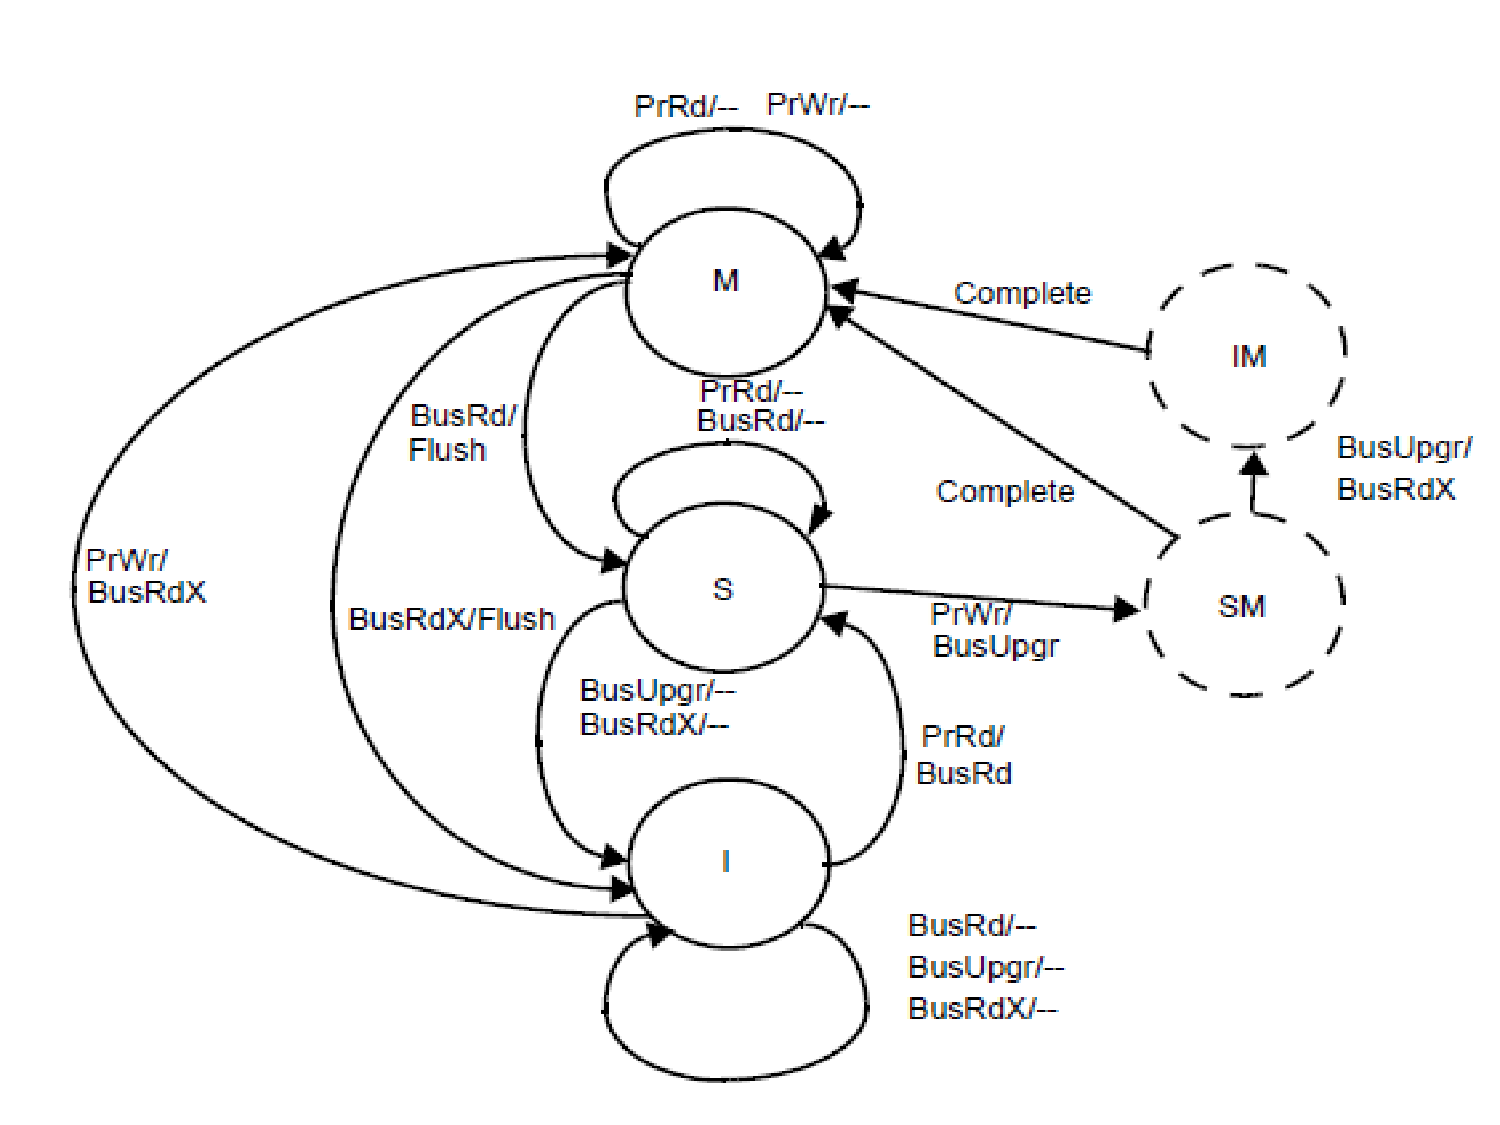
\includegraphics[width=44ex]{Figures/FigsInfCoherence/MSInonatomicStates}\pause
\column{0.43\textwidth}
\begin{scriptsize}
\begin{itemize}
    \item On a P1 write hit a block in S transitions to SM and enqueues {\tt BusUpgr}.
    \item If a {\tt BusUpgr} received from P2 before P1 transact completed,\\ 
          Then P1 goes to IM and {\tt BusRdX} replaces {\tt BusUpgr} in buffer. 
    \item Eventually, when transition completed, i.e., request sent and reply received,
            P1 goes to M.
\end{itemize}
\end{scriptsize}
\end{columns}
\bigskip

\end{frame}

\begin{frame}[fragile,t]
\frametitle{Split-Transaction Bus}

Pipelines a sequence of phases in a bus transaction,
e.g., arbitration, transfer, response.\bigskip

Dividing a transaction into subtransactions $\Rightarrow$
Tradeoff between \pause additional latency (repeated bus arbitration) and better bandwidth.\bigskip

Pipeline stages must be balanced to maximize throughput.\bigskip

For example, if both request and response transfer use the address bus,
they can only be pipelined:
\vspace{-4ex}

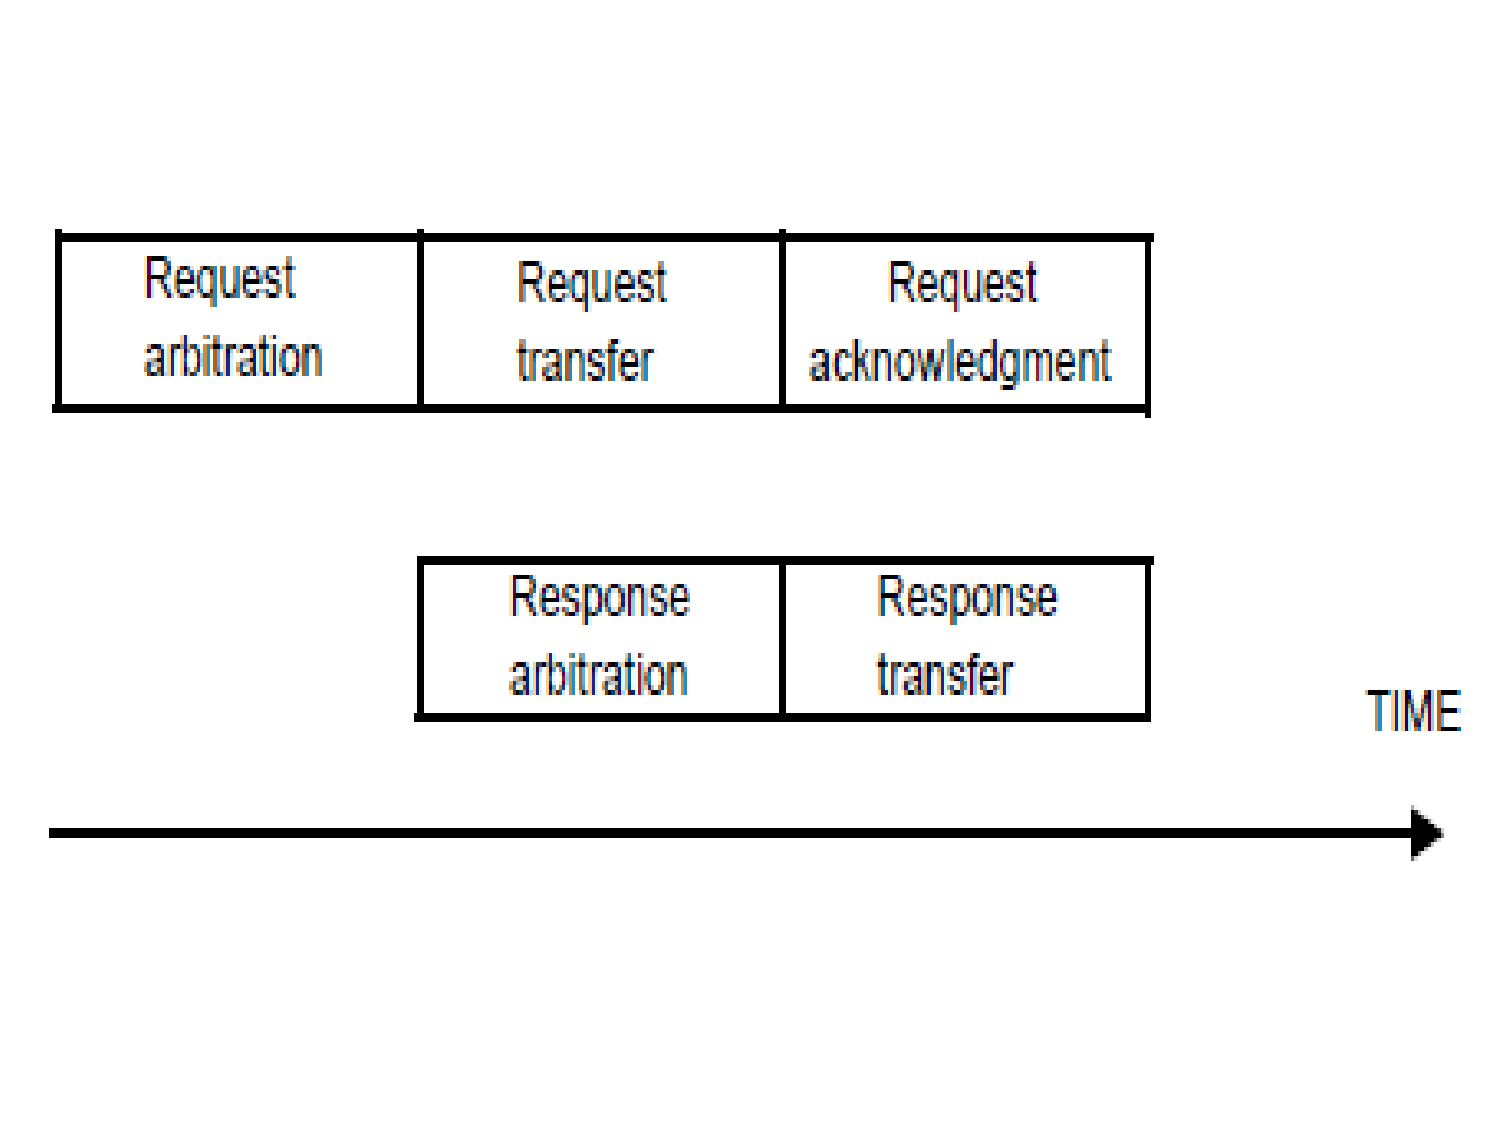
\includegraphics[width=44ex]{Figures/FigsInfCoherence/SplitTransBus}

\end{frame}

\begin{frame}[fragile,t]
\frametitle{Access Races on Split-Transaction Buses}

Are dealt via transient states, a ``simple'' implementation is: %but additional issues are:
\begin{itemize}
    \item[1] \emp{Resolve conflicting requests (to the same address):}\\
            \begin{itemize} 
                \item use request tables monitored by all nodes;
                \item request launched only if no entry in the table matches its address 
                \item $\Rightarrow$ only one request to same address in the system at a time.
            \end{itemize} 
    \item[2] \emp{How to report snoop results, e.g., shared line?}
            \begin{itemize} 
                \item snoop result needed to transition in new state, 
                        hence it should be part of request phase,
                \item but inbound buffers, e.g., bus to cache) would add too big a delay. 
                \item $\Rightarrow$ Essential to look directly in CacheDir before buffering.
                \item Requires \emph{1} to work correctly.
            \end{itemize} 
    \item[3] \emp{Prevent buffer overflows:}
            \begin{itemize} 
                \item Add provisions in protocol to {\tt NACK} when buffers overflow, i.e.,
                \item Do not start transaction until all relevant FIFO buffers have space. 
            \end{itemize}             
\end{itemize}

This is part of the solution of SGI Challenge mid90s.

\end{frame}


\begin{frame}[fragile,t]
\frametitle{Multi-Level Cache Issues}

Adding another level of private cache offers benefits:
\begin{itemize} 
    \item shorter miss penalty to next level,
    \item filters out snoop actions to first level $\Rightarrow$
    \item \emph{less proc-bus conflicts on L1 cache \& less snoop latency!}
    \item especially if cache inclusion is maintained
            (e.g., it can be forced by evicting an L1 
            block when is evicted from L2.)
\end{itemize} 
\bigskip

Write Policy is important to reduce snoop overhead:
\begin{itemize}
    \item If L1 is write-back Then L2's copy is inconsistent and
            dirty miss requests must be serviced by L1.\pause
    \item \emph{If L1 is write-through and inclusion is maintained $\Rightarrow$
                L2 is consistent and can service all miss requests from
                other processors,}
    \item which can significantly improve performance.
\end{itemize}

\end{frame}

%%%%%%%%%%%%%%%%%%%%%%%%%%%%%%%%%%%%%%%%%%%
\subsection{Cache Miss Classification (Updated)}
\begin{frame}[fragile,t]
\frametitle{True vs False Sharing}

\emph{True Sharing Communicates Values (Essential):}
\begin{itemize} 
    \item Two processors access the same word. \emp{Remember:}
    \item Update protocol better for Fine-Grained Sharing (short Write Runs)
    \item Invalidate better for Coarse-Grain Sharing: {\tt N $>$ 1+b},\\
            where {\tt b} is \# of words in a cache line,
                    {\tt N} is the write-run length.
\end{itemize} 
\bigskip

\alert{False Sharing Does Not Communicate Values (pure overhead)}
\begin{itemize}
    \item P1 and P2 access two different words in the same block.
    \item Write Invalidate causes false sharing misses, e.g., P1 write {\tt W1} then
            P2 reads {\tt W2}, where {\tt W1} and {\tt W2} are distinct words in the same block. 
    \item Write Update causes false sharing updates to dead copies.
\end{itemize}

\end{frame}

\begin{frame}[fragile,t]
\frametitle{Essential vs Non-Essential Misses}

Assume A, B, C belong to same block B1, and D to another block
\begin{tabular}{lllll}
\hline
Time    & Proc1 & Proc2 & Proc3 & Miss Type \\\hline
1       & R$_A$ &       &       & Cold      \\
2       &       & R$_B$ &       & Cold      \\
3       &       &       & R$_C$ & Cold      \\
4       &       &       & R$_D$(evict B1) & Cold      \\
5       & W$_A$ &       &       &           \\
6       &       & R$_A$ &       & True Sharing      \\
7       & W$_B$ &       &       &           \\
8       &       & R$_A$ &       & False Sharing     \\
9       &       &       & R$_C$ & Replacement \\\hline
\end{tabular}
\bigskip

Cold, True Sharing (coherence), and replacement (conflict or capacity)
misses are \emph{Essential}; False Sharing misses are \alert{Non Essential}.\bigskip

Same reasoning can be applied to memory traffic.
\end{frame}

\begin{frame}[fragile,t]
\frametitle{Classification of Misses}
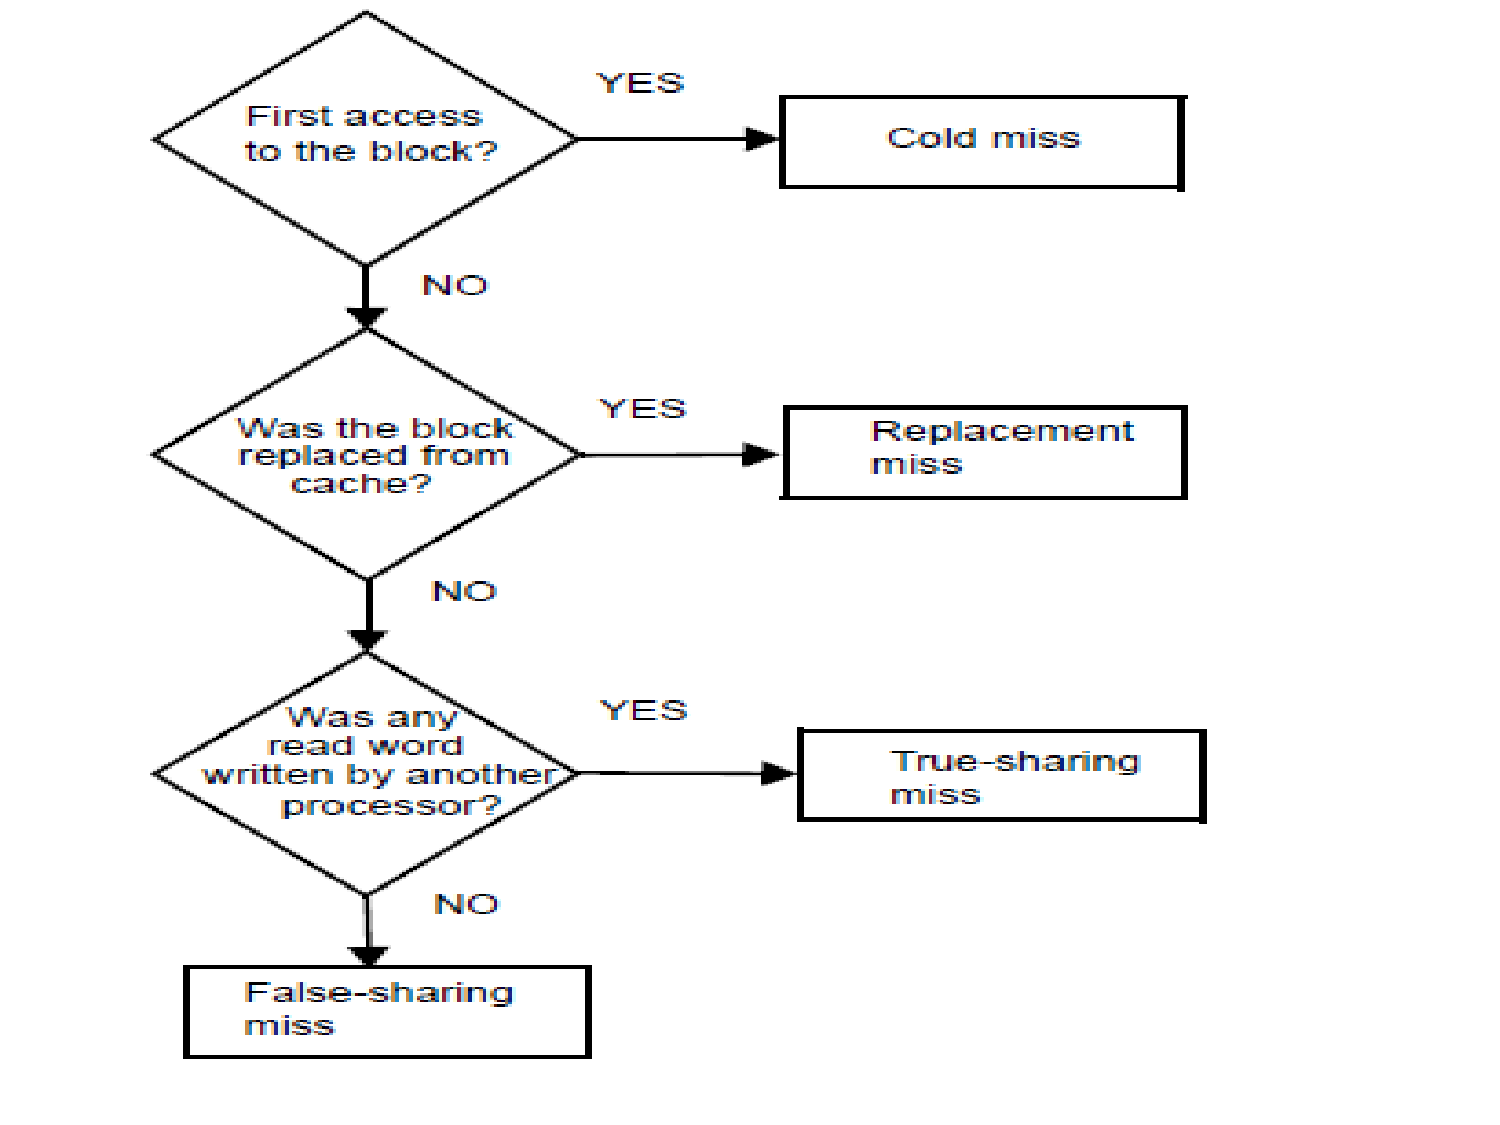
\includegraphics[width=59ex]{Figures/FigsInfCoherence/MissClassif}
\end{frame}

%%%%%%%%%%%%%%%%%%%%%%%%%%%%%%%%%%%%%%%%%%%
\subsection{Translation Lookahead Buffer (TLB) Consistency}
\begin{frame}[fragile,t]
\frametitle{Recall Translation Lookahead Buffer}
\bigskip

\emph{Virtual Memory (VM) manages the Main Memory (MM) ``cache'' by 
migrating fixed-size memory pages between MM and Disk:}
\begin{itemize} 
    \item Page Tables are stored in MM and keep track of the pages resident in MM 
    \item A VM Address is translated to a Physical-MM Address,
            with the use of \emp{hardware support}:
    \item TLB is a cache for virtual-to-physical translations and typically sits 
            between processor and L1 cache. \alert{Why?}
%            (because processor addresses are virtual,
%            but we have assumed caches are addressable via physical-MM address).
\end{itemize} 
\bigskip

In a multiprocessor, TLBs act as private caches and\\
\alert{Consistency Between TLBs is Essential For Correct Execution}
\end{frame}

\begin{frame}[fragile,t]
\frametitle{Sources of TLB Inconsistency}
\bigskip

TLB is inconsistent when one of its entries differs from the Page-Table Entry.
\emp{Sources of Inconsistency:}
\begin{itemize} 
    \item A page is evicted and replaced with another: An unaware TLB
            maps now addresses of the evicted page to the new
            loaded page \& also all the cached blocks of the old page are stale.
    \item Access rights are changed: An unaware TLB would not enforce the
            more restrictive rights or generates unnecessary exceptions.
    \item Access statistics are changed (page becomes dirty): may loose the
            updates of the inconsistent TLB. 
\end{itemize} 
\bigskip

Not all critical for correctness, e.g., reference-bit inconsistency 
leads to suboptimal VM manager decisions.

\end{frame}

\begin{frame}[fragile,t]
\frametitle{Enforcing TLB Consistency}
\bigskip

One Solution is \emp{TLB SHOOTDOWN}:
\begin{itemize} 
    \item[1] On page eviction the Master processor (executing the VM manager)
                locks the page table entry, and
    \item[2] Sends interrupt signals to all processors involved. 
    \item[3] Each processor invalidates the inconsistent TLB entry
    \item[4] Each processor invalidates the inconsistent cache entries
    \item[5] Each processor acknowledges back to Master.
    \item[6] Master replaces the page and unlocks the page-table entry.
\end{itemize} 

\bigskip
\alert{TLB shootdown is expensive}, \emph{but luckily it happens rarely!}

\end{frame}


\end{document}
